% Options for packages loaded elsewhere
\PassOptionsToPackage{unicode}{hyperref}
\PassOptionsToPackage{hyphens}{url}
\PassOptionsToPackage{dvipsnames,svgnames,x11names}{xcolor}
%
\documentclass[
  letterpaper,
  DIV=11,
  numbers=noendperiod]{scrreprt}

\usepackage{amsmath,amssymb}
\usepackage{iftex}
\ifPDFTeX
  \usepackage[T1]{fontenc}
  \usepackage[utf8]{inputenc}
  \usepackage{textcomp} % provide euro and other symbols
\else % if luatex or xetex
  \usepackage{unicode-math}
  \defaultfontfeatures{Scale=MatchLowercase}
  \defaultfontfeatures[\rmfamily]{Ligatures=TeX,Scale=1}
\fi
\usepackage{lmodern}
\ifPDFTeX\else  
    % xetex/luatex font selection
\fi
% Use upquote if available, for straight quotes in verbatim environments
\IfFileExists{upquote.sty}{\usepackage{upquote}}{}
\IfFileExists{microtype.sty}{% use microtype if available
  \usepackage[]{microtype}
  \UseMicrotypeSet[protrusion]{basicmath} % disable protrusion for tt fonts
}{}
\makeatletter
\@ifundefined{KOMAClassName}{% if non-KOMA class
  \IfFileExists{parskip.sty}{%
    \usepackage{parskip}
  }{% else
    \setlength{\parindent}{0pt}
    \setlength{\parskip}{6pt plus 2pt minus 1pt}}
}{% if KOMA class
  \KOMAoptions{parskip=half}}
\makeatother
\usepackage{xcolor}
\setlength{\emergencystretch}{3em} % prevent overfull lines
\setcounter{secnumdepth}{4}
% Make \paragraph and \subparagraph free-standing
\makeatletter
\ifx\paragraph\undefined\else
  \let\oldparagraph\paragraph
  \renewcommand{\paragraph}{
    \@ifstar
      \xxxParagraphStar
      \xxxParagraphNoStar
  }
  \newcommand{\xxxParagraphStar}[1]{\oldparagraph*{#1}\mbox{}}
  \newcommand{\xxxParagraphNoStar}[1]{\oldparagraph{#1}\mbox{}}
\fi
\ifx\subparagraph\undefined\else
  \let\oldsubparagraph\subparagraph
  \renewcommand{\subparagraph}{
    \@ifstar
      \xxxSubParagraphStar
      \xxxSubParagraphNoStar
  }
  \newcommand{\xxxSubParagraphStar}[1]{\oldsubparagraph*{#1}\mbox{}}
  \newcommand{\xxxSubParagraphNoStar}[1]{\oldsubparagraph{#1}\mbox{}}
\fi
\makeatother


\providecommand{\tightlist}{%
  \setlength{\itemsep}{0pt}\setlength{\parskip}{0pt}}\usepackage{longtable,booktabs,array}
\usepackage{calc} % for calculating minipage widths
% Correct order of tables after \paragraph or \subparagraph
\usepackage{etoolbox}
\makeatletter
\patchcmd\longtable{\par}{\if@noskipsec\mbox{}\fi\par}{}{}
\makeatother
% Allow footnotes in longtable head/foot
\IfFileExists{footnotehyper.sty}{\usepackage{footnotehyper}}{\usepackage{footnote}}
\makesavenoteenv{longtable}
\usepackage{graphicx}
\makeatletter
\newsavebox\pandoc@box
\newcommand*\pandocbounded[1]{% scales image to fit in text height/width
  \sbox\pandoc@box{#1}%
  \Gscale@div\@tempa{\textheight}{\dimexpr\ht\pandoc@box+\dp\pandoc@box\relax}%
  \Gscale@div\@tempb{\linewidth}{\wd\pandoc@box}%
  \ifdim\@tempb\p@<\@tempa\p@\let\@tempa\@tempb\fi% select the smaller of both
  \ifdim\@tempa\p@<\p@\scalebox{\@tempa}{\usebox\pandoc@box}%
  \else\usebox{\pandoc@box}%
  \fi%
}
% Set default figure placement to htbp
\def\fps@figure{htbp}
\makeatother
% definitions for citeproc citations
\NewDocumentCommand\citeproctext{}{}
\NewDocumentCommand\citeproc{mm}{%
  \begingroup\def\citeproctext{#2}\cite{#1}\endgroup}
\makeatletter
 % allow citations to break across lines
 \let\@cite@ofmt\@firstofone
 % avoid brackets around text for \cite:
 \def\@biblabel#1{}
 \def\@cite#1#2{{#1\if@tempswa , #2\fi}}
\makeatother
\newlength{\cslhangindent}
\setlength{\cslhangindent}{1.5em}
\newlength{\csllabelwidth}
\setlength{\csllabelwidth}{3em}
\newenvironment{CSLReferences}[2] % #1 hanging-indent, #2 entry-spacing
 {\begin{list}{}{%
  \setlength{\itemindent}{0pt}
  \setlength{\leftmargin}{0pt}
  \setlength{\parsep}{0pt}
  % turn on hanging indent if param 1 is 1
  \ifodd #1
   \setlength{\leftmargin}{\cslhangindent}
   \setlength{\itemindent}{-1\cslhangindent}
  \fi
  % set entry spacing
  \setlength{\itemsep}{#2\baselineskip}}}
 {\end{list}}
\usepackage{calc}
\newcommand{\CSLBlock}[1]{\hfill\break\parbox[t]{\linewidth}{\strut\ignorespaces#1\strut}}
\newcommand{\CSLLeftMargin}[1]{\parbox[t]{\csllabelwidth}{\strut#1\strut}}
\newcommand{\CSLRightInline}[1]{\parbox[t]{\linewidth - \csllabelwidth}{\strut#1\strut}}
\newcommand{\CSLIndent}[1]{\hspace{\cslhangindent}#1}

\KOMAoption{captions}{tableheading}
\makeatletter
\@ifpackageloaded{bookmark}{}{\usepackage{bookmark}}
\makeatother
\makeatletter
\@ifpackageloaded{caption}{}{\usepackage{caption}}
\AtBeginDocument{%
\ifdefined\contentsname
  \renewcommand*\contentsname{Tabla de contenidos}
\else
  \newcommand\contentsname{Tabla de contenidos}
\fi
\ifdefined\listfigurename
  \renewcommand*\listfigurename{Listado de Figuras}
\else
  \newcommand\listfigurename{Listado de Figuras}
\fi
\ifdefined\listtablename
  \renewcommand*\listtablename{Listado de Tablas}
\else
  \newcommand\listtablename{Listado de Tablas}
\fi
\ifdefined\figurename
  \renewcommand*\figurename{Figura}
\else
  \newcommand\figurename{Figura}
\fi
\ifdefined\tablename
  \renewcommand*\tablename{Tabla}
\else
  \newcommand\tablename{Tabla}
\fi
}
\@ifpackageloaded{float}{}{\usepackage{float}}
\floatstyle{ruled}
\@ifundefined{c@chapter}{\newfloat{codelisting}{h}{lop}}{\newfloat{codelisting}{h}{lop}[chapter]}
\floatname{codelisting}{Listado}
\newcommand*\listoflistings{\listof{codelisting}{Listado de Listados}}
\makeatother
\makeatletter
\makeatother
\makeatletter
\@ifpackageloaded{caption}{}{\usepackage{caption}}
\@ifpackageloaded{subcaption}{}{\usepackage{subcaption}}
\makeatother

\ifLuaTeX
\usepackage[bidi=basic]{babel}
\else
\usepackage[bidi=default]{babel}
\fi
\babelprovide[main,import]{spanish}
% get rid of language-specific shorthands (see #6817):
\let\LanguageShortHands\languageshorthands
\def\languageshorthands#1{}
\usepackage{bookmark}

\IfFileExists{xurl.sty}{\usepackage{xurl}}{} % add URL line breaks if available
\urlstyle{same} % disable monospaced font for URLs
\hypersetup{
  pdftitle={Informe ID21I10297},
  pdfauthor={M. Abel Herrera y Francisco Zambrano},
  pdflang={es},
  colorlinks=true,
  linkcolor={blue},
  filecolor={Maroon},
  citecolor={Blue},
  urlcolor={Blue},
  pdfcreator={LaTeX via pandoc}}


\title{Informe ID21I10297}
\author{M. Abel Herrera y Francisco Zambrano}
\date{2025-03-21}

\begin{document}
\maketitle

\renewcommand*\contentsname{Tabla de contenidos}
{
\hypersetup{linkcolor=}
\setcounter{tocdepth}{2}
\tableofcontents
}

\part{Acerca del Informe}

Reporte general del proyecto ID21I10297, financiado por la Agencia
Nacional de Investigación y Desarrollo (ANID) por medio del proyecto
FONDEF IDEA 2021.

Esto proyecto estuvo a cargo del director Dr.~Francisco Zambrano
Bigiarini de la Universidad Mayor.

Investigadores que participaron el el proyecto:

\begin{itemize}
\tightlist
\item
  Dr.~Francisco Zambrano - Director - Centro Hemera UMayor
\item
  Dra. Andrea Miyasaka Almeyda - Directora Alterna - Centro CGB UMayor
\item
  Dr.~Felipe de La Hoz - Investigador - Externo
\item
  Paulina Vidal - Investigadora - Centro Hemera UMayor
\item
  Idania Briceño - Investigadora - Centro Hemera UMayor
\end{itemize}

Además, trabajaron como asistentes de investigación los siguientes
profesionales:

\begin{itemize}
\tightlist
\item
  Jesica Garrido - Centro Hemera UMayor
\item
  Abel Herrera - Centro Hemera UMayor
\end{itemize}

\bookmarksetup{startatroot}

\chapter*{Prefacio}\label{prefacio}
\addcontentsline{toc}{chapter}{Prefacio}

\markboth{Prefacio}{Prefacio}

Este informe presenta metodología y los resultados obtenidos en el marco
del proyecto FONDEF ID21I10297. En este proyecto se desarrolló
\href{https://s4tori.cl}{SatOri}, una aplicación para la optimización de
riego en frutales. La que contribuye a la adaptación al cambio climático
de la agricultura chilena.

\texttt{SatOri} desarrolló un modelo para la estimación espacial con
frecuencia diaria del potencial hídrico xilemático (\(\Psi_x\)). El
\(Psi_x\) permite monitorear la respuesta de la planta a las condiciones
medio ambientales y de abastecimiento hídrico. Se utilizaron algoritmos
de machine learning, datos meteorológicos y de imagenes satelitales
Sentine-2, para el desarrollo del modelo.

Por otra parte, \texttt{SatOri} calcula el nivel de \(Psi_x\) mínimo que
pueden alcanzar los árboles. De esta manerá establece un semáforo de
acuerdo a este umbral y a los resultados del modelo. Indicando al
agricultor cuanto es el tiempo de riego que debe suministrar acada
sector, para que no se vea afectado el aparato fotosintético de la
planta y así no haya merma en la producción y calidad de la fruta.

\part{Introducción}

\chapter{Resumen}\label{resumen}

{[}Resumen{]}

\chapter{Introducción}\label{introducciuxf3n-1}

El cambio climático ha intensificado la sequía en diversas regiones del
mundo, afectando particularmente a Chile Central, donde se ha registrado
un evento de Mega Sequía sin precedentes en los últimos milenios. Desde
2010, la zona ha experimentado una reducción sostenida de las
precipitaciones, con déficits promedio entre 20-40\% (Garreaud et
al.~2020). Este fenómeno impacta directamente la disponibilidad hídrica
para la agricultura, con repercusiones en la productividad y
sostenibilidad del sector (Peña-Guerrero et al.~2020). Ante este
escenario, se requieren estrategias de gestión del agua más eficientes
que permitan a los productores agrícolas adaptarse a la variabilidad
climática (Hurlbert y Gupta 2017).

En este contexto, el riego deficitario controlado (RDC) ha sido
identificado como una estrategia eficaz para optimizar el uso del agua
en cultivos perennes como los frutales, donde las opciones de adaptación
son limitadas (Pechan et al.~2023). Esta práctica permite reducir el
consumo hídrico sin afectar significativamente la producción ni la
calidad de la cosecha, mejorando la eficiencia del recurso disponible
(Victor Blanco et al.~2019; López-Olivari y Ortega-Klose 2021). Entre
los frutales de exportación, el cerezo es el segundo producto de mayor
valor en la agroindustria chilena, con más de 25 000 hectáreas bajo
riego y un mercado aproximado de 1560 millones de dólares
(Carrasco-Benavides, Antunez-Quilobrán, et al.~2020; González 2022). La
optimización del riego en este cultivo es fundamental para mejorar la
sostenibilidad del sector y mantener su competitividad a nivel
internacional.

La presente investigación tiene como objetivo desarrollar un prototipo
de servicio web para la optimización del riego en cerezo (SatOri), que
permita a los productores ajustar los tiempos y volúmenes de riego en
función de datos obtenidos de sensores satelitales ópticos y de radar,
complementados con ensayos de riego deficitario controlado. Para ello,
se evaluará el nivel de riego deficitario óptimo en huertos de cerezo
ubicados en la región de O'Higgins durante las temporadas 2022-2023,
desarrollando un modelo de estimación del potencial hídrico xilemático
(Ψs) basado en variables meteorológicas y satelitales. Posteriormente,
el modelo y los niveles óptimos de riego serán validados en la temporada
2023-2024, con el fin de integrarlos en una plataforma web que entregue
información en tiempo real sobre la gestión del riego, contribuyendo así
a la eficiencia en el uso del agua en la producción de cerezas.

\part{Reporte de Calidad y Producción 2022-2023}

El presente libro incluye los resultados de la evaluación de la calidad
y producción de cerezos durante las temporadas 2022-2023 y 2023-2024.
Sin embargo, los detalles metodológicos sobre la toma de muestras y el
procesamiento de variables utilizadas en este estudio han sido descritos
en el reporte ``Efecto de estrategias de riego deficitario sobre la
productividad y calidad de huertos de cerezos, variedad Regina'',
elaborado por el Dr.~Manuel Muñoz el 3 de diciembre de 2024. Dicho
reporte abarca exclusivamente los resultados correspondientes a la
temporada 2022-2023.

Las cosechas se realizaron el 23 de diciembre de 2022 en Río Claro y el
12 de diciembre de 2022 y 2023 en La Esperanza. Para revisar los
procedimientos específicos empleados o analizar los resultados de la
temporada 2022-2023 de manera independiente, se recomienda acceder al
reporte completo en el siguiente enlace.

\part{Producción}

\chapter{Producción}\label{producciuxf3n-1}

\section{Peso total}\label{peso-total}

En La Esperanza, el peso total de la producción fue menor en la
temporada 2023-2024 en comparación con 2022-2023, con una reducción
general en todos los tratamientos, incluido el control (T0). En ambos
años, T2 y T4 presentaron valores ligeramente superiores en comparación
con los demás tratamientos con déficit. En Río Claro, T2 mostró los
valores más altos, mientras que T4 presentó los más bajos.

\chapter{Por tratamiento}

\begin{center}
\pandocbounded{\includegraphics[keepaspectratio]{001_produccion_files/figure-pdf/unnamed-chunk-2-1.pdf}}
\end{center}

\chapter{Por temporada}

\begin{center}
\pandocbounded{\includegraphics[keepaspectratio]{001_produccion_files/figure-pdf/unnamed-chunk-3-1.pdf}}
\end{center}

\section{Rendimiento}\label{rendimiento}

\chapter{Por tratamiento}

\begin{center}
\pandocbounded{\includegraphics[keepaspectratio]{001_produccion_files/figure-pdf/unnamed-chunk-4-1.pdf}}
\end{center}

\chapter{Por temporada}

\begin{center}
\pandocbounded{\includegraphics[keepaspectratio]{001_produccion_files/figure-pdf/unnamed-chunk-5-1.pdf}}
\end{center}

\section{Densidad}\label{densidad}

Los resultados en la densidad muestran que, en La Esperanza, los valores
fueron relativamente similares entre tratamientos y entre las
temporadas, sin variaciones destacadas, lo que también ocurrió en T0. En
Río Claro, se observaron mayores diferencias durante la temporada
2022-2023, donde T3 presentó valores más altos, superando los 200
frutos/kg en las tres unidades.

\chapter{Por tratamiento}

\begin{center}
\pandocbounded{\includegraphics[keepaspectratio]{001_produccion_files/figure-pdf/unnamed-chunk-6-1.pdf}}
\end{center}

\chapter{Por temporada}

\begin{center}
\pandocbounded{\includegraphics[keepaspectratio]{001_produccion_files/figure-pdf/unnamed-chunk-7-1.pdf}}
\end{center}

\chapter{Calidad}\label{calidad}

\section{Apariencia}\label{apariencia}

\subsection{Peso}\label{peso}

\chapter{Por tratamiento}

\begin{center}
\pandocbounded{\includegraphics[keepaspectratio]{002_calidad_files/figure-pdf/unnamed-chunk-2-1.pdf}}
\end{center}

\chapter{Por temporada}

\begin{center}
\pandocbounded{\includegraphics[keepaspectratio]{002_calidad_files/figure-pdf/unnamed-chunk-3-1.pdf}}
\end{center}

\subsection{Diametro}\label{diametro}

\chapter{Por tratamiento}

\begin{center}
\pandocbounded{\includegraphics[keepaspectratio]{002_calidad_files/figure-pdf/unnamed-chunk-4-1.pdf}}
\end{center}

\chapter{Por temporada}

\begin{center}
\pandocbounded{\includegraphics[keepaspectratio]{002_calidad_files/figure-pdf/unnamed-chunk-5-1.pdf}}
\end{center}

\chapter{Color}\label{color}

\chapter{Por tratamiento}

\begin{center}
\pandocbounded{\includegraphics[keepaspectratio]{002_calidad_files/figure-pdf/unnamed-chunk-6-1.pdf}}
\end{center}

\chapter{Por temporada}

\begin{center}
\pandocbounded{\includegraphics[keepaspectratio]{002_calidad_files/figure-pdf/unnamed-chunk-7-1.pdf}}
\end{center}

\section{Contenido de azucar}\label{contenido-de-azucar}

\chapter{Por tratamiento}

\begin{center}
\pandocbounded{\includegraphics[keepaspectratio]{002_calidad_files/figure-pdf/unnamed-chunk-8-1.pdf}}
\end{center}

\chapter{Por temporada}

\begin{center}
\pandocbounded{\includegraphics[keepaspectratio]{002_calidad_files/figure-pdf/unnamed-chunk-9-1.pdf}}
\end{center}

\section{Daño}\label{dauxf1o}

\chapter{Por tratamiento}

\begin{center}
\pandocbounded{\includegraphics[keepaspectratio]{002_calidad_files/figure-pdf/unnamed-chunk-10-1.pdf}}
\end{center}

\chapter{Por temporada}

\begin{center}
\pandocbounded{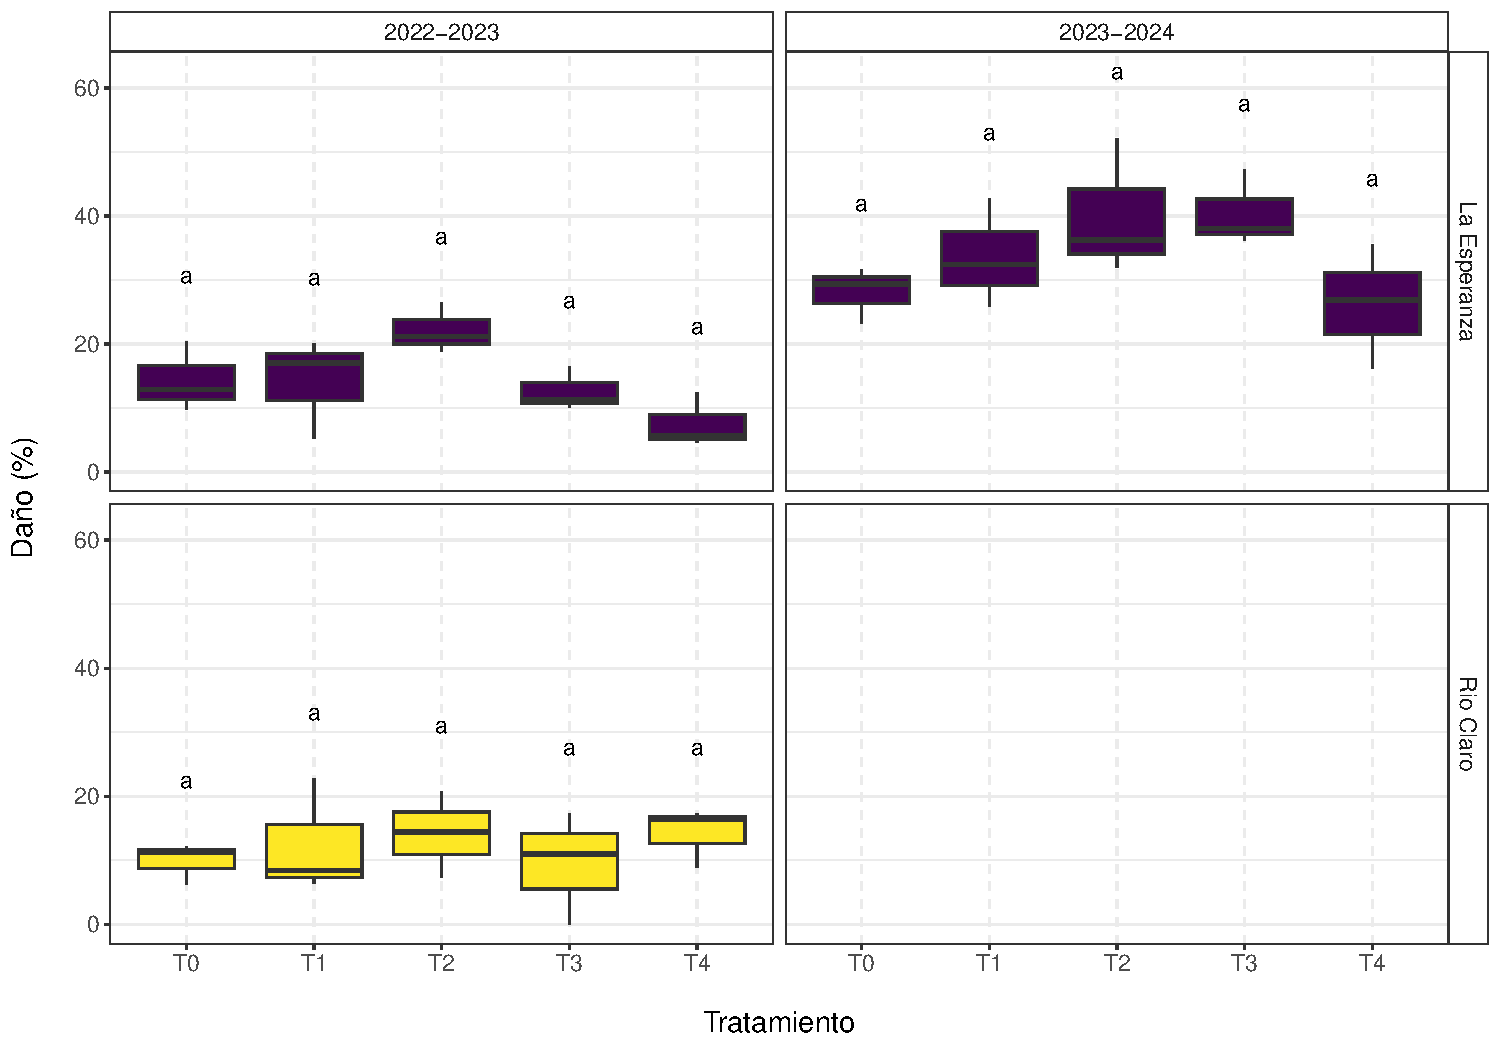
\includegraphics[keepaspectratio]{002_calidad_files/figure-pdf/unnamed-chunk-11-1.pdf}}
\end{center}

\part{Variables meteorológicas}

\chapter{Riego}\label{riego}

El gráfico muestra la lámina de agua acumulada correspondiente a la
evapotranspiración de referencia (ET₀) y al riego aplicado en cada
tratamiento durante las temporadas 2022-2023 y 2023-2024 en ambos
sitios. Las estrategias de riego con déficit hídrico (RDC) redujeron
significativamente el volumen de agua aplicada en comparación con el
riego del productor local (T0). En la temporada 2022-2023, T0 alcanzó el
83\% y 47\% de la ET₀ en Rio Claro y La Esperanza, respectivamente. Para
los tratamientos con restricción hídrica, en Rio Claro, T1 recibió el
61\% de la ET₀, T2 el 47\%, T3 el 34\% y T4 el 21\%, mientras que en La
Esperanza, T1 recibió el 47\%, T2 el 29\%, T3 el 11\% y T4 solo el 6\%.
En 2023-2024, T0 representó el 65\% y 46\% de la ET₀ en Rio Claro y La
Esperanza, respectivamente. En Rio Claro, los tratamientos T1 a T4
alcanzaron el 31\%, 21\%, 16\% y 10\% de la ET₀, mientras que en La
Esperanza no se aplicó riego en estos tratamientos debido a la falta de
impacto observado en la temporada anterior.

\pandocbounded{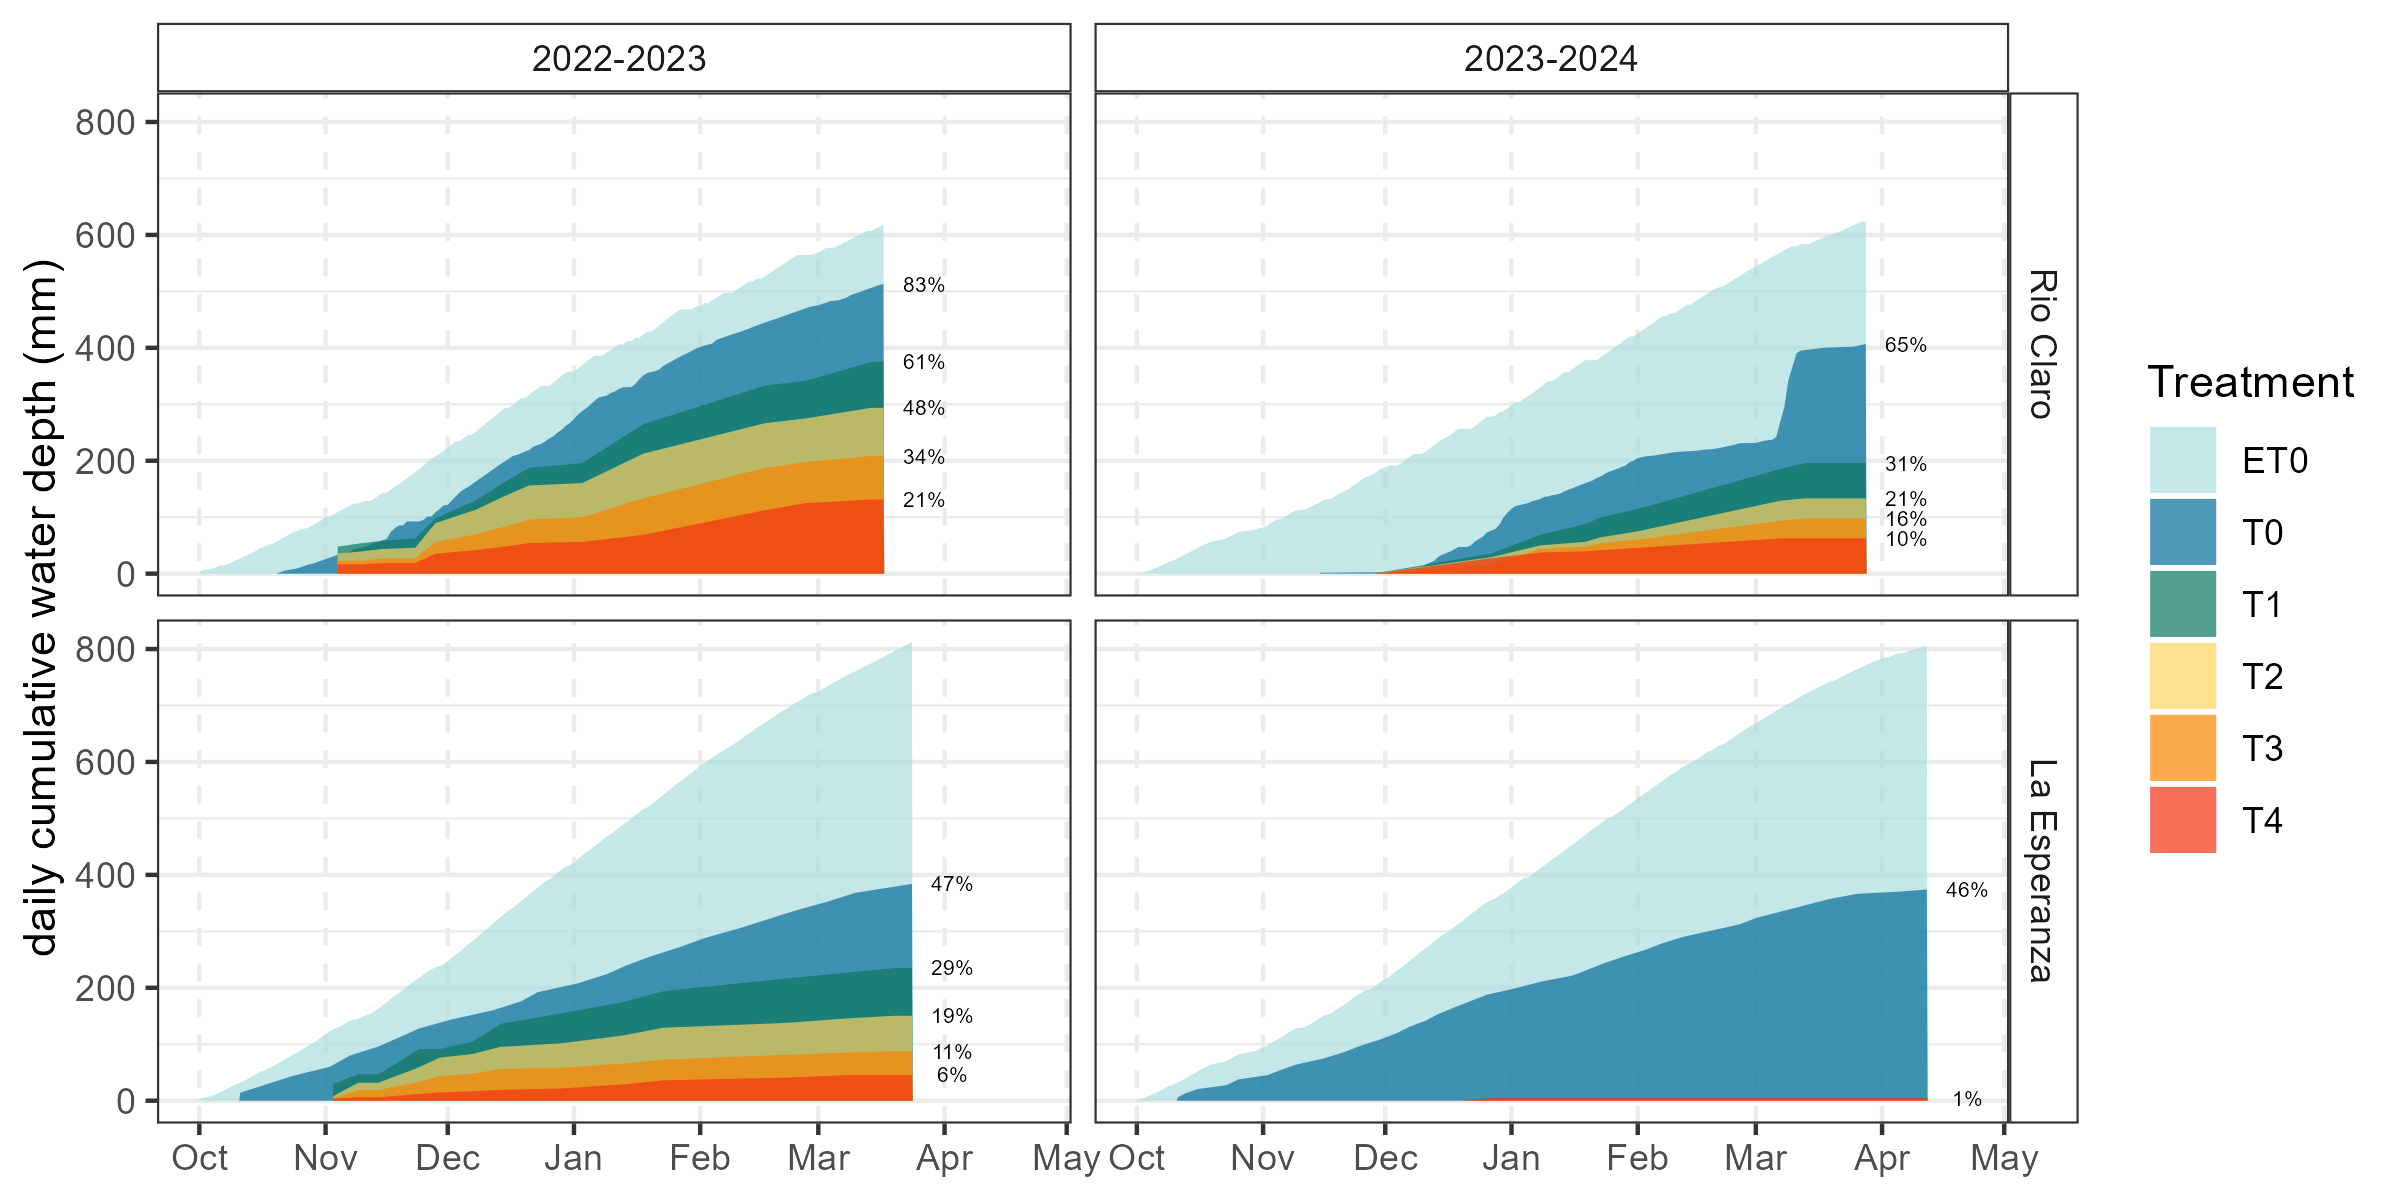
\includegraphics[keepaspectratio]{figuras/misc/riego_lamina.png}}

\chapter{Clima}\label{clima}

Las variables climáticas fueron obtenidas de las estaciones
meteorológicas de Garces Fruits ubicadas en ambos sitios.

\chapter{Temperatura}

\begin{center}
\pandocbounded{\includegraphics[keepaspectratio]{004_clima_files/figure-pdf/unnamed-chunk-3-1.pdf}}
\end{center}

\chapter{Déficit de presión de vapor (VPD)}

\begin{center}
\pandocbounded{\includegraphics[keepaspectratio]{004_clima_files/figure-pdf/unnamed-chunk-4-1.pdf}}
\end{center}

\chapter{Evapotranspiración de referencia (ET0)}

\begin{center}
\pandocbounded{\includegraphics[keepaspectratio]{004_clima_files/figure-pdf/unnamed-chunk-5-1.pdf}}
\end{center}

\chapter{Precipitación}

\begin{center}
\pandocbounded{\includegraphics[keepaspectratio]{004_clima_files/figure-pdf/unnamed-chunk-6-1.pdf}}
\end{center}

\chapter{Humedad de suelo}\label{humedad-de-suelo}

\chapter{Por tratamiento}

\begin{center}
\pandocbounded{\includegraphics[keepaspectratio]{005_humedad_files/figure-pdf/unnamed-chunk-1-1.pdf}}
\end{center}

\chapter{Por temporada}

\begin{center}
\pandocbounded{\includegraphics[keepaspectratio]{005_humedad_files/figure-pdf/unnamed-chunk-2-1.pdf}}
\end{center}

\chapter{Serie temporal 2022-2023}

\begin{center}
\pandocbounded{\includegraphics[keepaspectratio]{005_humedad_files/figure-pdf/unnamed-chunk-3-1.pdf}}
\end{center}

\chapter{Serie temporal 2023-2024}

\begin{center}
\pandocbounded{\includegraphics[keepaspectratio]{005_humedad_files/figure-pdf/unnamed-chunk-4-1.pdf}}
\end{center}

\part{Parámetros fisiológicos}

\chapter{Parámetros fisiológicos}\label{paruxe1metros-fisioluxf3gicos-1}

\section{Fluorescencia}\label{fluorescencia}

\chapter{Por tratamiento}

\begin{center}
\pandocbounded{\includegraphics[keepaspectratio]{006_parametros_files/figure-pdf/unnamed-chunk-2-1.pdf}}
\end{center}

\chapter{Por temporada}

\begin{center}
\pandocbounded{\includegraphics[keepaspectratio]{006_parametros_files/figure-pdf/unnamed-chunk-3-1.pdf}}
\end{center}

\chapter{Series temporales}

\pandocbounded{\includegraphics[keepaspectratio]{006_parametros_files/figure-pdf/unnamed-chunk-4-1.pdf}}

\section{Potencial}\label{potencial}

\chapter{Por tratamiento}

\begin{center}
\pandocbounded{\includegraphics[keepaspectratio]{006_parametros_files/figure-pdf/unnamed-chunk-5-1.pdf}}
\end{center}

\chapter{Por temporada}

\begin{center}
\pandocbounded{\includegraphics[keepaspectratio]{006_parametros_files/figure-pdf/unnamed-chunk-6-1.pdf}}
\end{center}

\chapter{Serie temporal}

\begin{center}
\pandocbounded{\includegraphics[keepaspectratio]{006_parametros_files/figure-pdf/unnamed-chunk-7-1.pdf}}
\end{center}

\section{LAI}\label{lai}

\chapter{Por tratamiento}

\begin{center}
\pandocbounded{\includegraphics[keepaspectratio]{006_parametros_files/figure-pdf/unnamed-chunk-8-1.pdf}}
\end{center}

\chapter{Por temporada}

\begin{center}
\pandocbounded{\includegraphics[keepaspectratio]{006_parametros_files/figure-pdf/unnamed-chunk-9-1.pdf}}
\end{center}

\chapter{Serie temporal}

\begin{center}
\pandocbounded{\includegraphics[keepaspectratio]{006_parametros_files/figure-pdf/unnamed-chunk-10-1.pdf}}
\end{center}

\chapter{Punto de pérdida de
turgor}\label{punto-de-puxe9rdida-de-turgor}

A continuación se presentan los puntos de pérdida de turgor de cada
unidad, según tratamiento, sitio y temporada, a partir de las curvas
presión-volumen, como se describe en el anexo
\href{https://mherreradiaz.github.io/reporte_general/static/anexos/pv_metodology.html}{Curvas
Presión-Volumen}.

\begin{center}
\pandocbounded{\includegraphics[keepaspectratio]{007_tlp_files/figure-pdf/unnamed-chunk-1-1.pdf}}
\end{center}

\part{Preprocesamiento de datos de turgor}

Para el preprocesamiento de los datos se llevó a cabo una limpieza
basada en clustering y la correlación con la temperatura y VPD. Esto
permitió diferenciar periodos que se alejaban del comportamiento normal
del turgor (i.e.~puntos máximos a la hora de más demanda hídrica del día
y disminución en las horas de la noche). A continuación se presenta el
diagrama de flujo del preprocesamiento de los datos de turgor.

\includegraphics[width=6.1in,height=9.81in]{100_preproceso_turgor_files/figure-latex/mermaid-figure-1.png}

\chapter{Clustering}\label{clustering}

{[}Metodología de clustering{]}.

A continuación, se muestran las series temporales de turgor
diferenciadas por clúster, así como la distribución de las horas de
turgor mínimo y máximo para cada uno de ellos, junto con su ciclo
horario diario, abarcando todos los sensores en todas las unidades
durante las temporadas 2022-2023 y 2023-2024.

\section{La Esperanza}\label{la-esperanza}

\chapter{T1 (2022-2023)}

Unidad 1
\pandocbounded{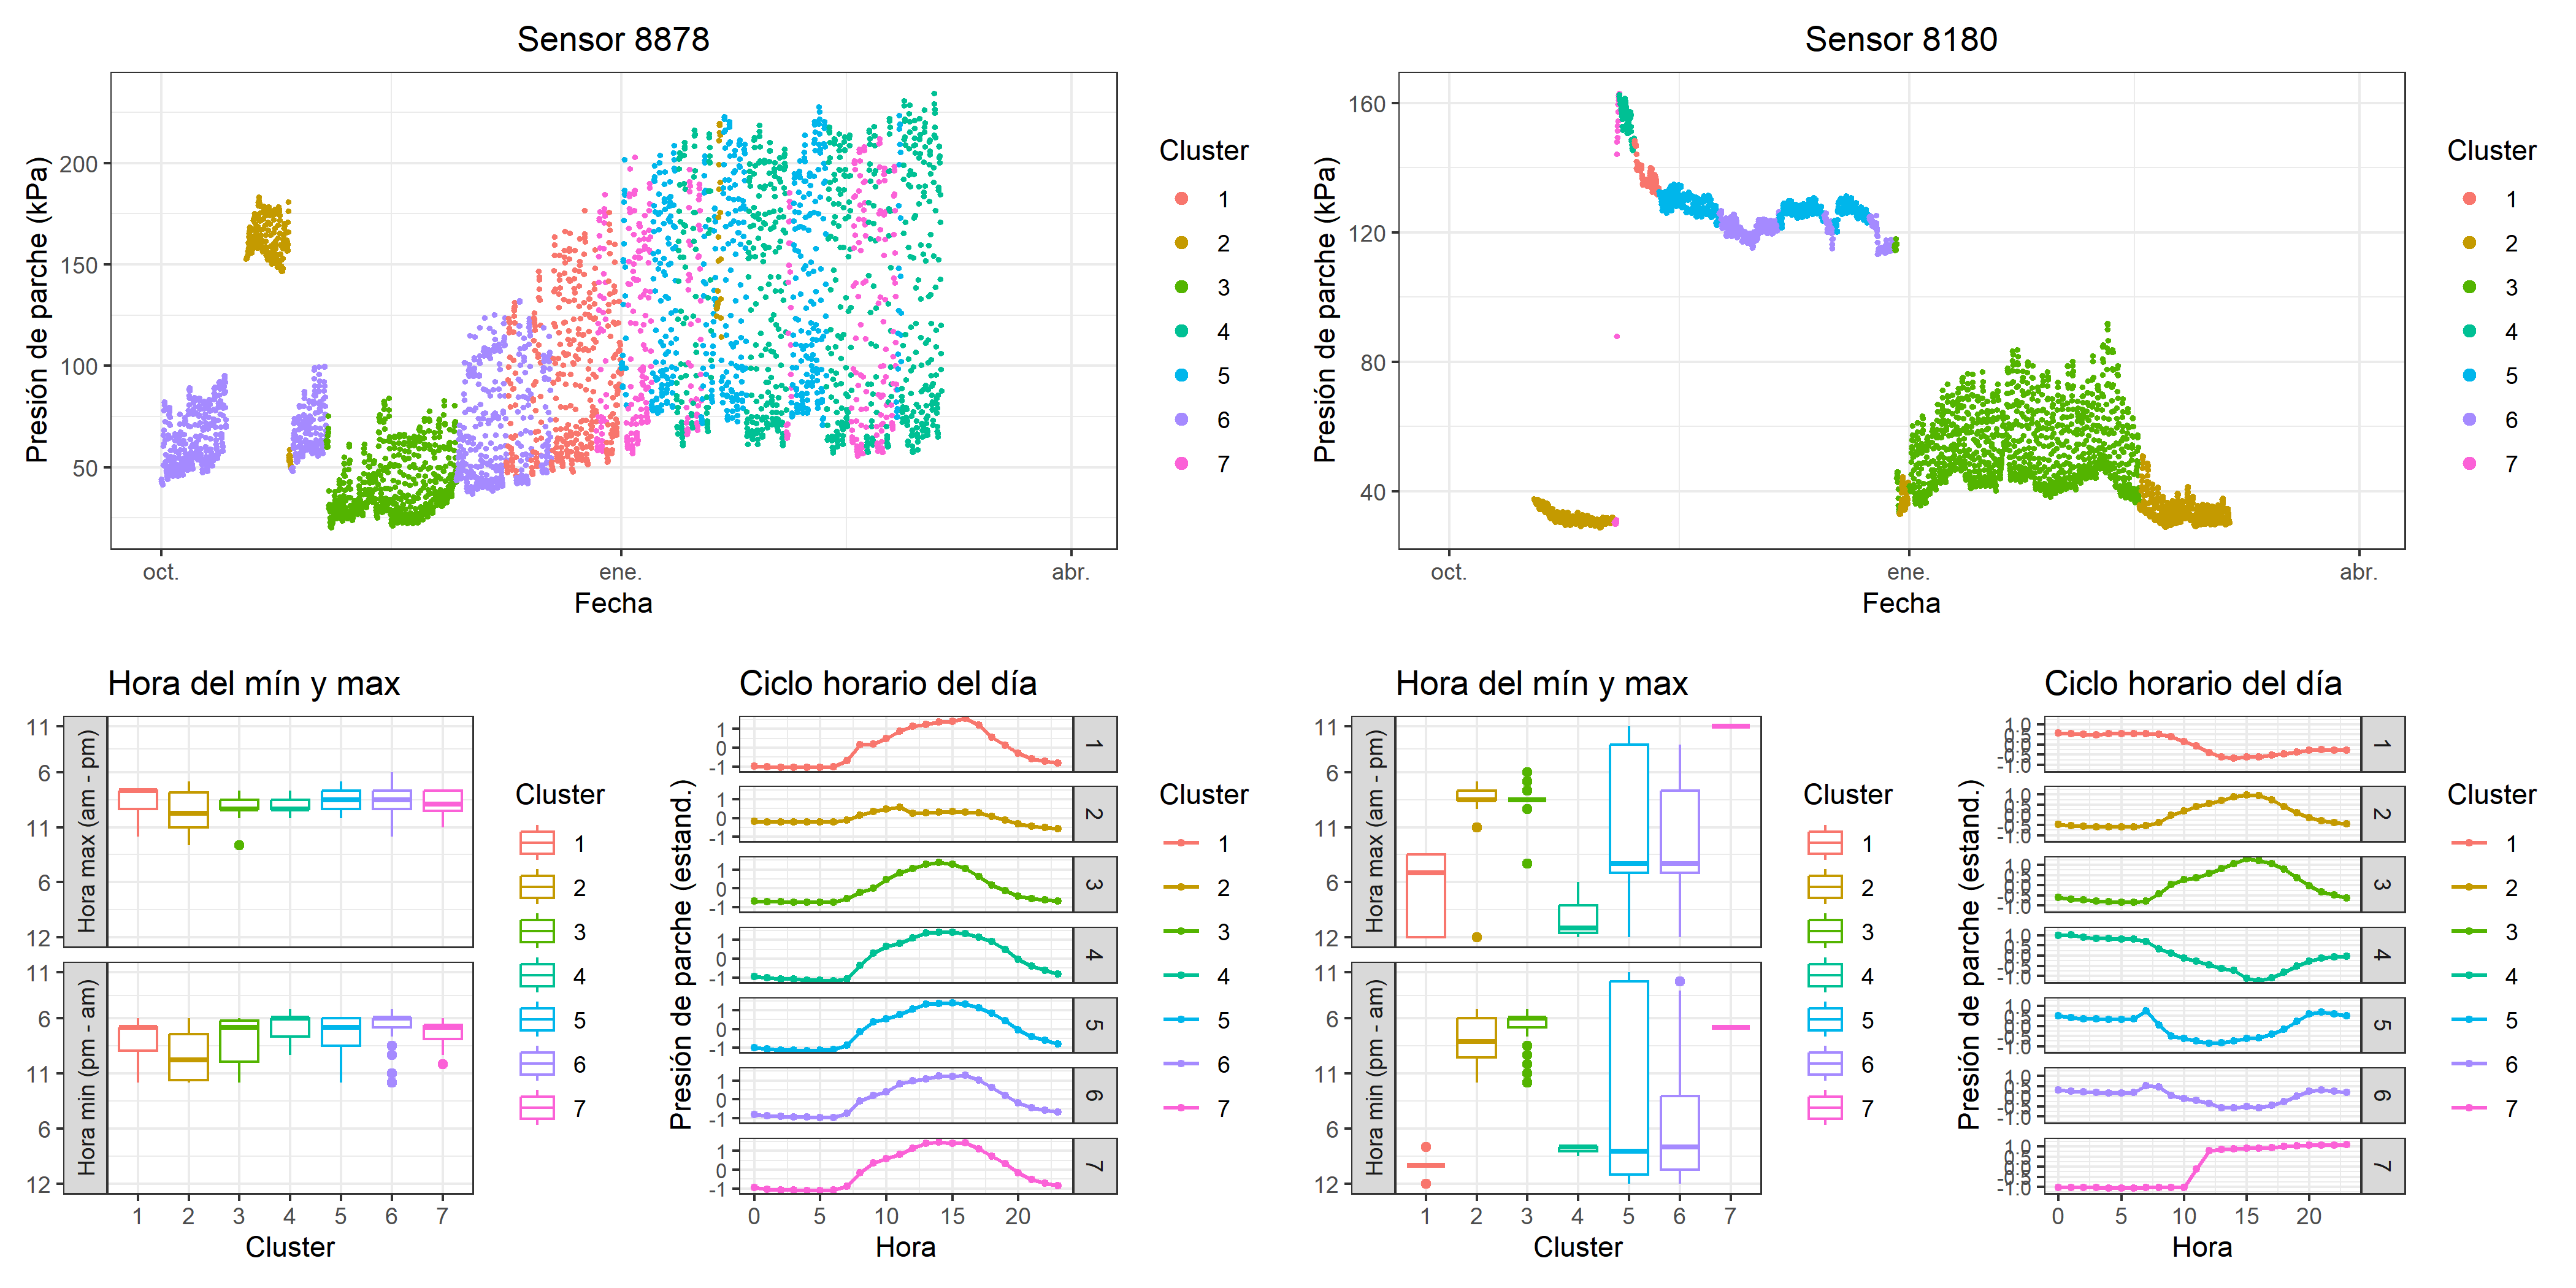
\includegraphics[keepaspectratio]{figuras/01_turgor_sensor/2022_2023_La_Esperanza_T1_Unidad_1.png}}

Unidad 2
\pandocbounded{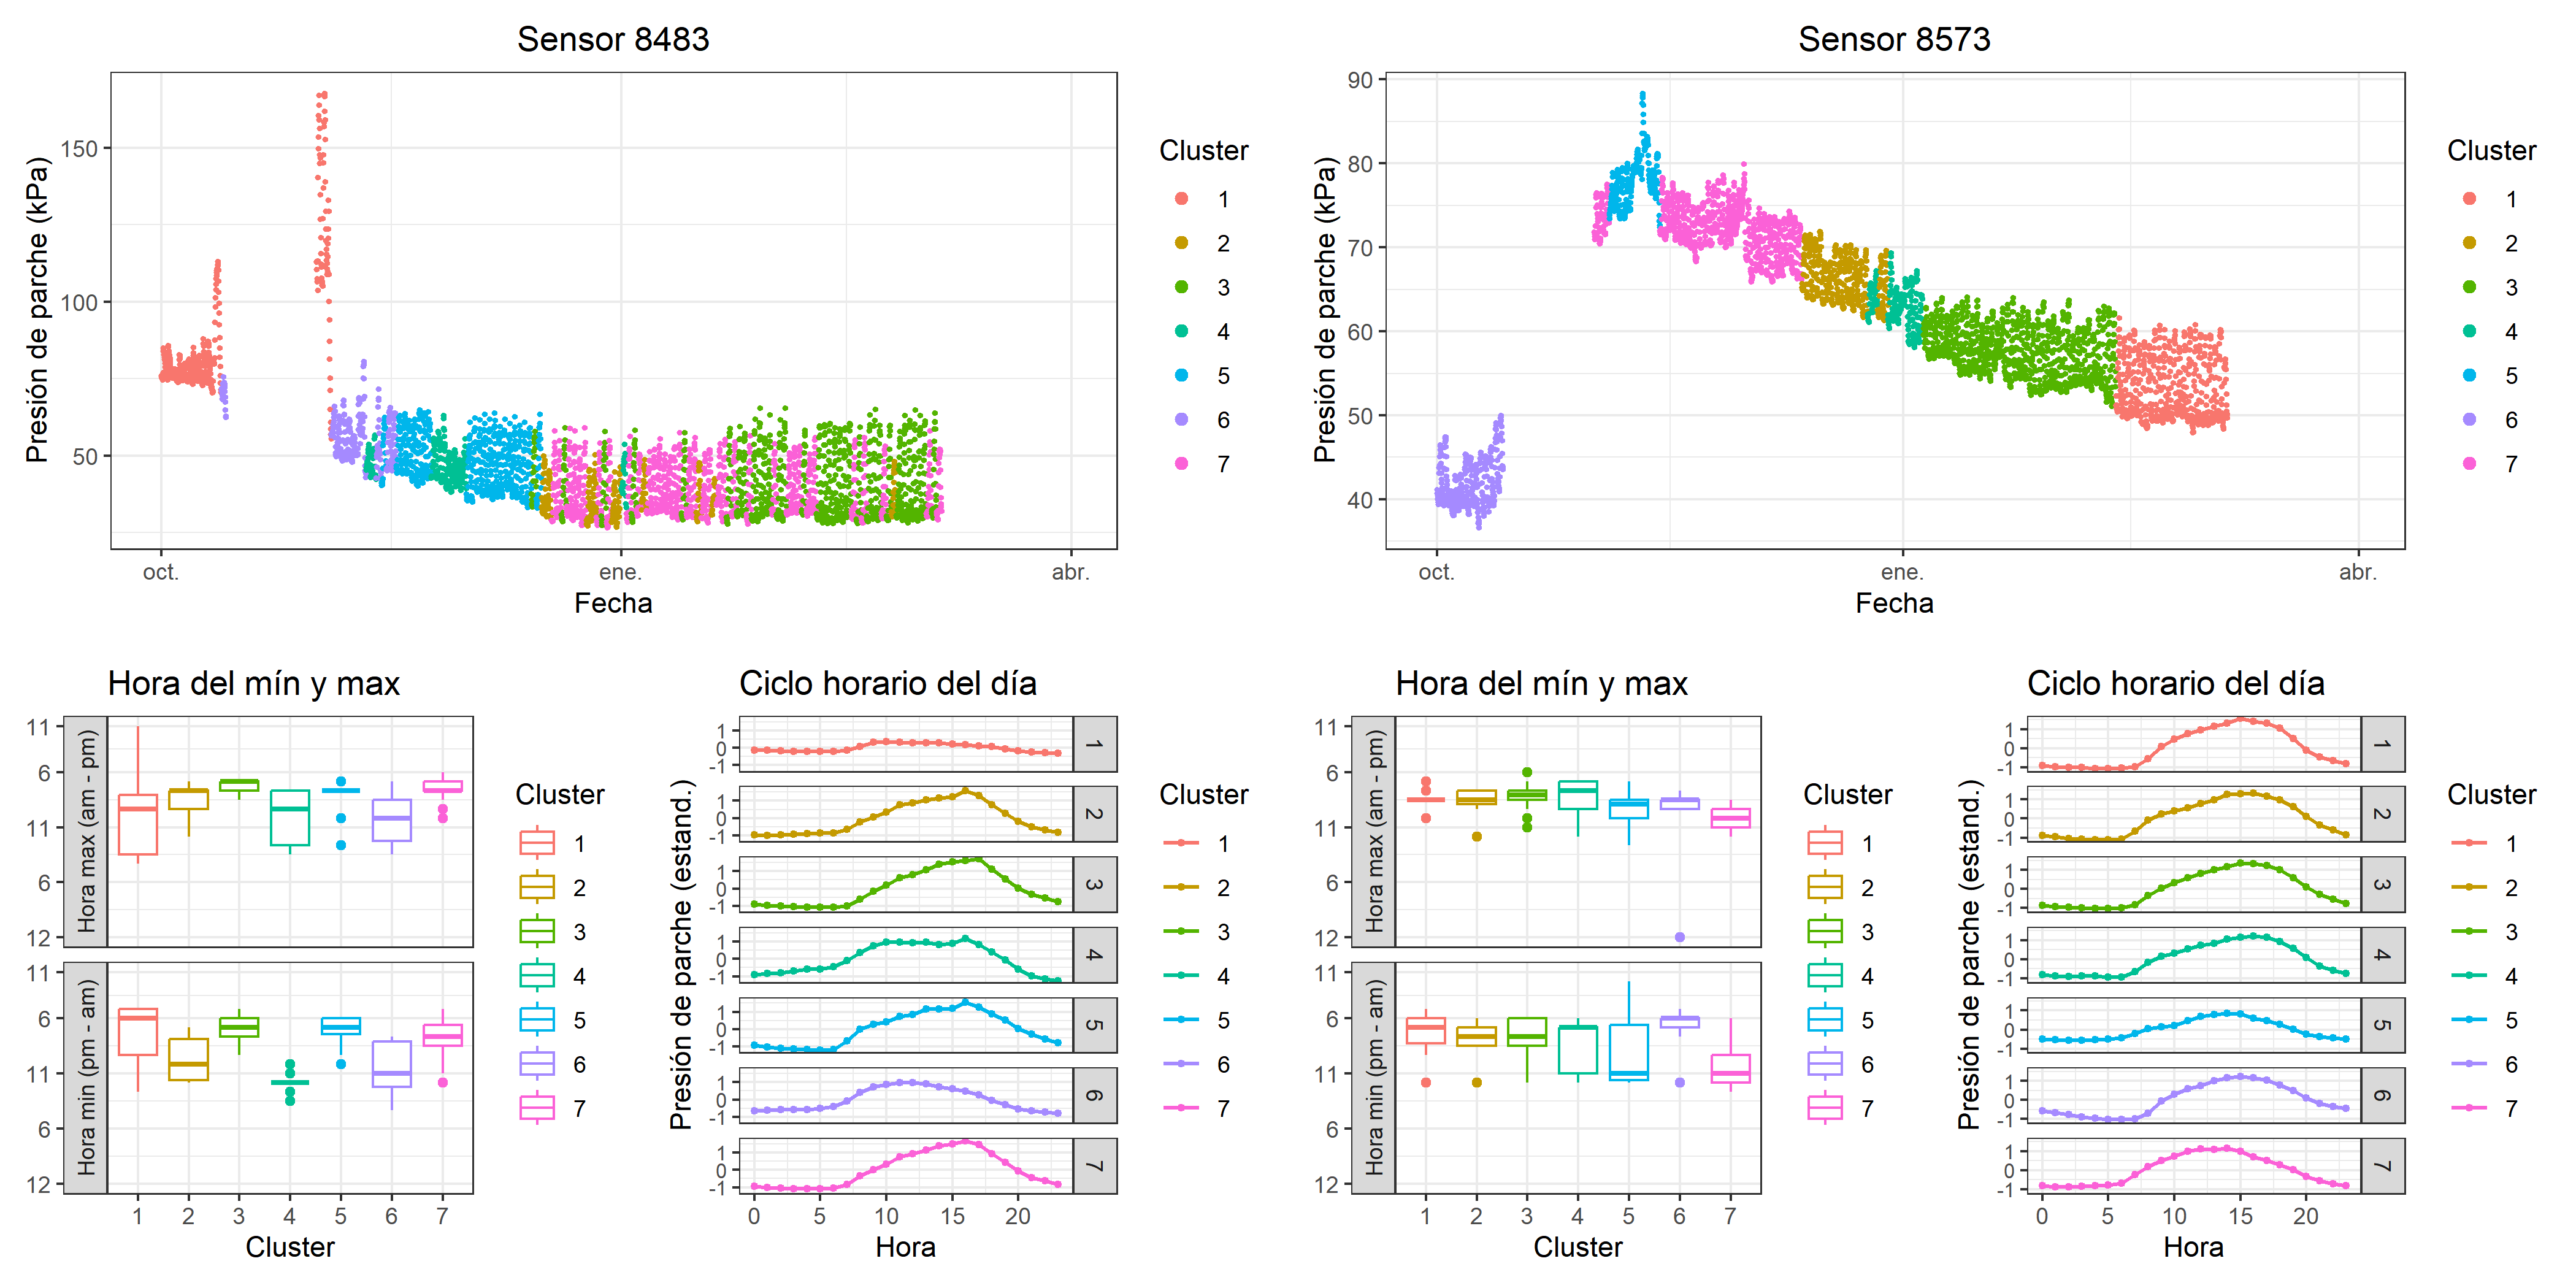
\includegraphics[keepaspectratio]{figuras/01_turgor_sensor/2022_2023_La_Esperanza_T1_Unidad_2.png}}

Unidad 3
\pandocbounded{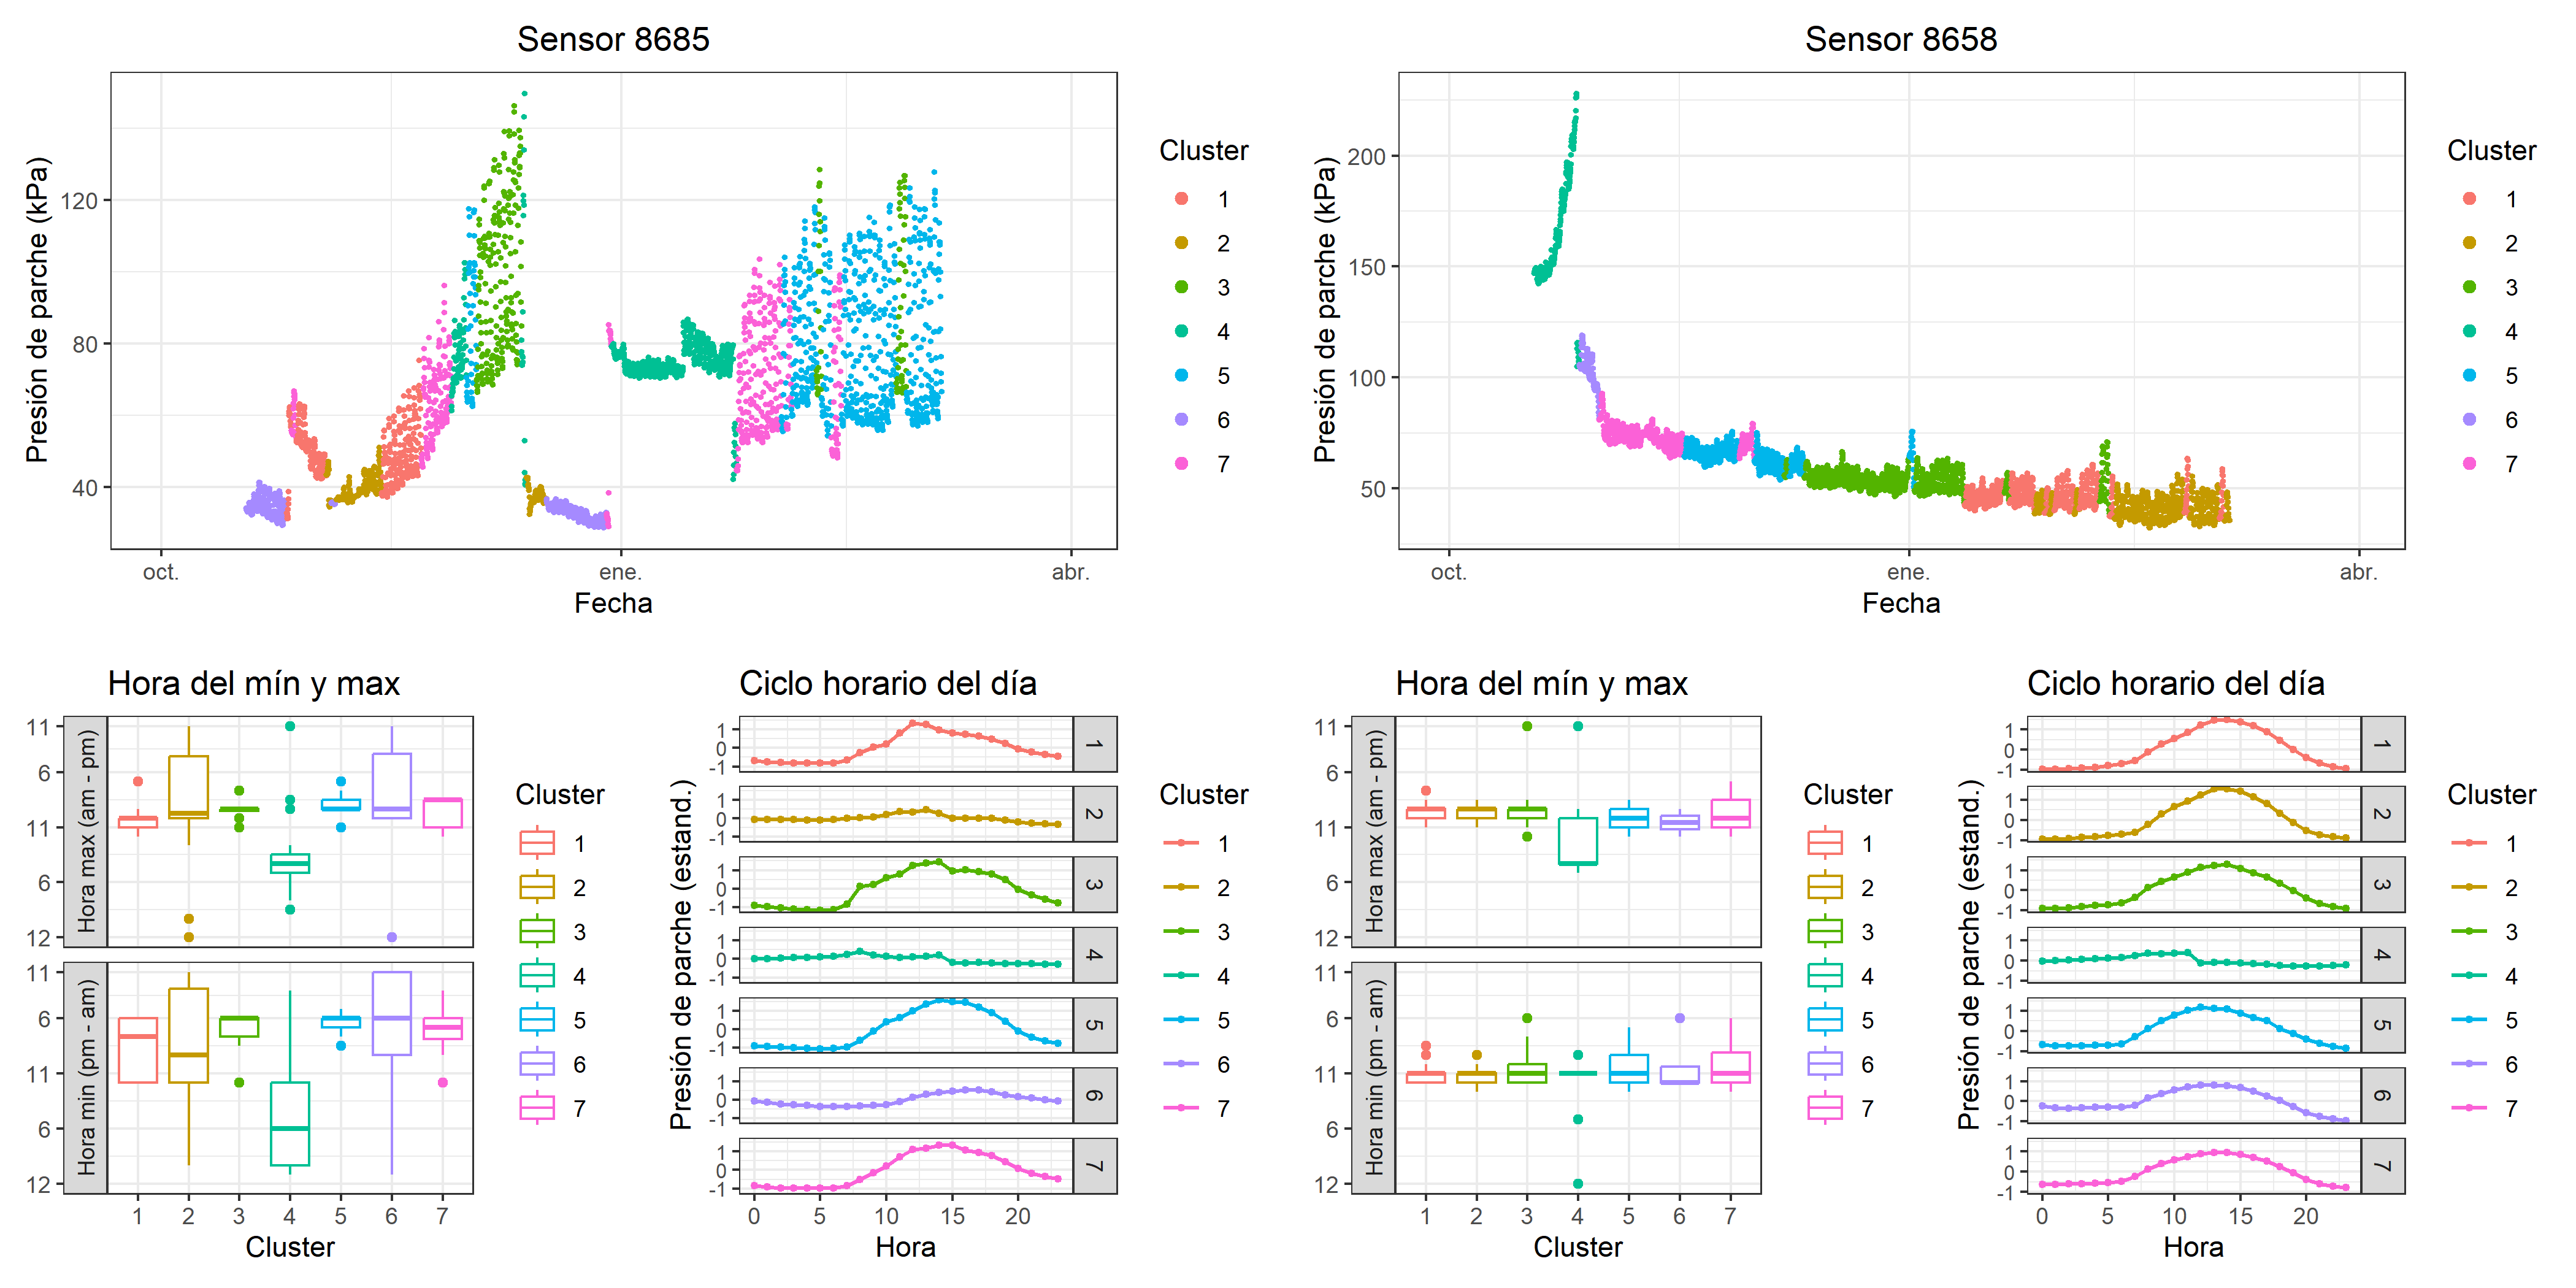
\includegraphics[keepaspectratio]{figuras/01_turgor_sensor/2022_2023_La_Esperanza_T1_Unidad_3.png}}

\chapter{T2 (2022-2023)}

Unidad 1
\pandocbounded{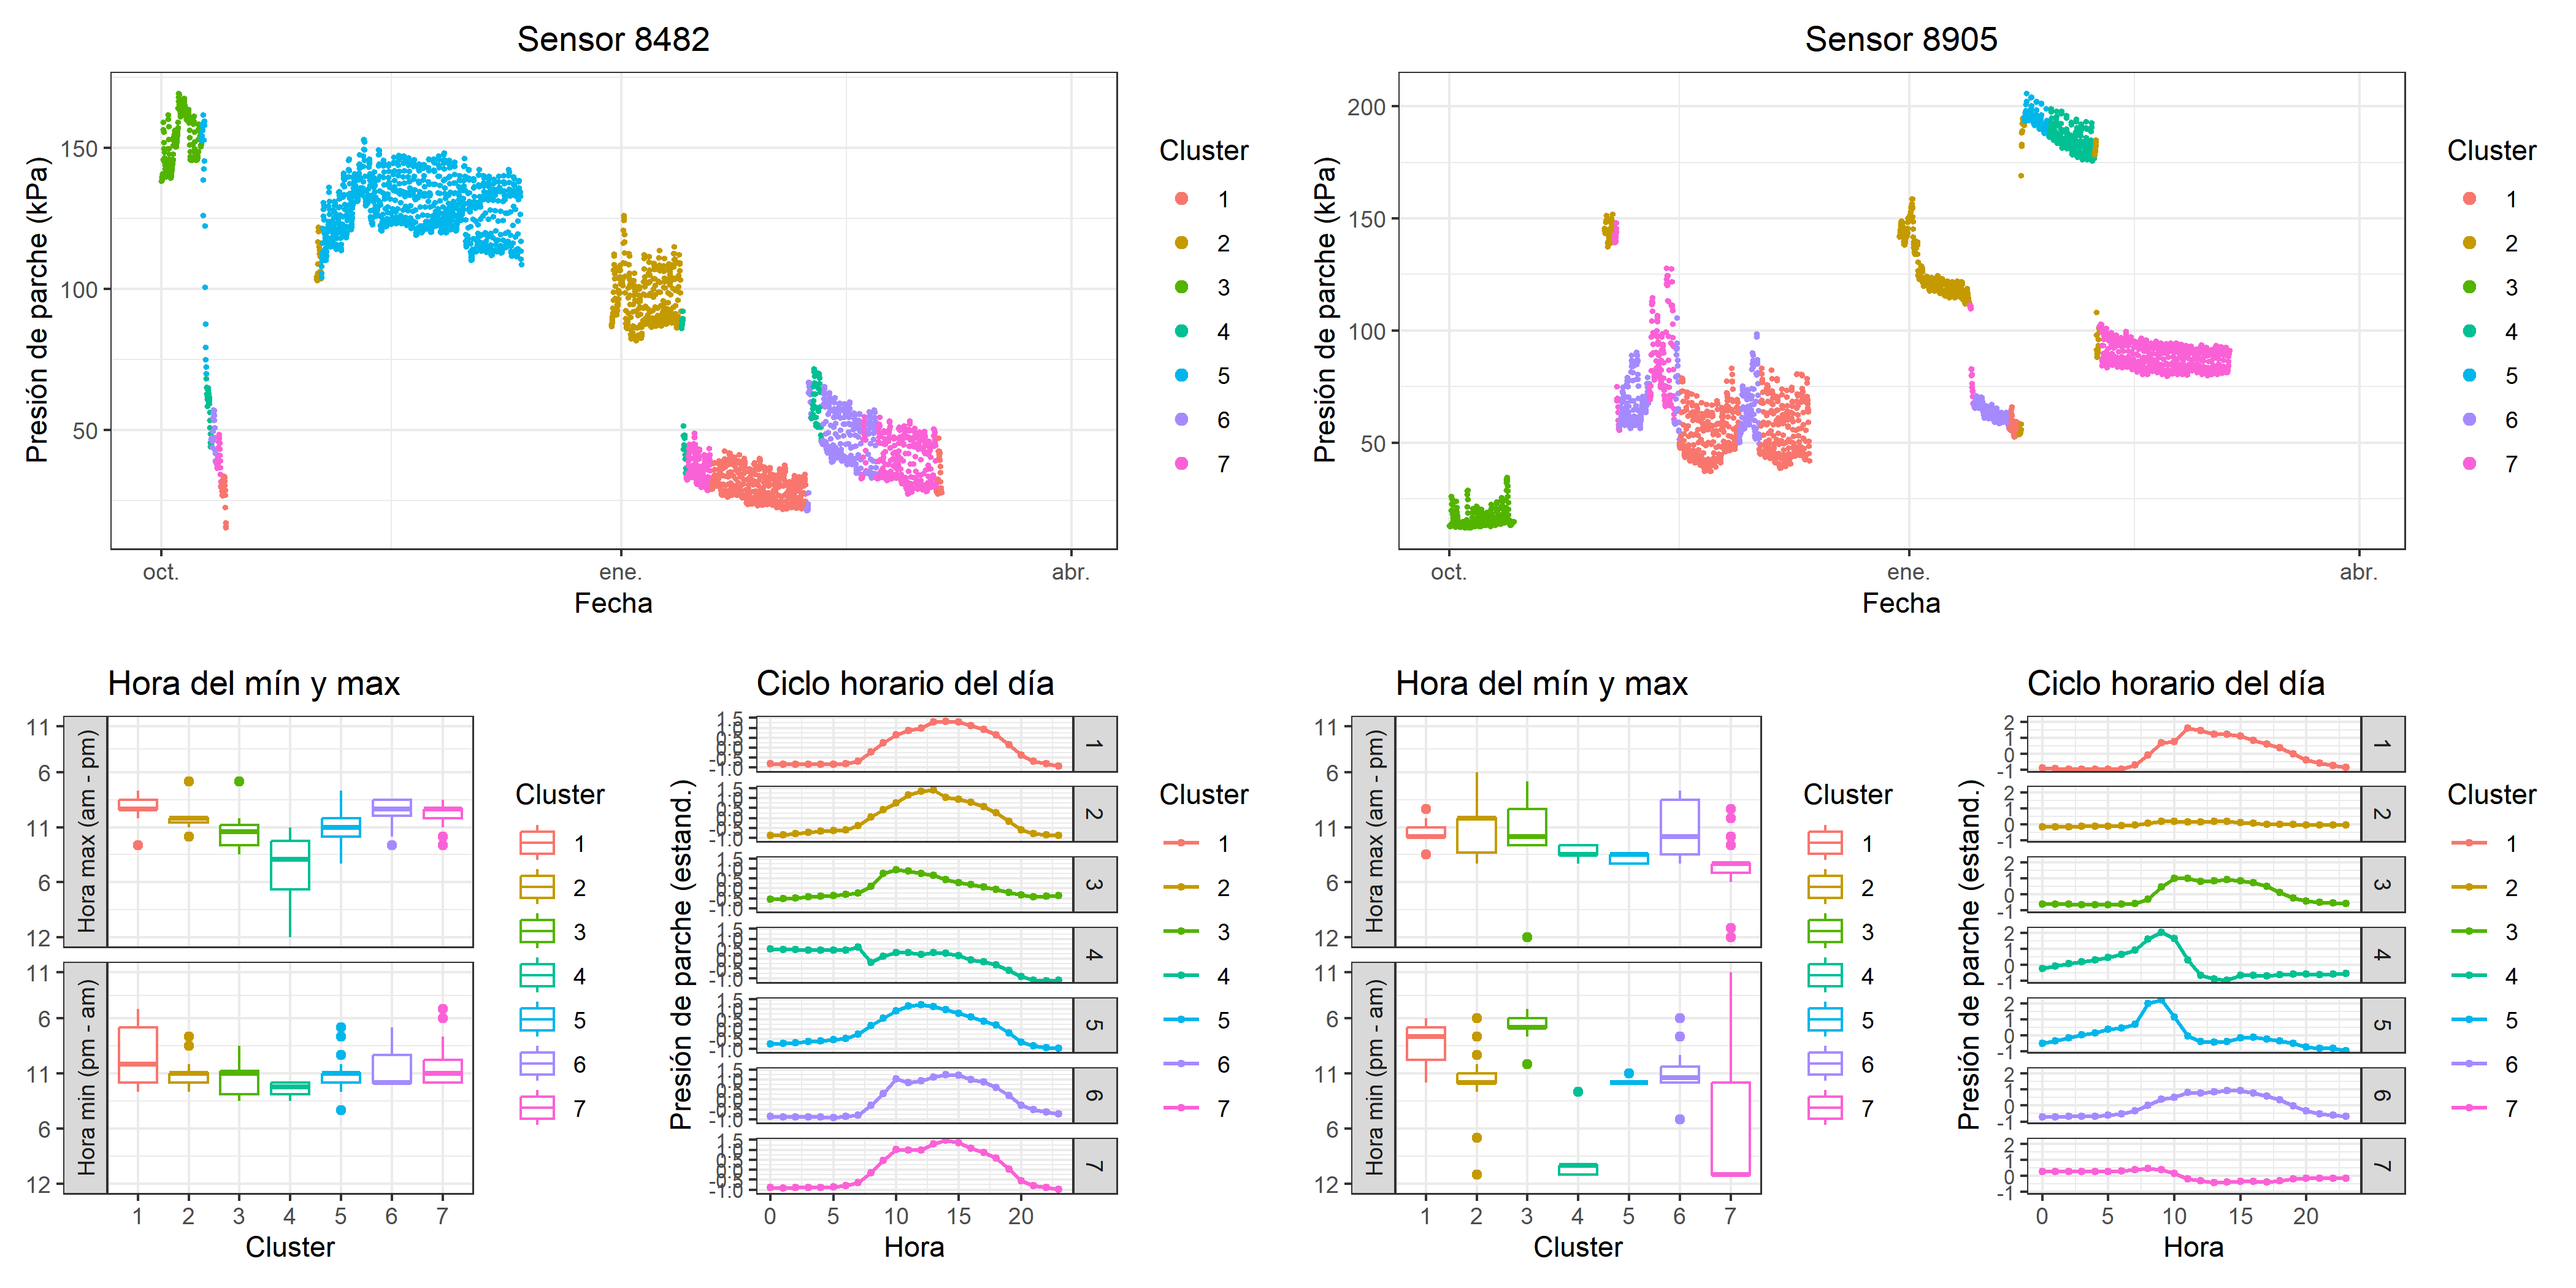
\includegraphics[keepaspectratio]{figuras/01_turgor_sensor/2022_2023_La_Esperanza_T2_Unidad_1.png}}

Unidad 2
\pandocbounded{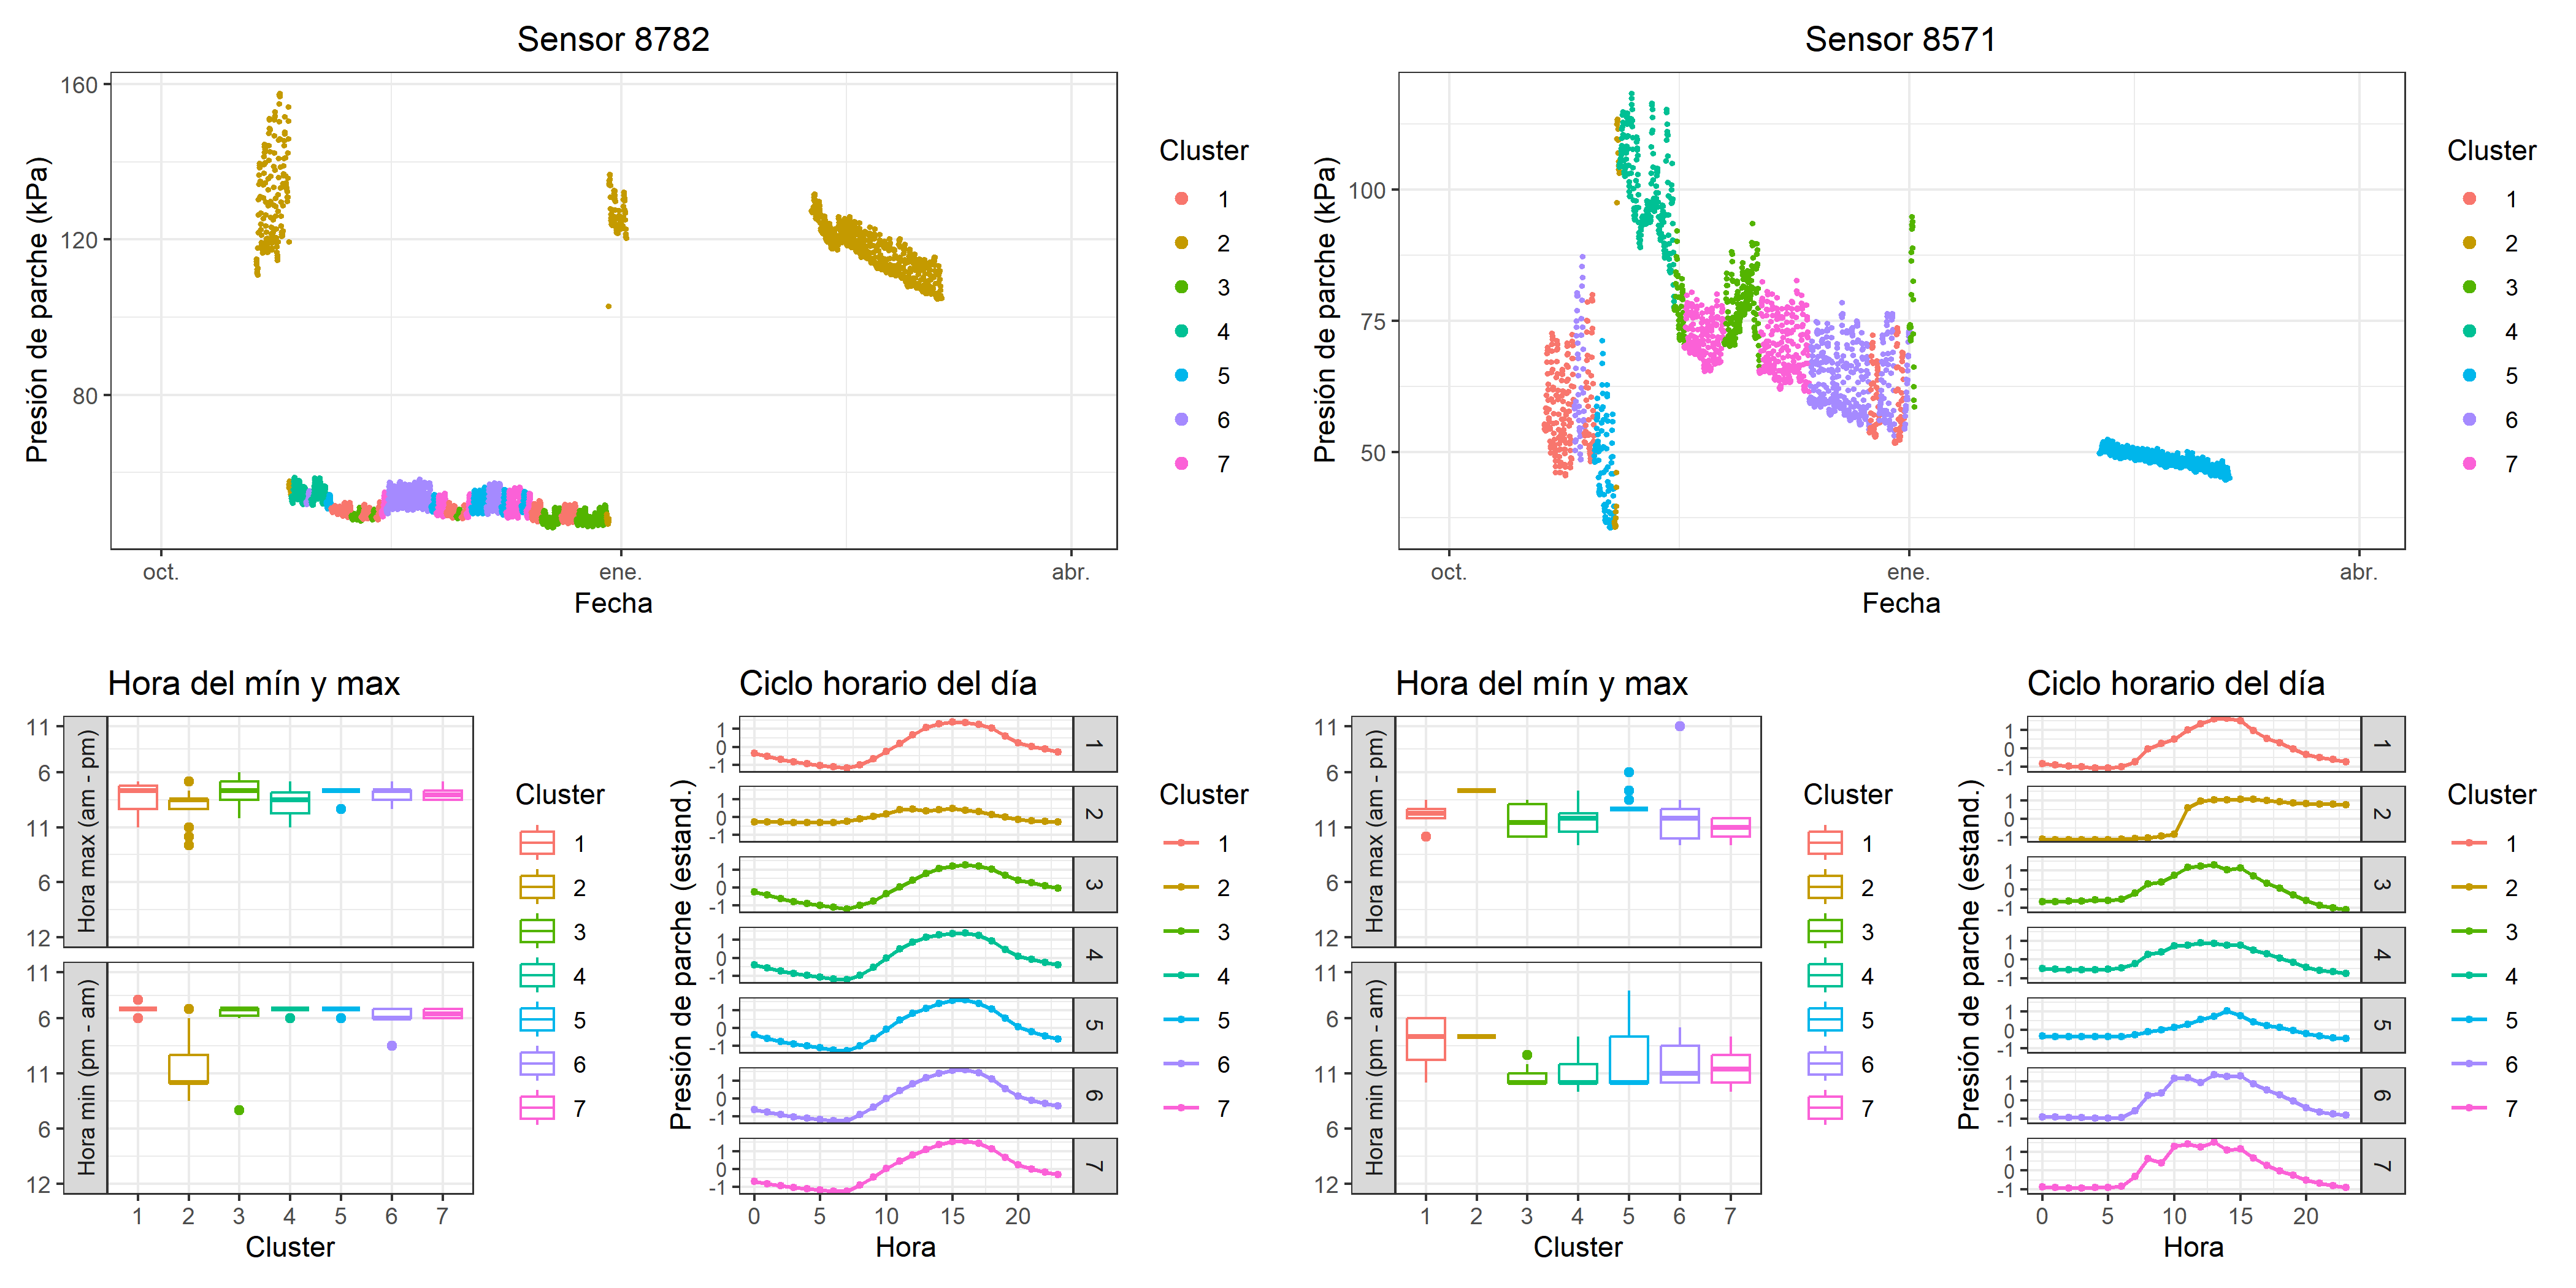
\includegraphics[keepaspectratio]{figuras/01_turgor_sensor/2022_2023_La_Esperanza_T2_Unidad_2.png}}

Unidad 3
\pandocbounded{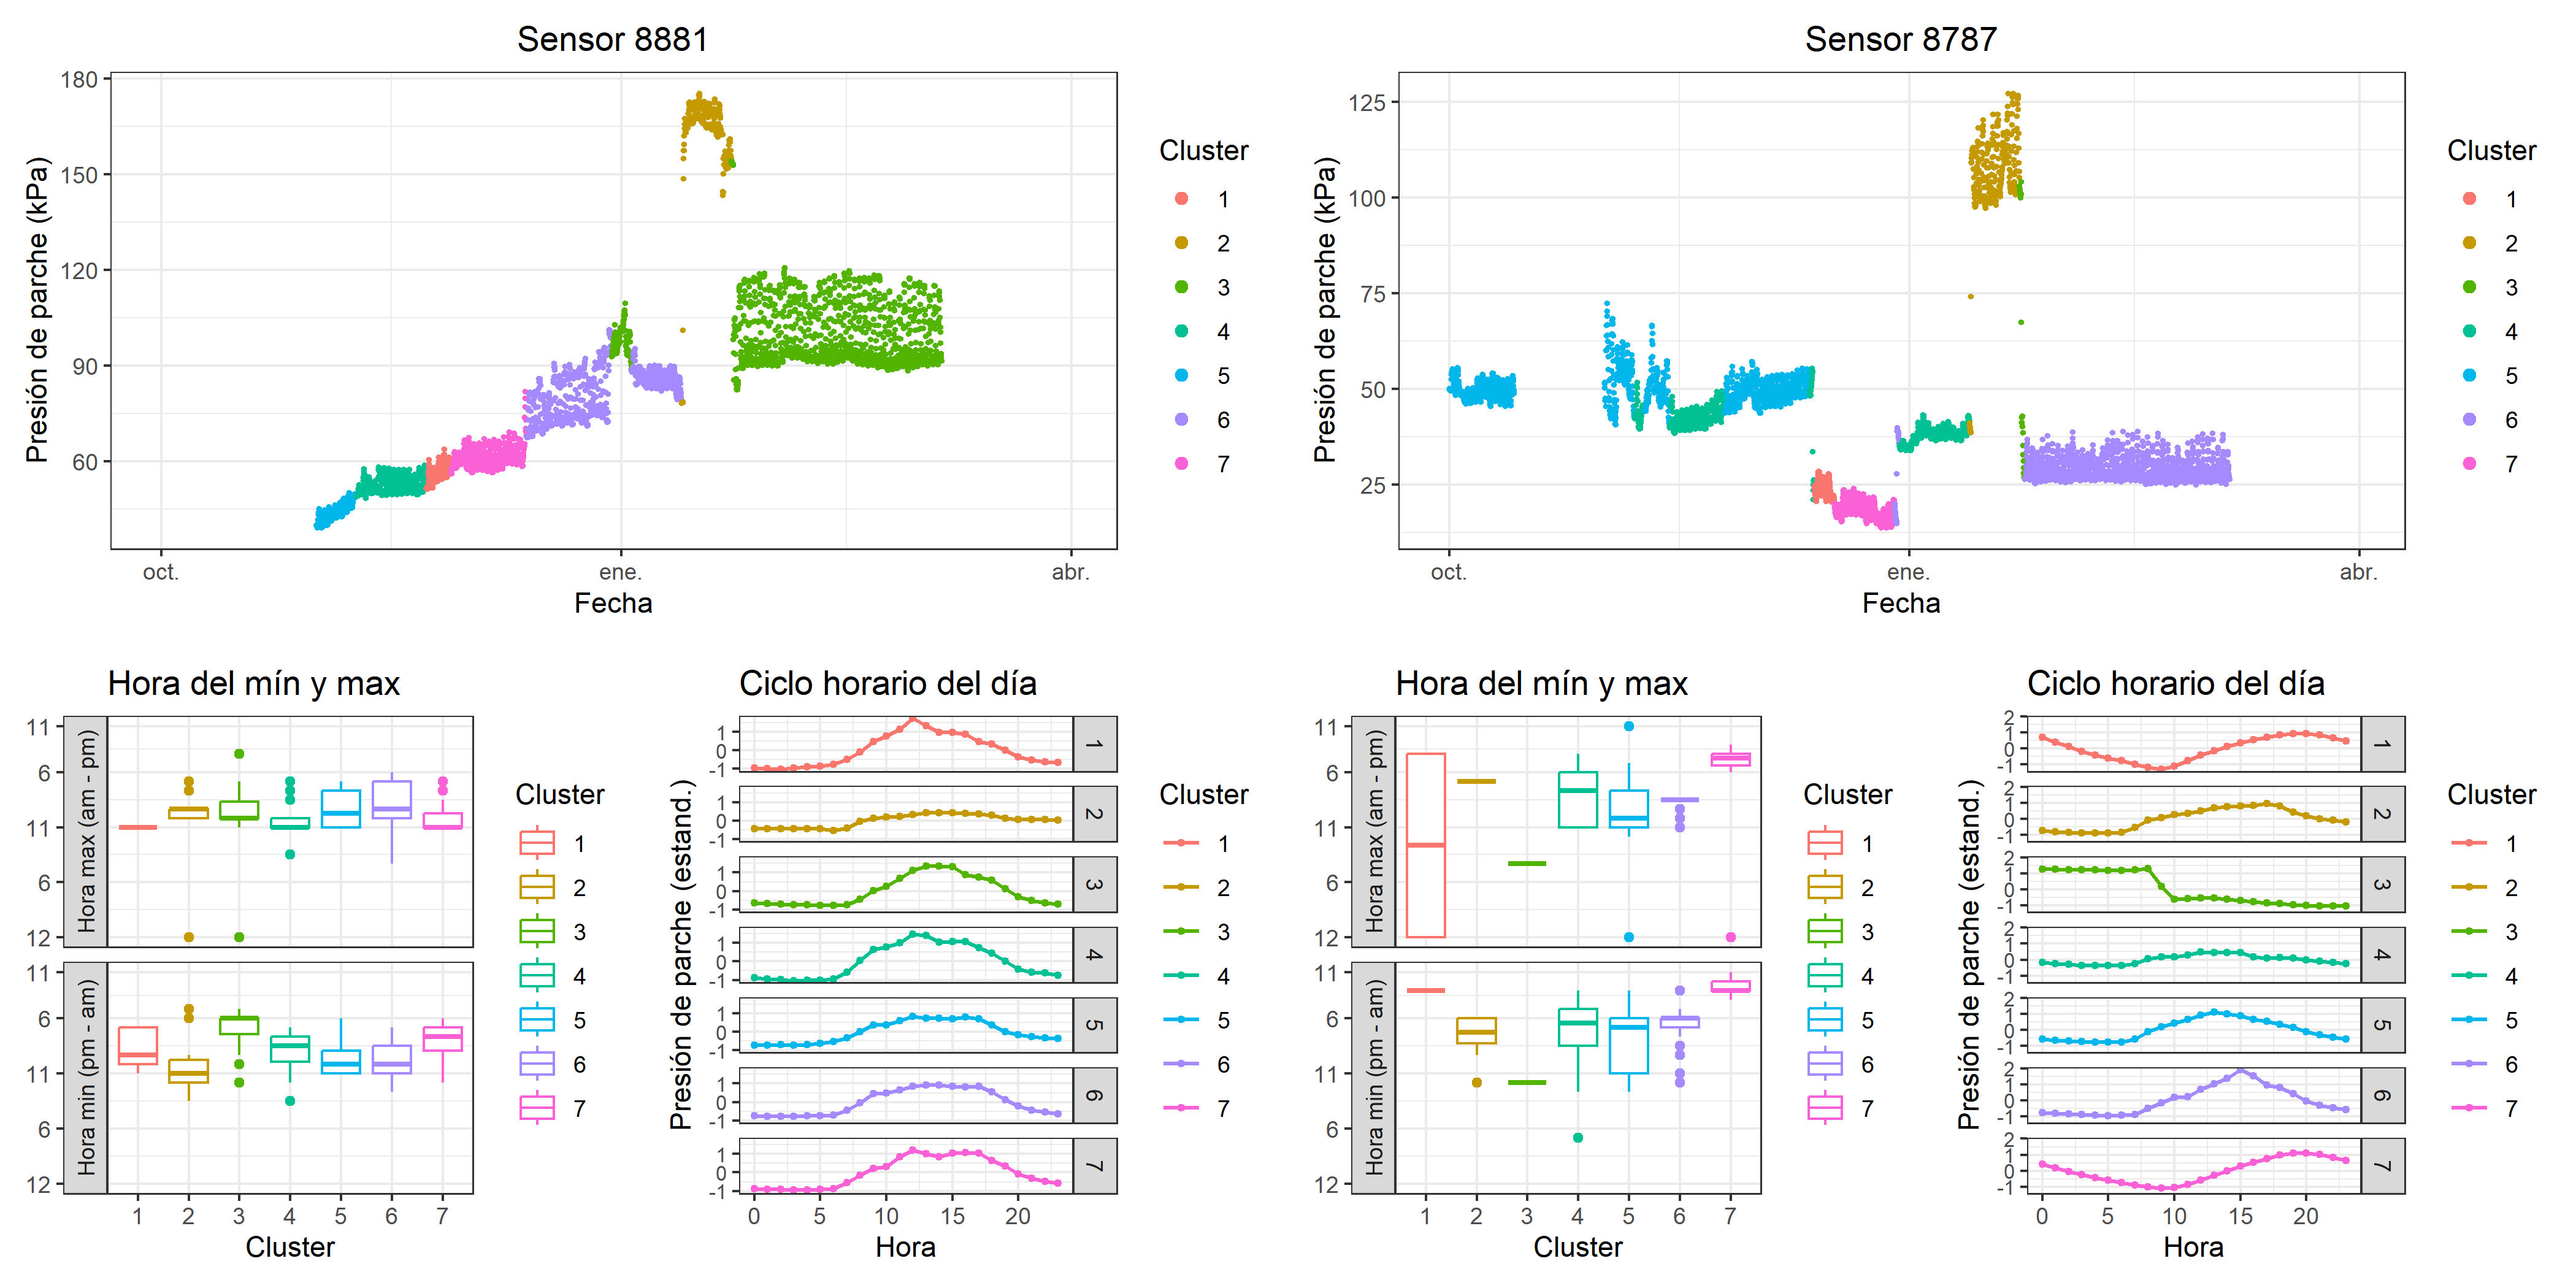
\includegraphics[keepaspectratio]{figuras/01_turgor_sensor/2022_2023_La_Esperanza_T2_Unidad_3.png}}

\chapter{T3 (2022-2023)}

Unidad 1
\pandocbounded{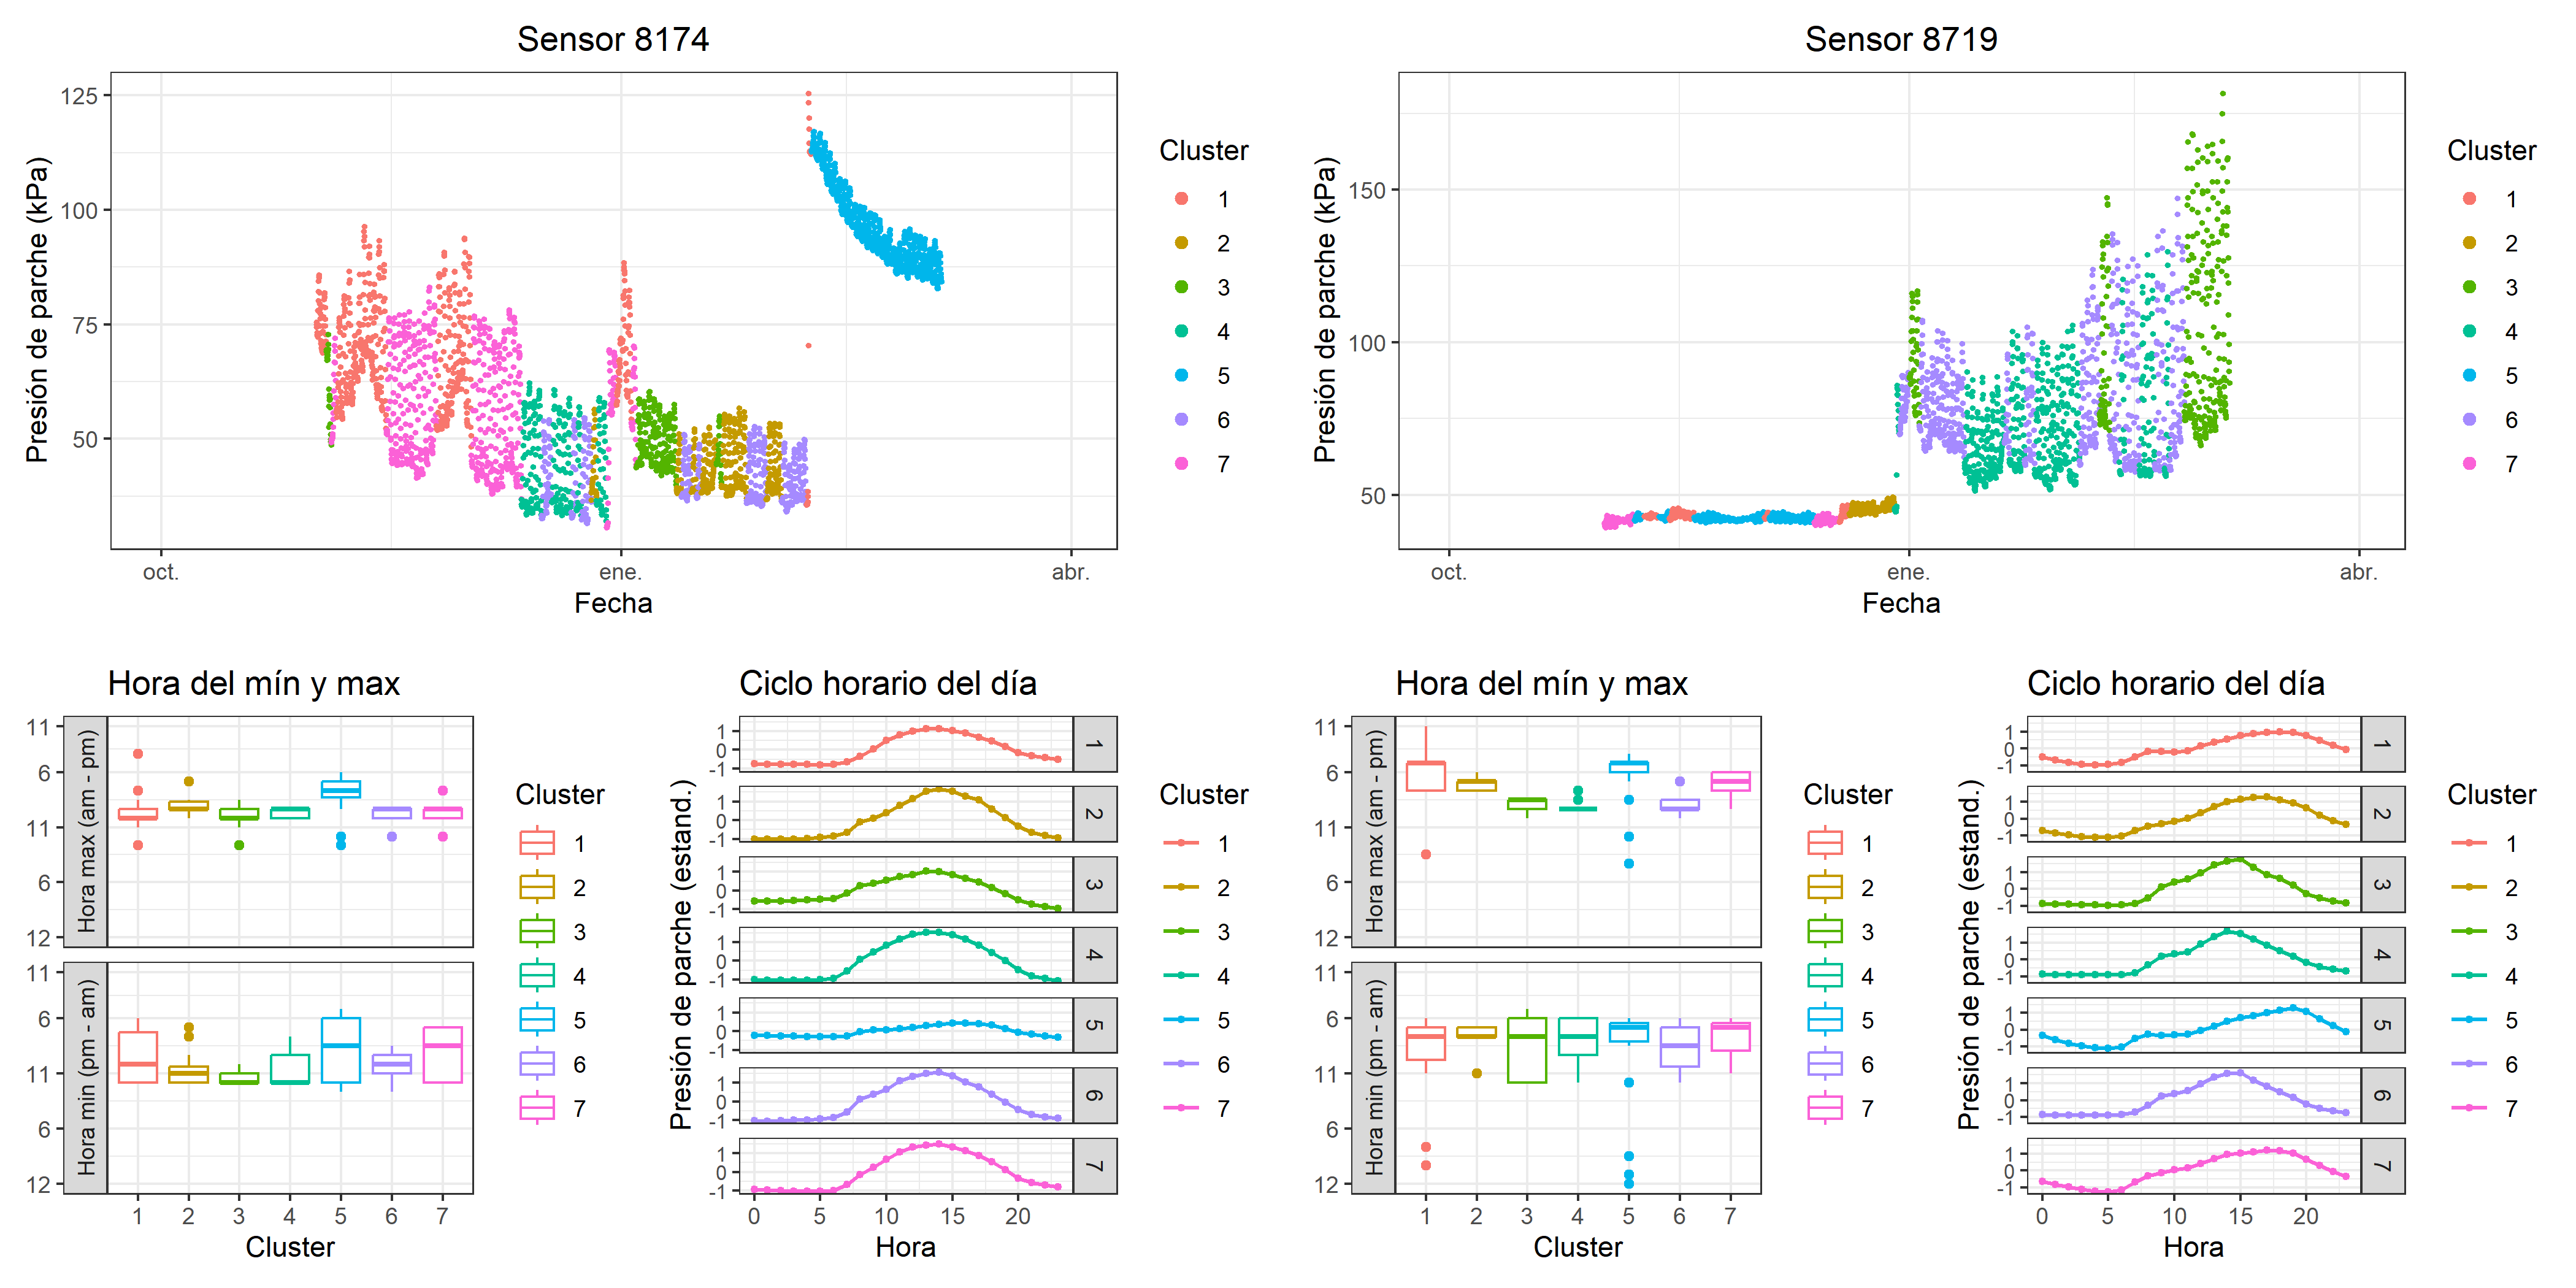
\includegraphics[keepaspectratio]{figuras/01_turgor_sensor/2022_2023_La_Esperanza_T3_Unidad_1.png}}

Unidad 2
\pandocbounded{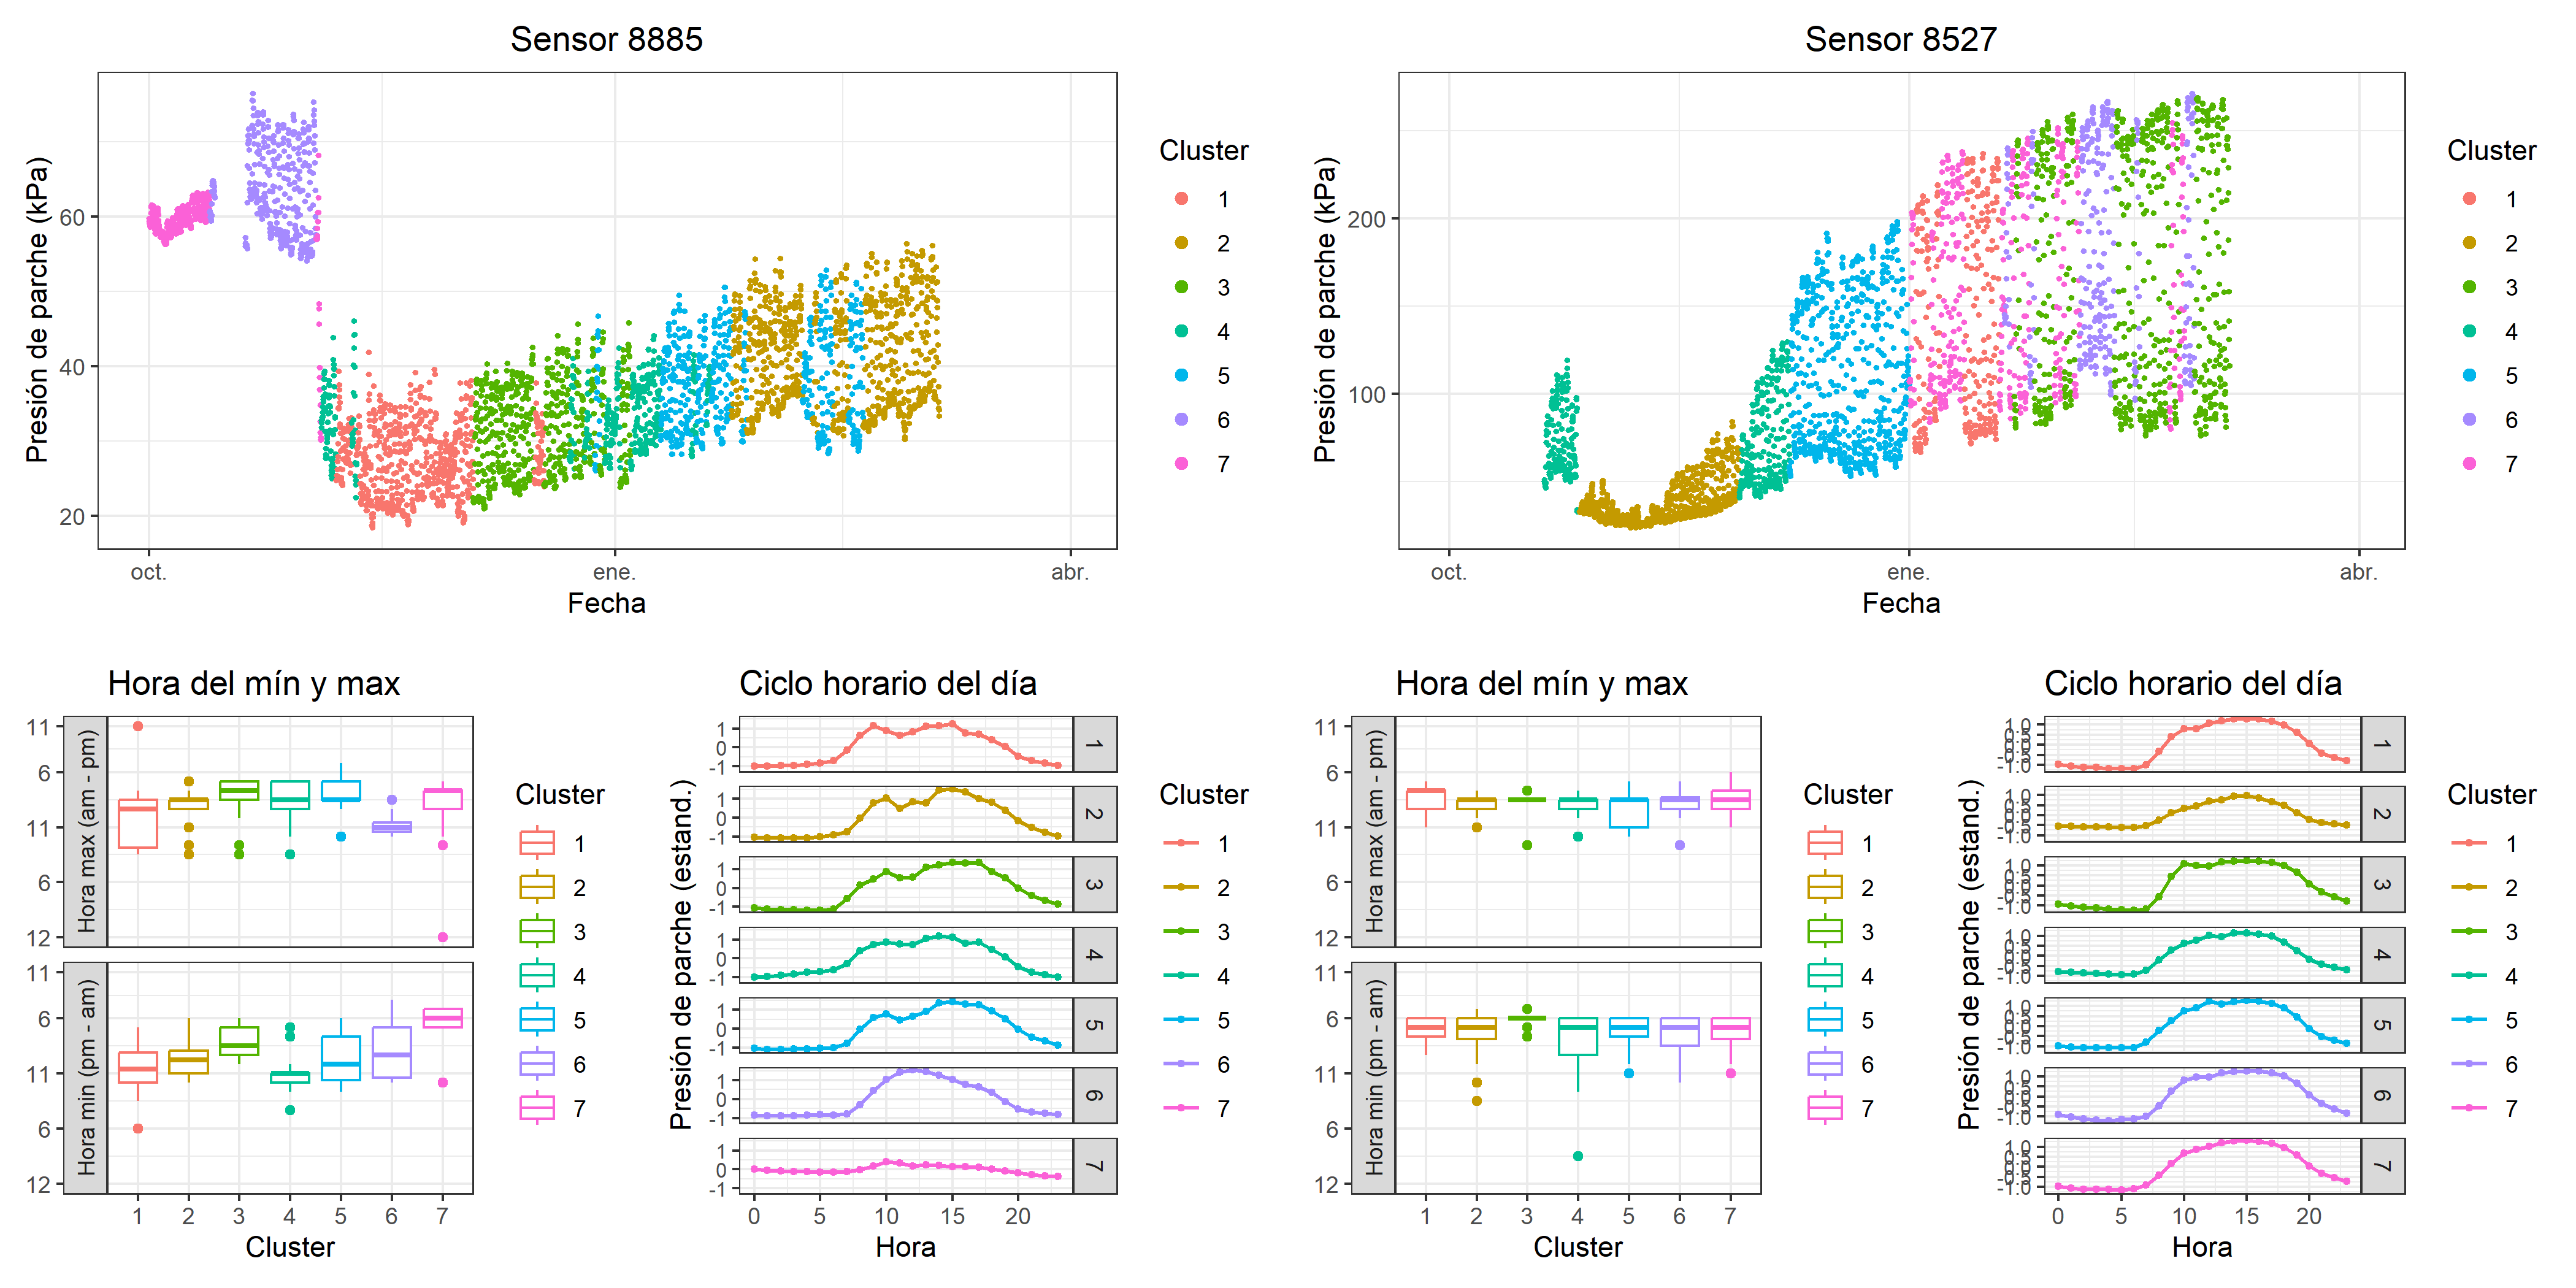
\includegraphics[keepaspectratio]{figuras/01_turgor_sensor/2022_2023_La_Esperanza_T3_Unidad_2.png}}

Unidad 3
\pandocbounded{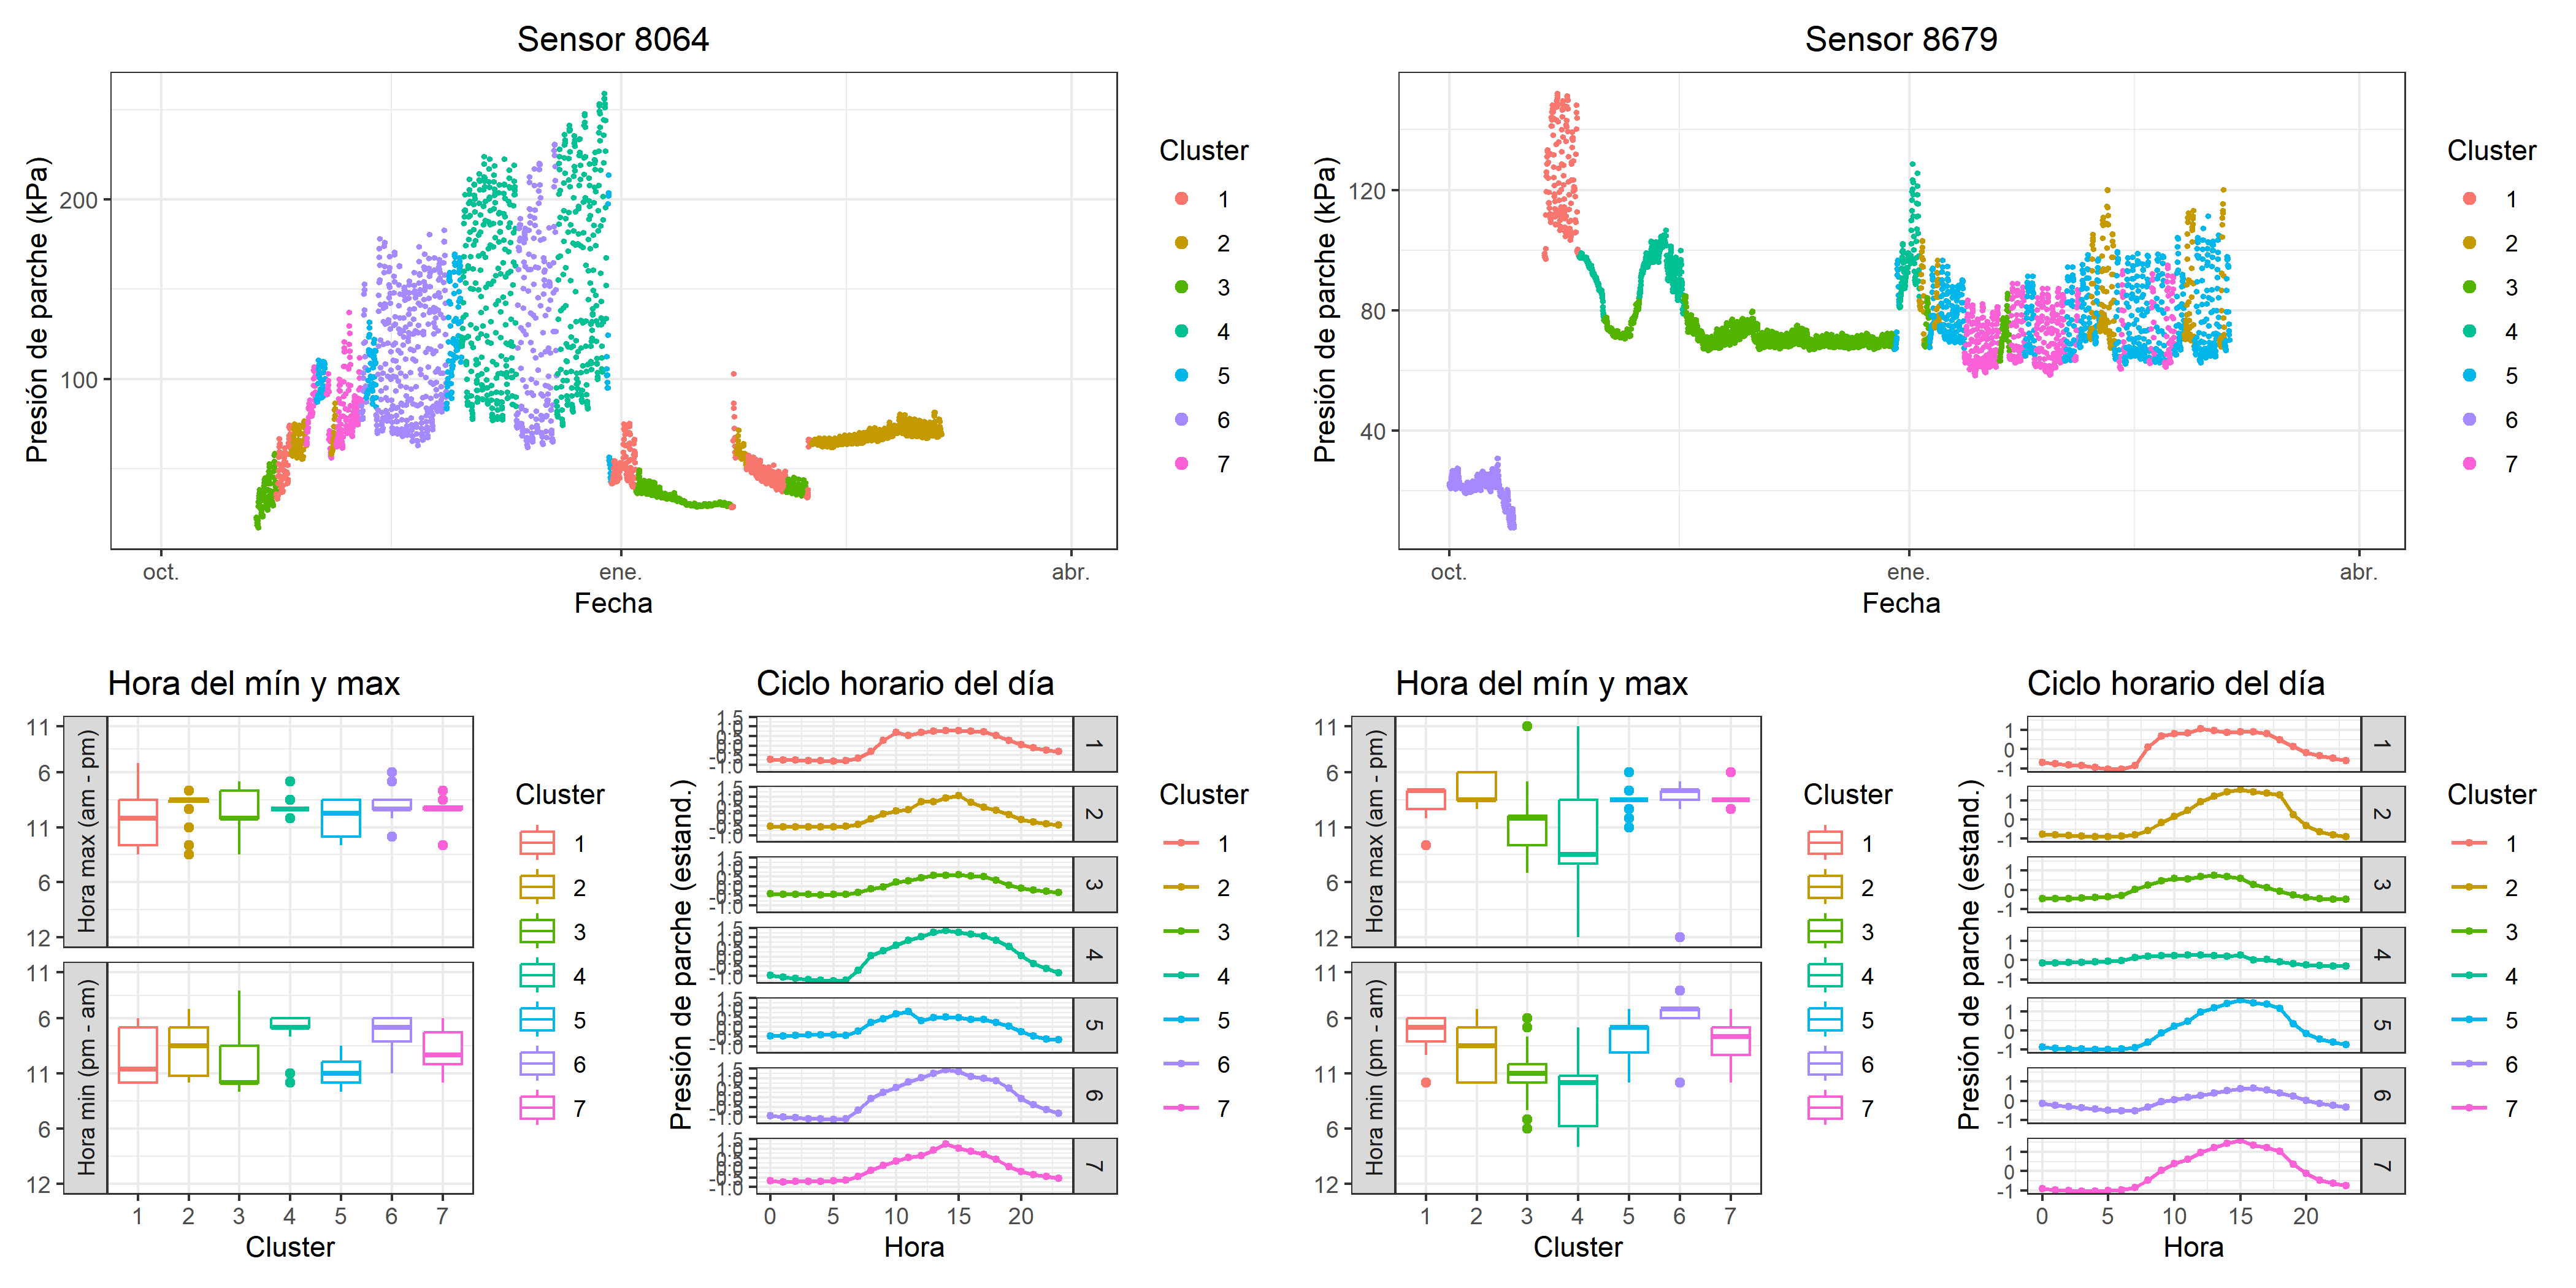
\includegraphics[keepaspectratio]{figuras/01_turgor_sensor/2022_2023_La_Esperanza_T3_Unidad_3.png}}

\chapter{T4 (2022-2023)}

Unidad 1
\pandocbounded{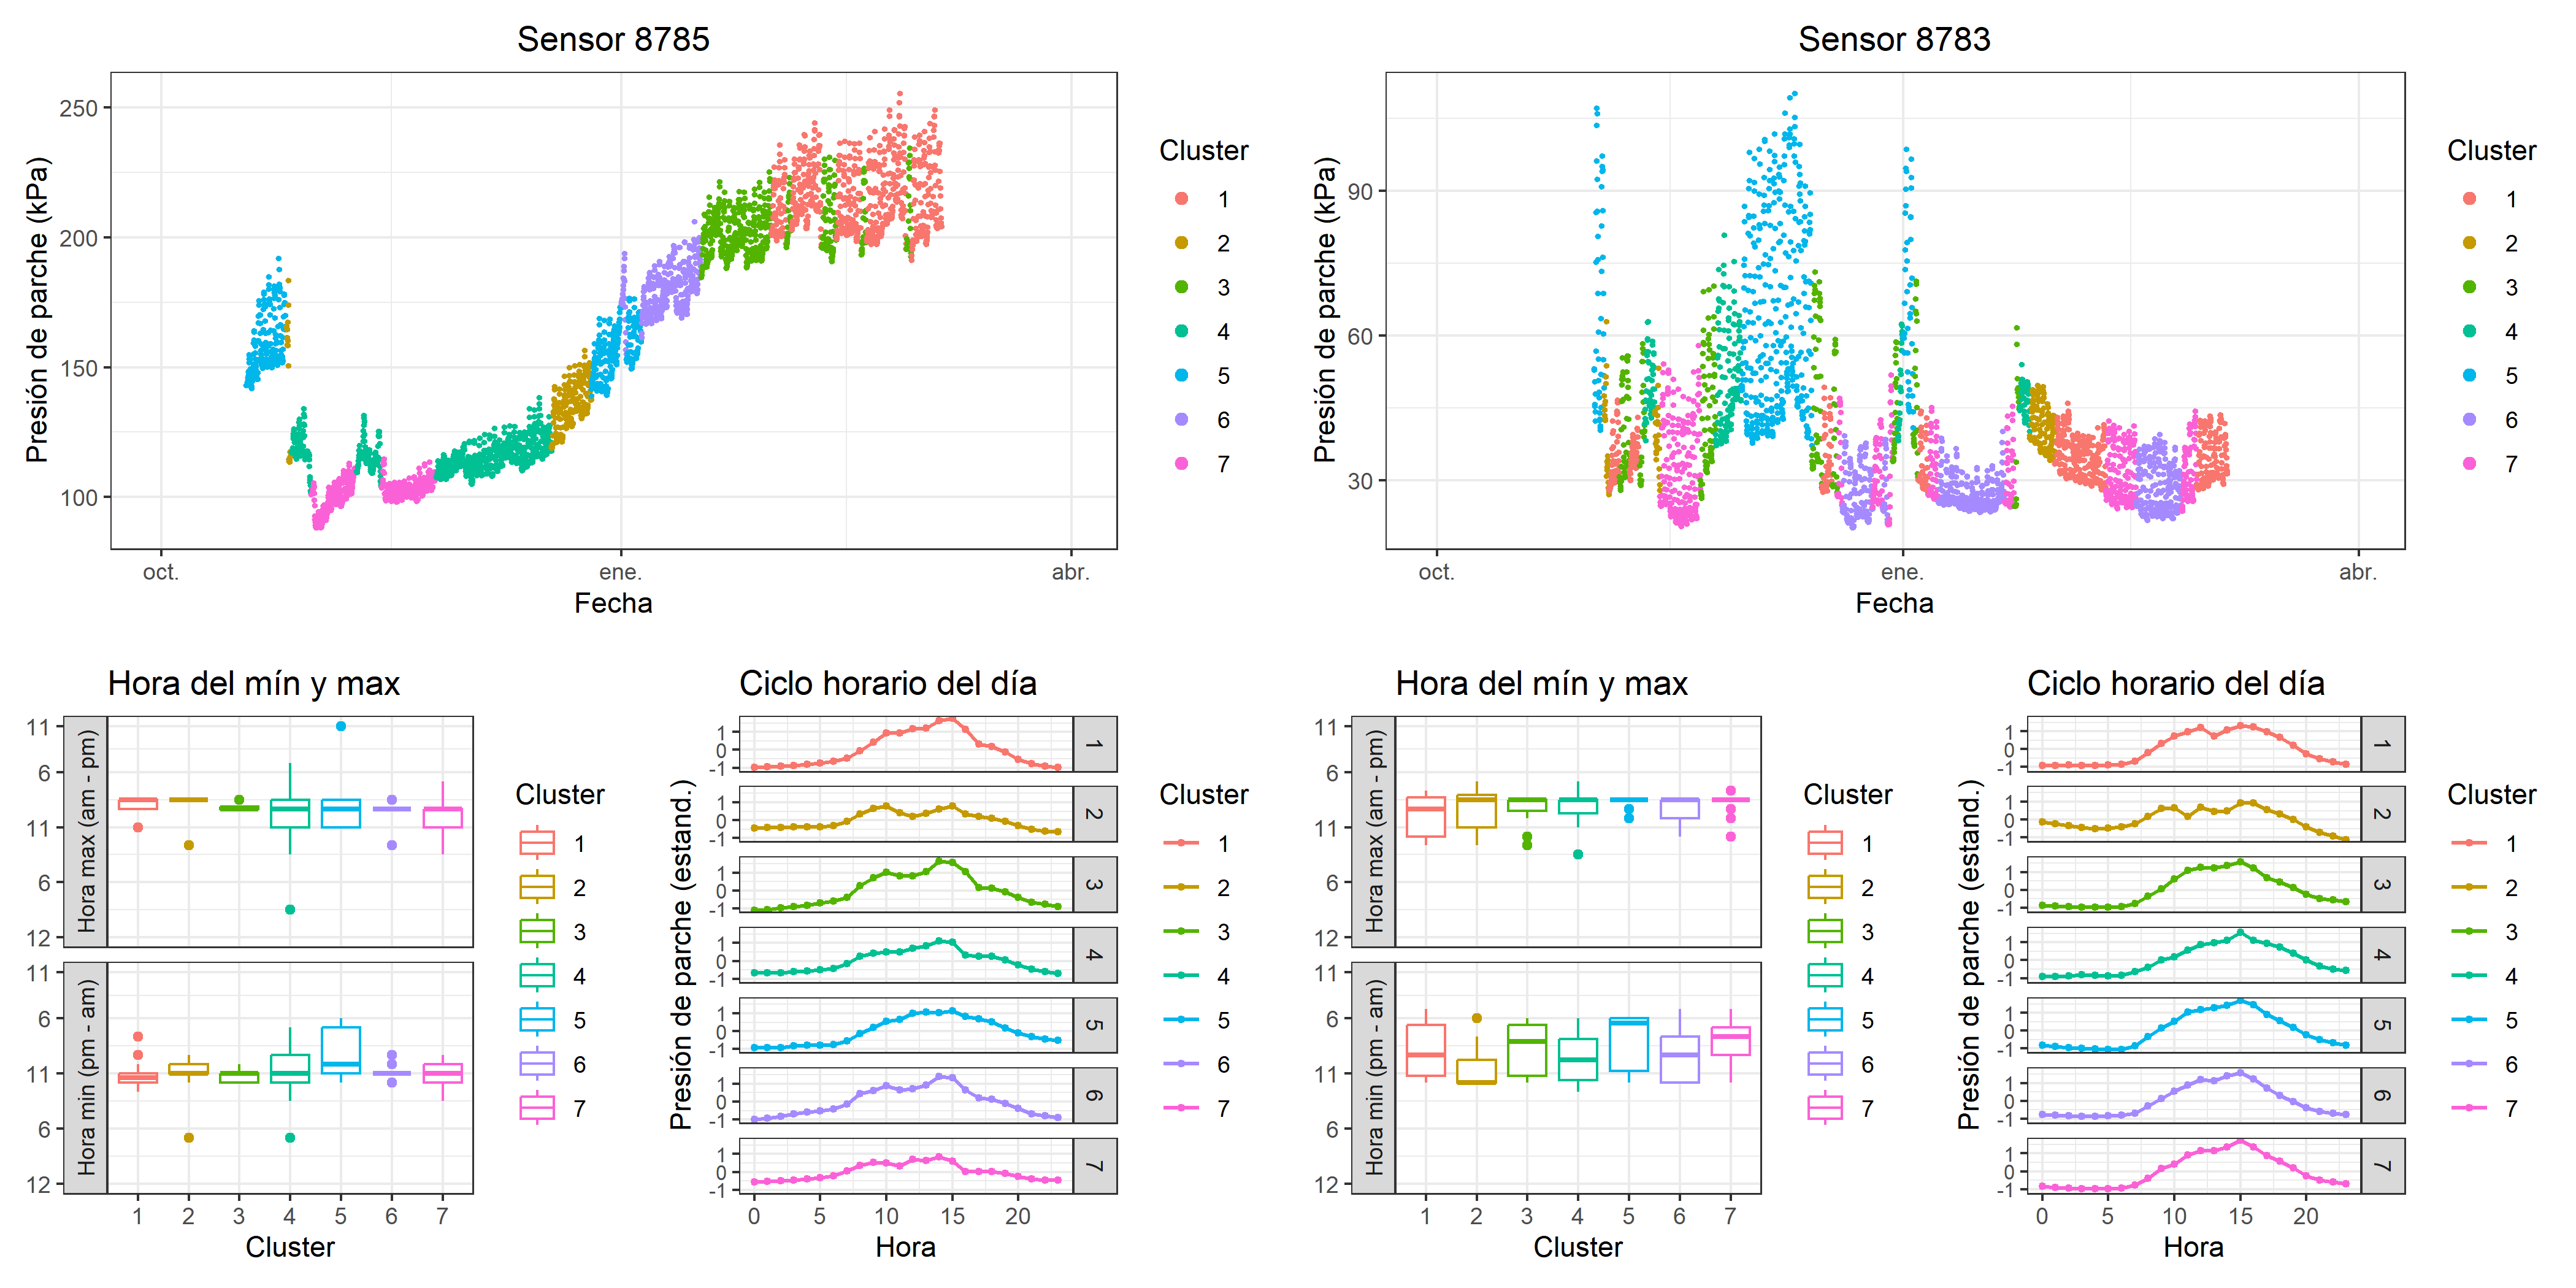
\includegraphics[keepaspectratio]{figuras/01_turgor_sensor/2022_2023_La_Esperanza_T4_Unidad_1.png}}

Unidad 2
\pandocbounded{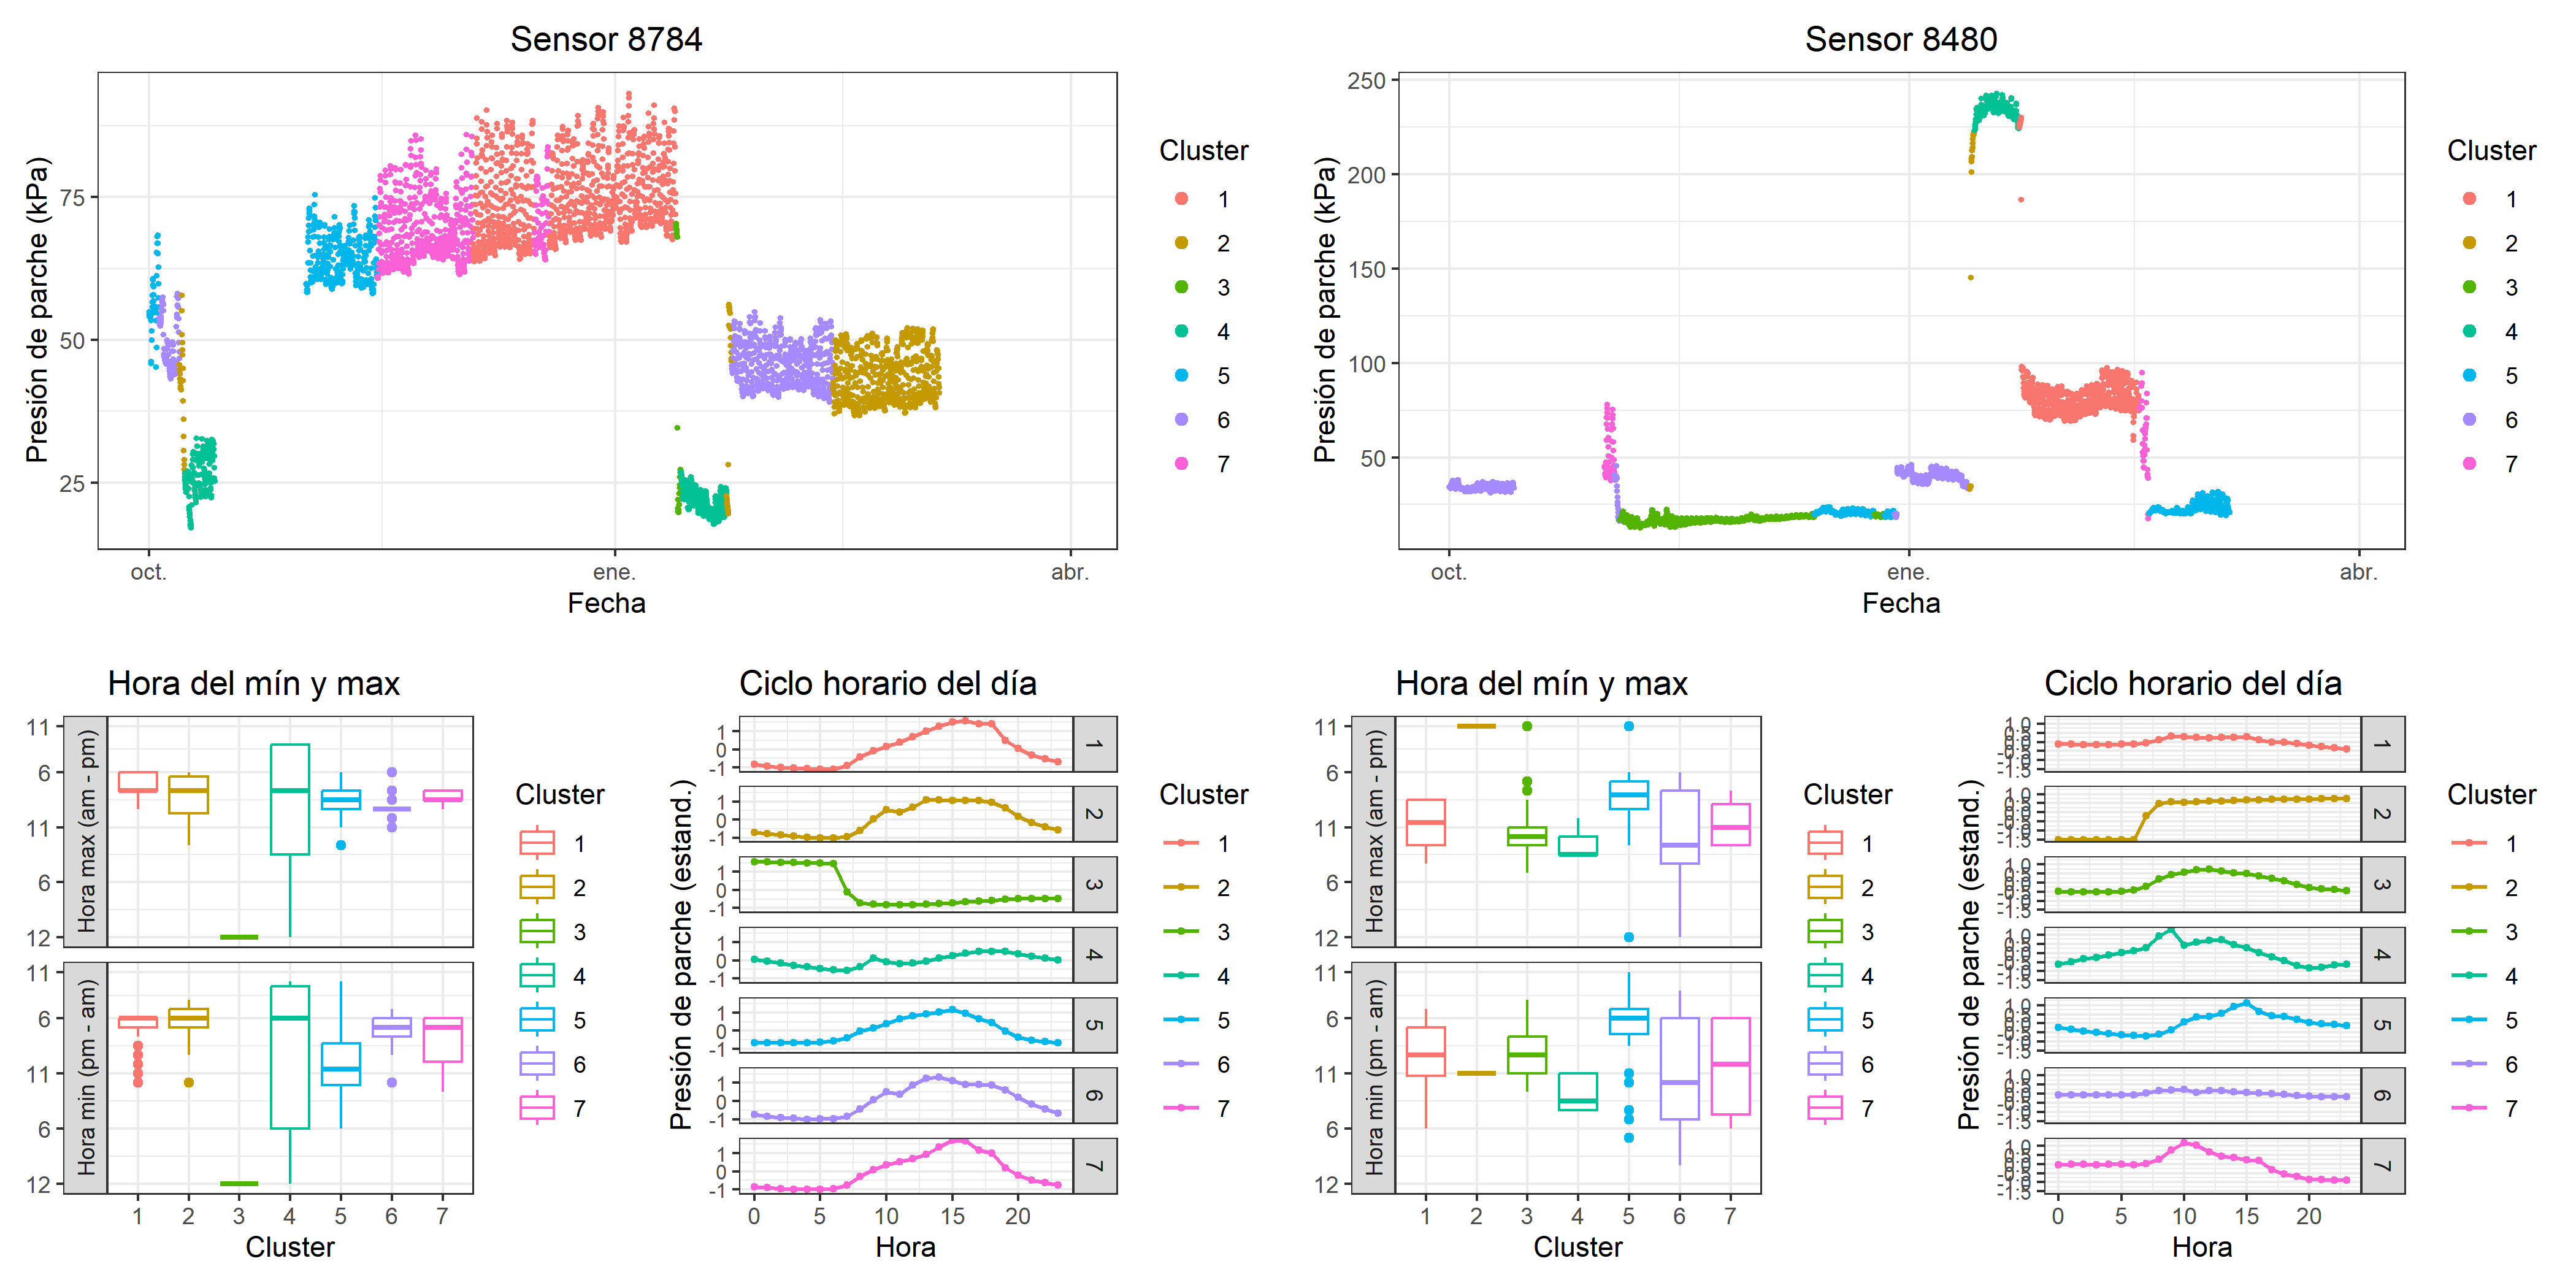
\includegraphics[keepaspectratio]{figuras/01_turgor_sensor/2022_2023_La_Esperanza_T4_Unidad_2.png}}

Unidad 3
\pandocbounded{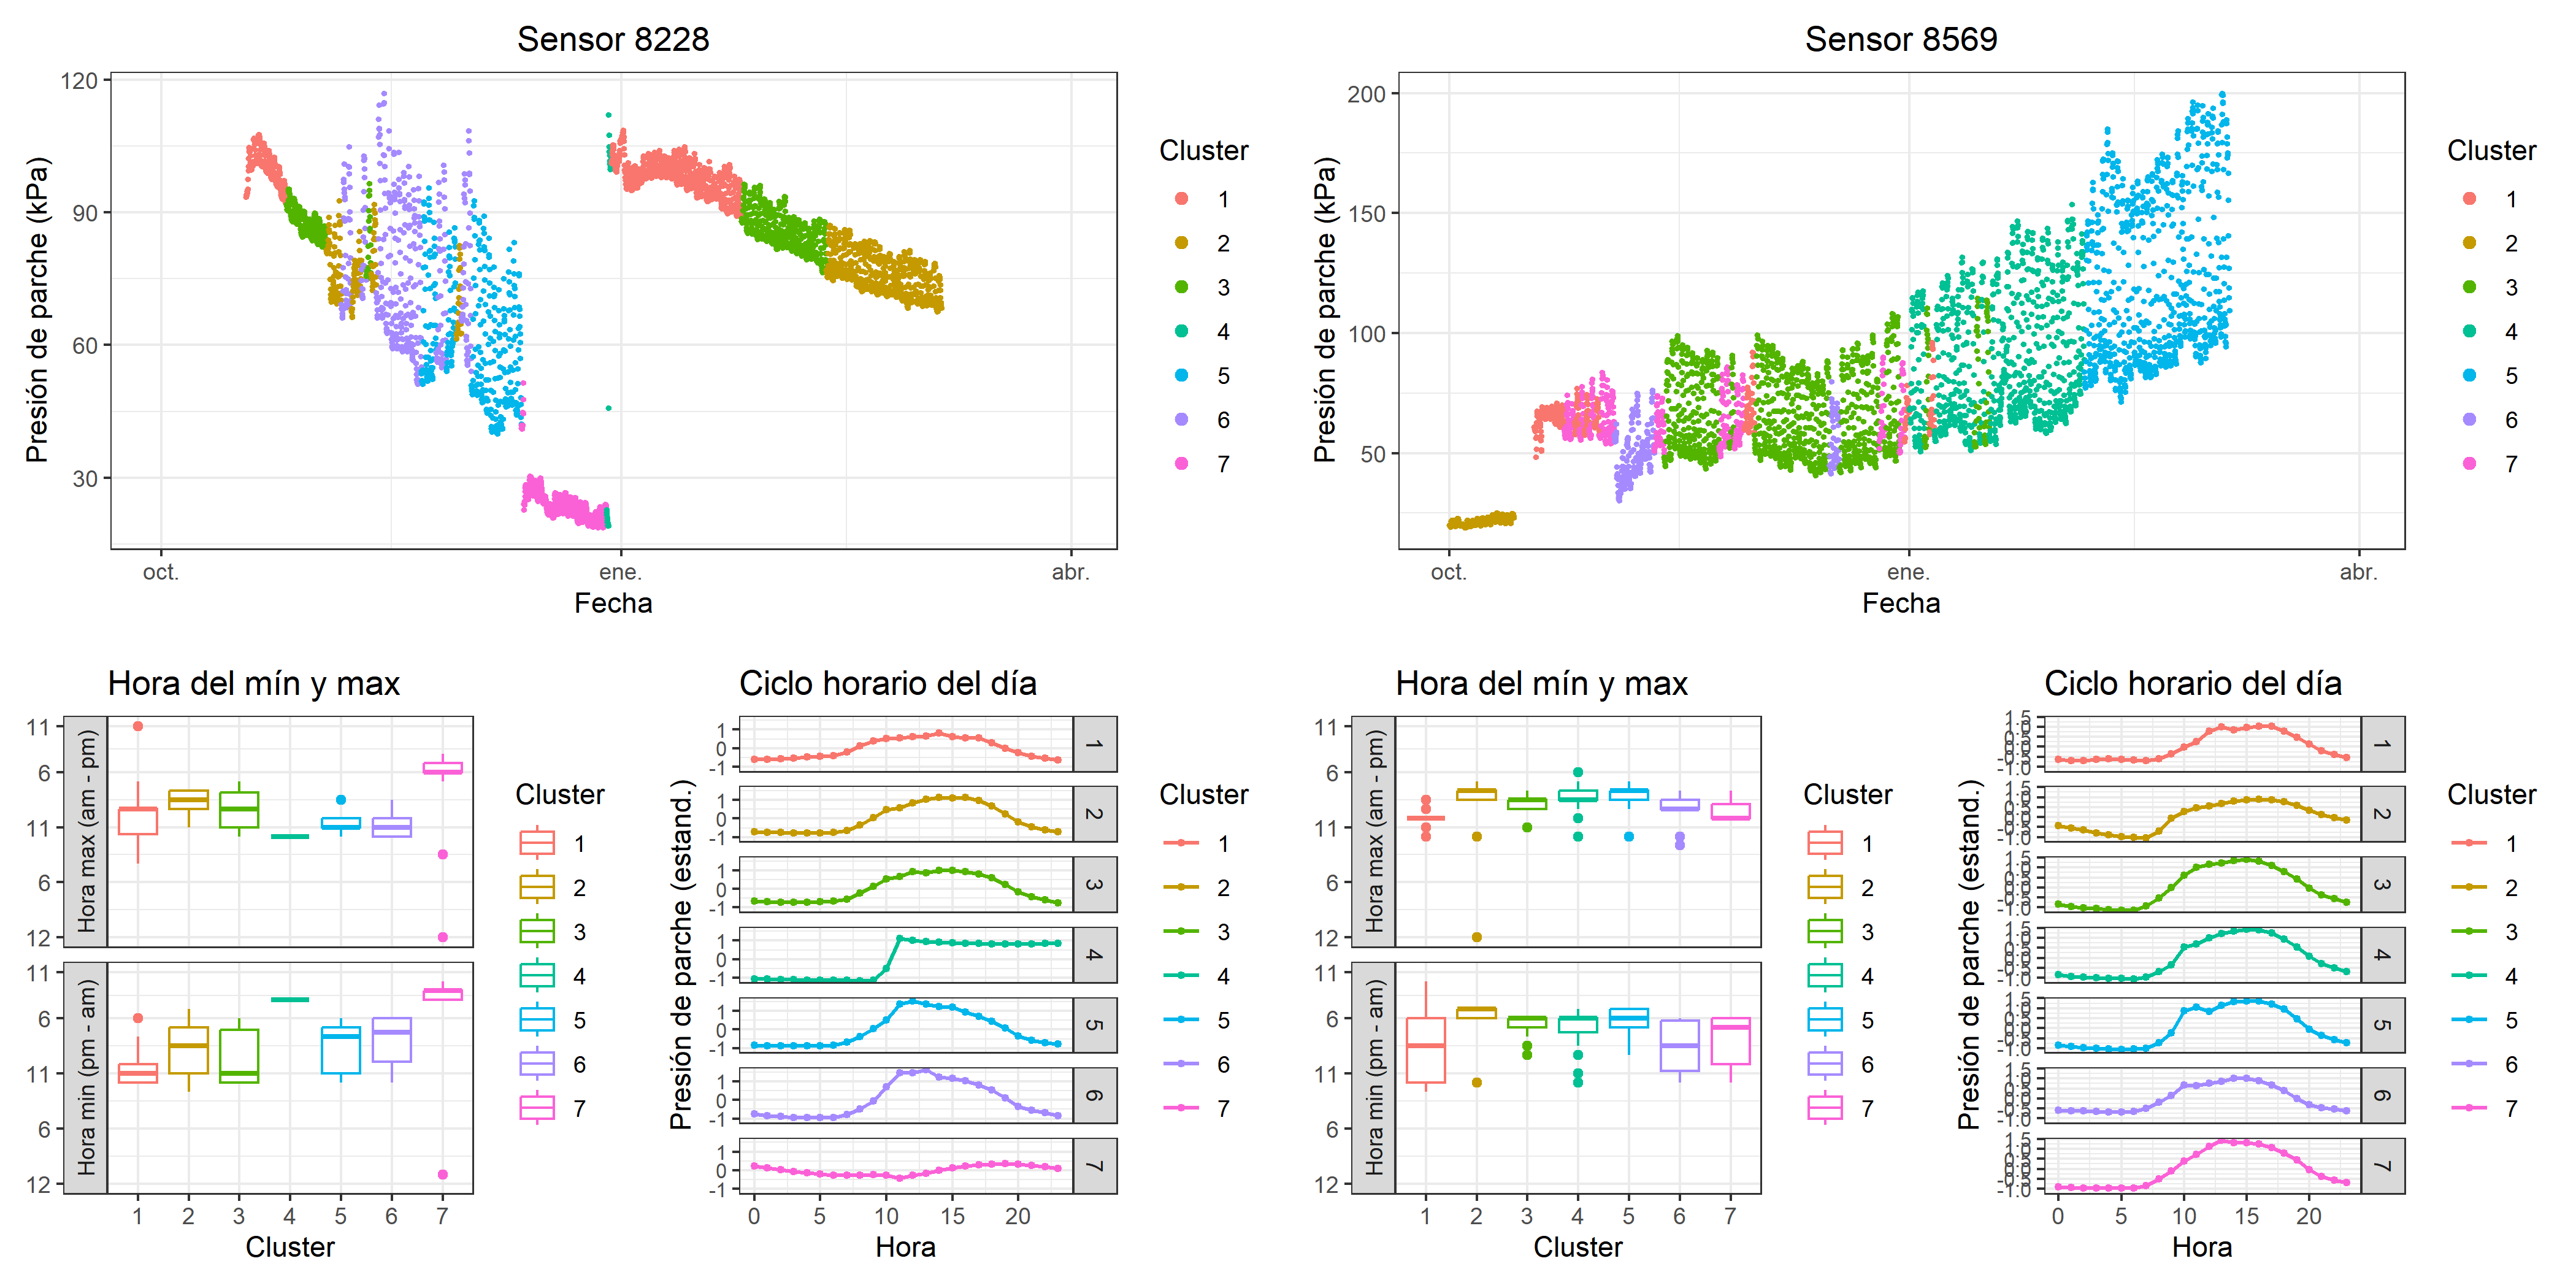
\includegraphics[keepaspectratio]{figuras/01_turgor_sensor/2022_2023_La_Esperanza_T4_Unidad_3.png}}

\chapter{T1 (2023-2024)}

Unidad 1
\pandocbounded{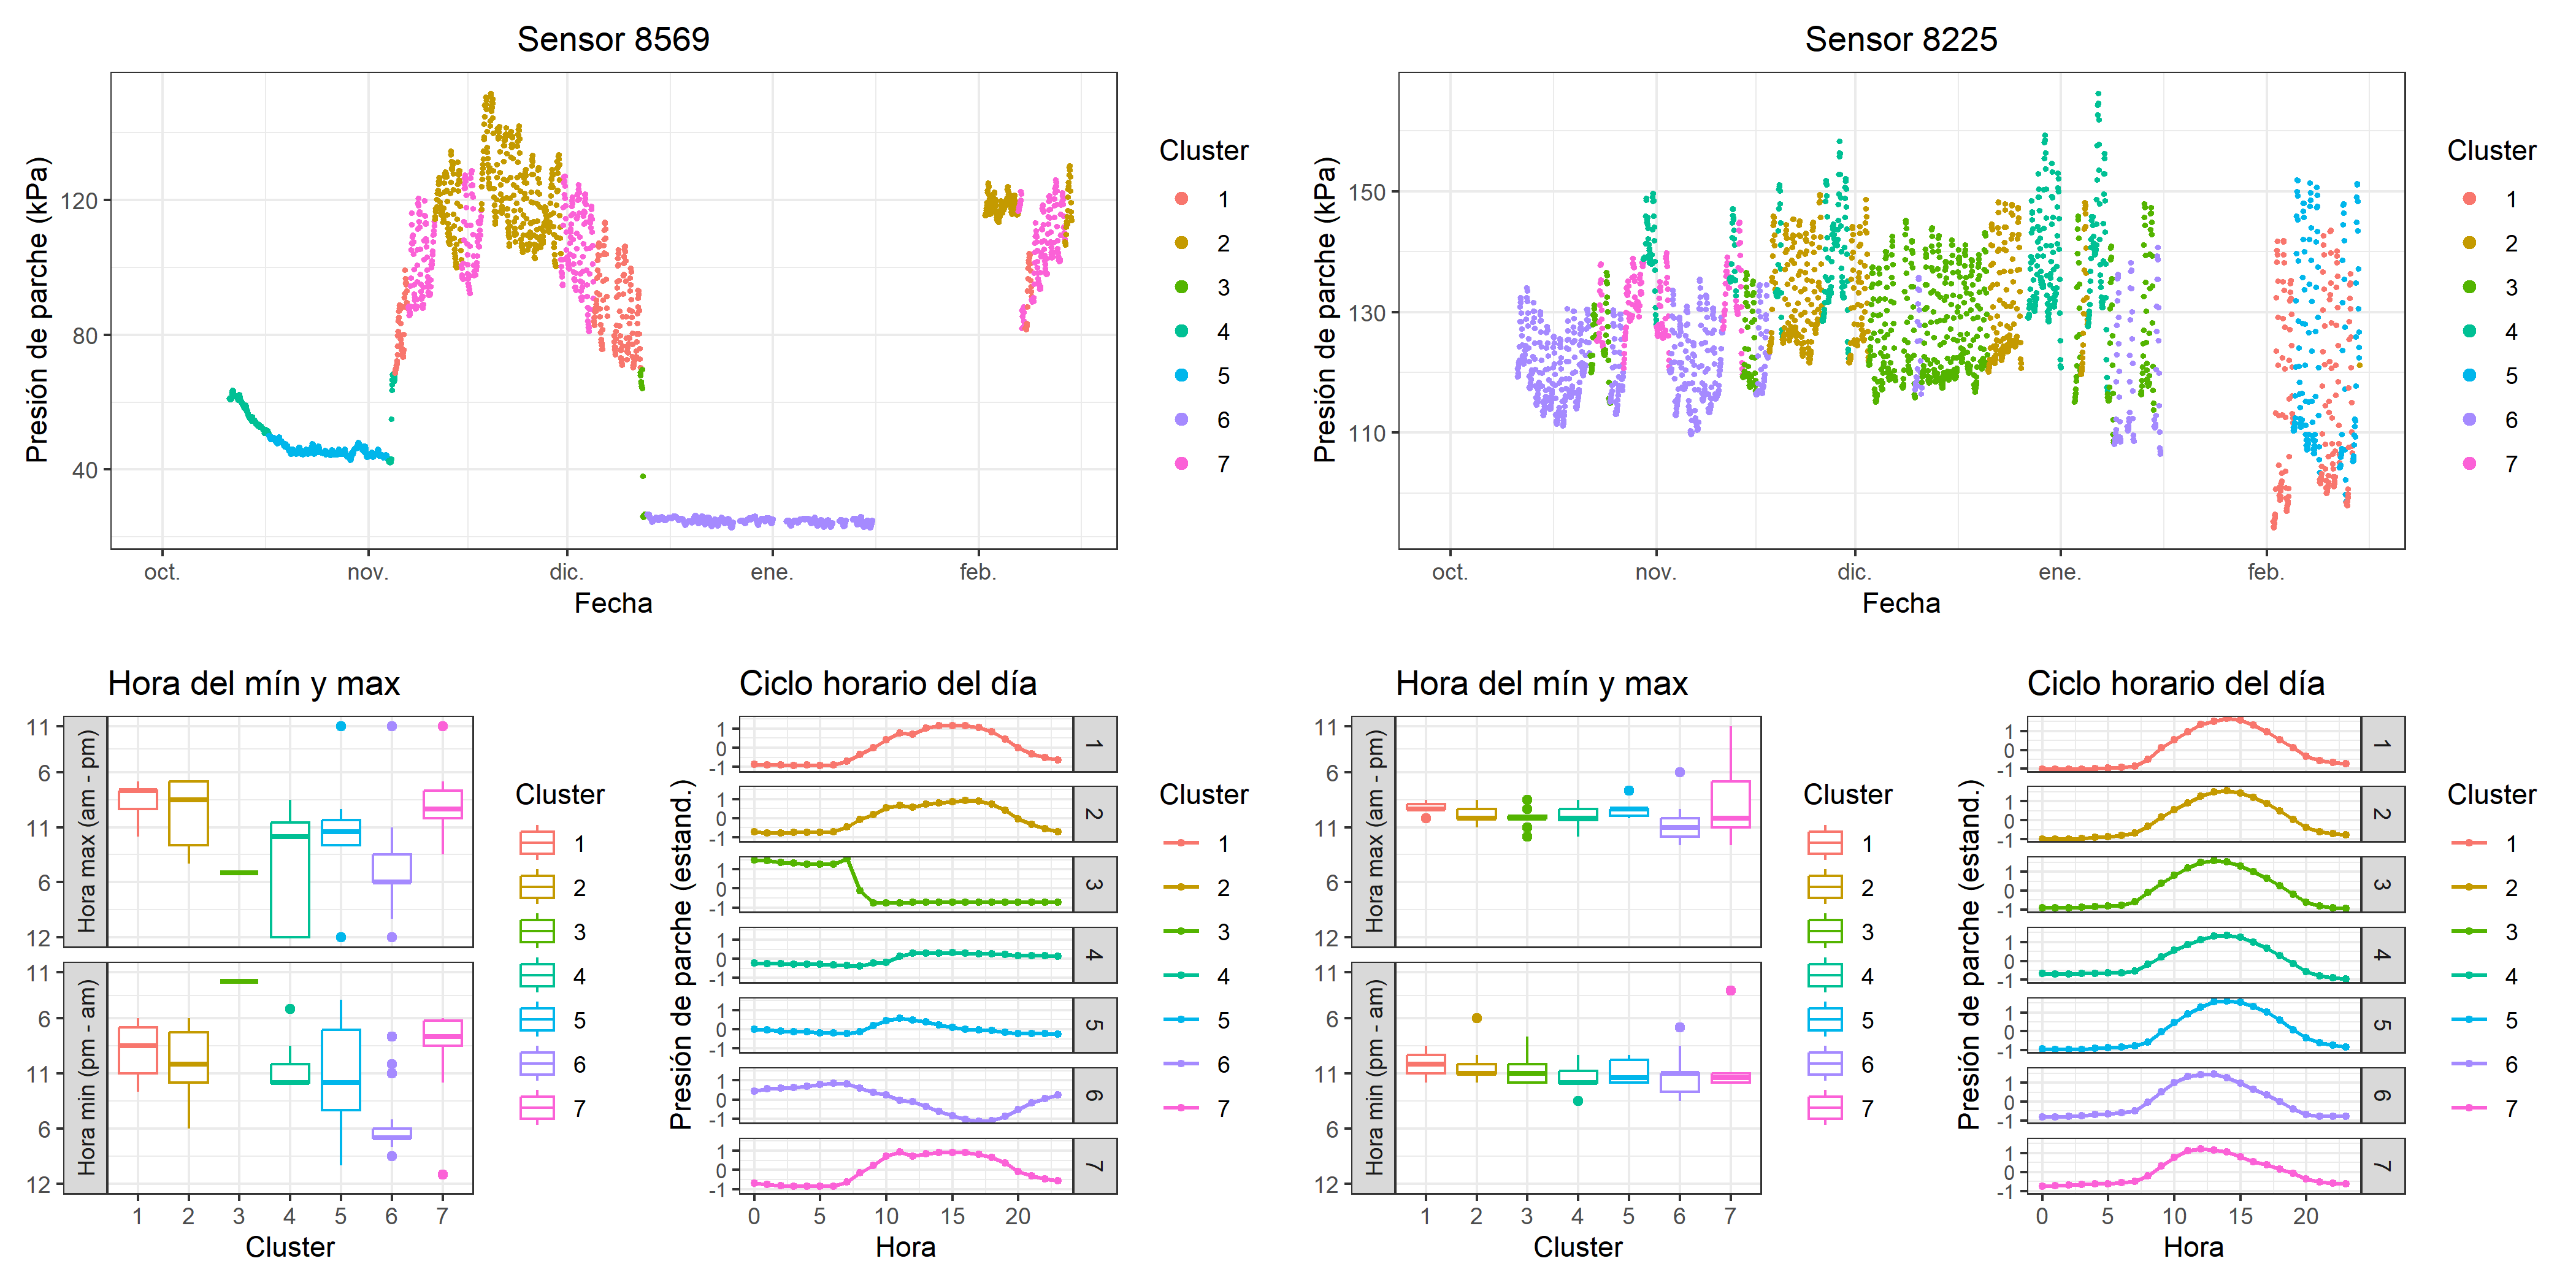
\includegraphics[keepaspectratio]{figuras/01_turgor_sensor/2023_2024_La_Esperanza_T1_Unidad_1.png}}

Unidad 2
\pandocbounded{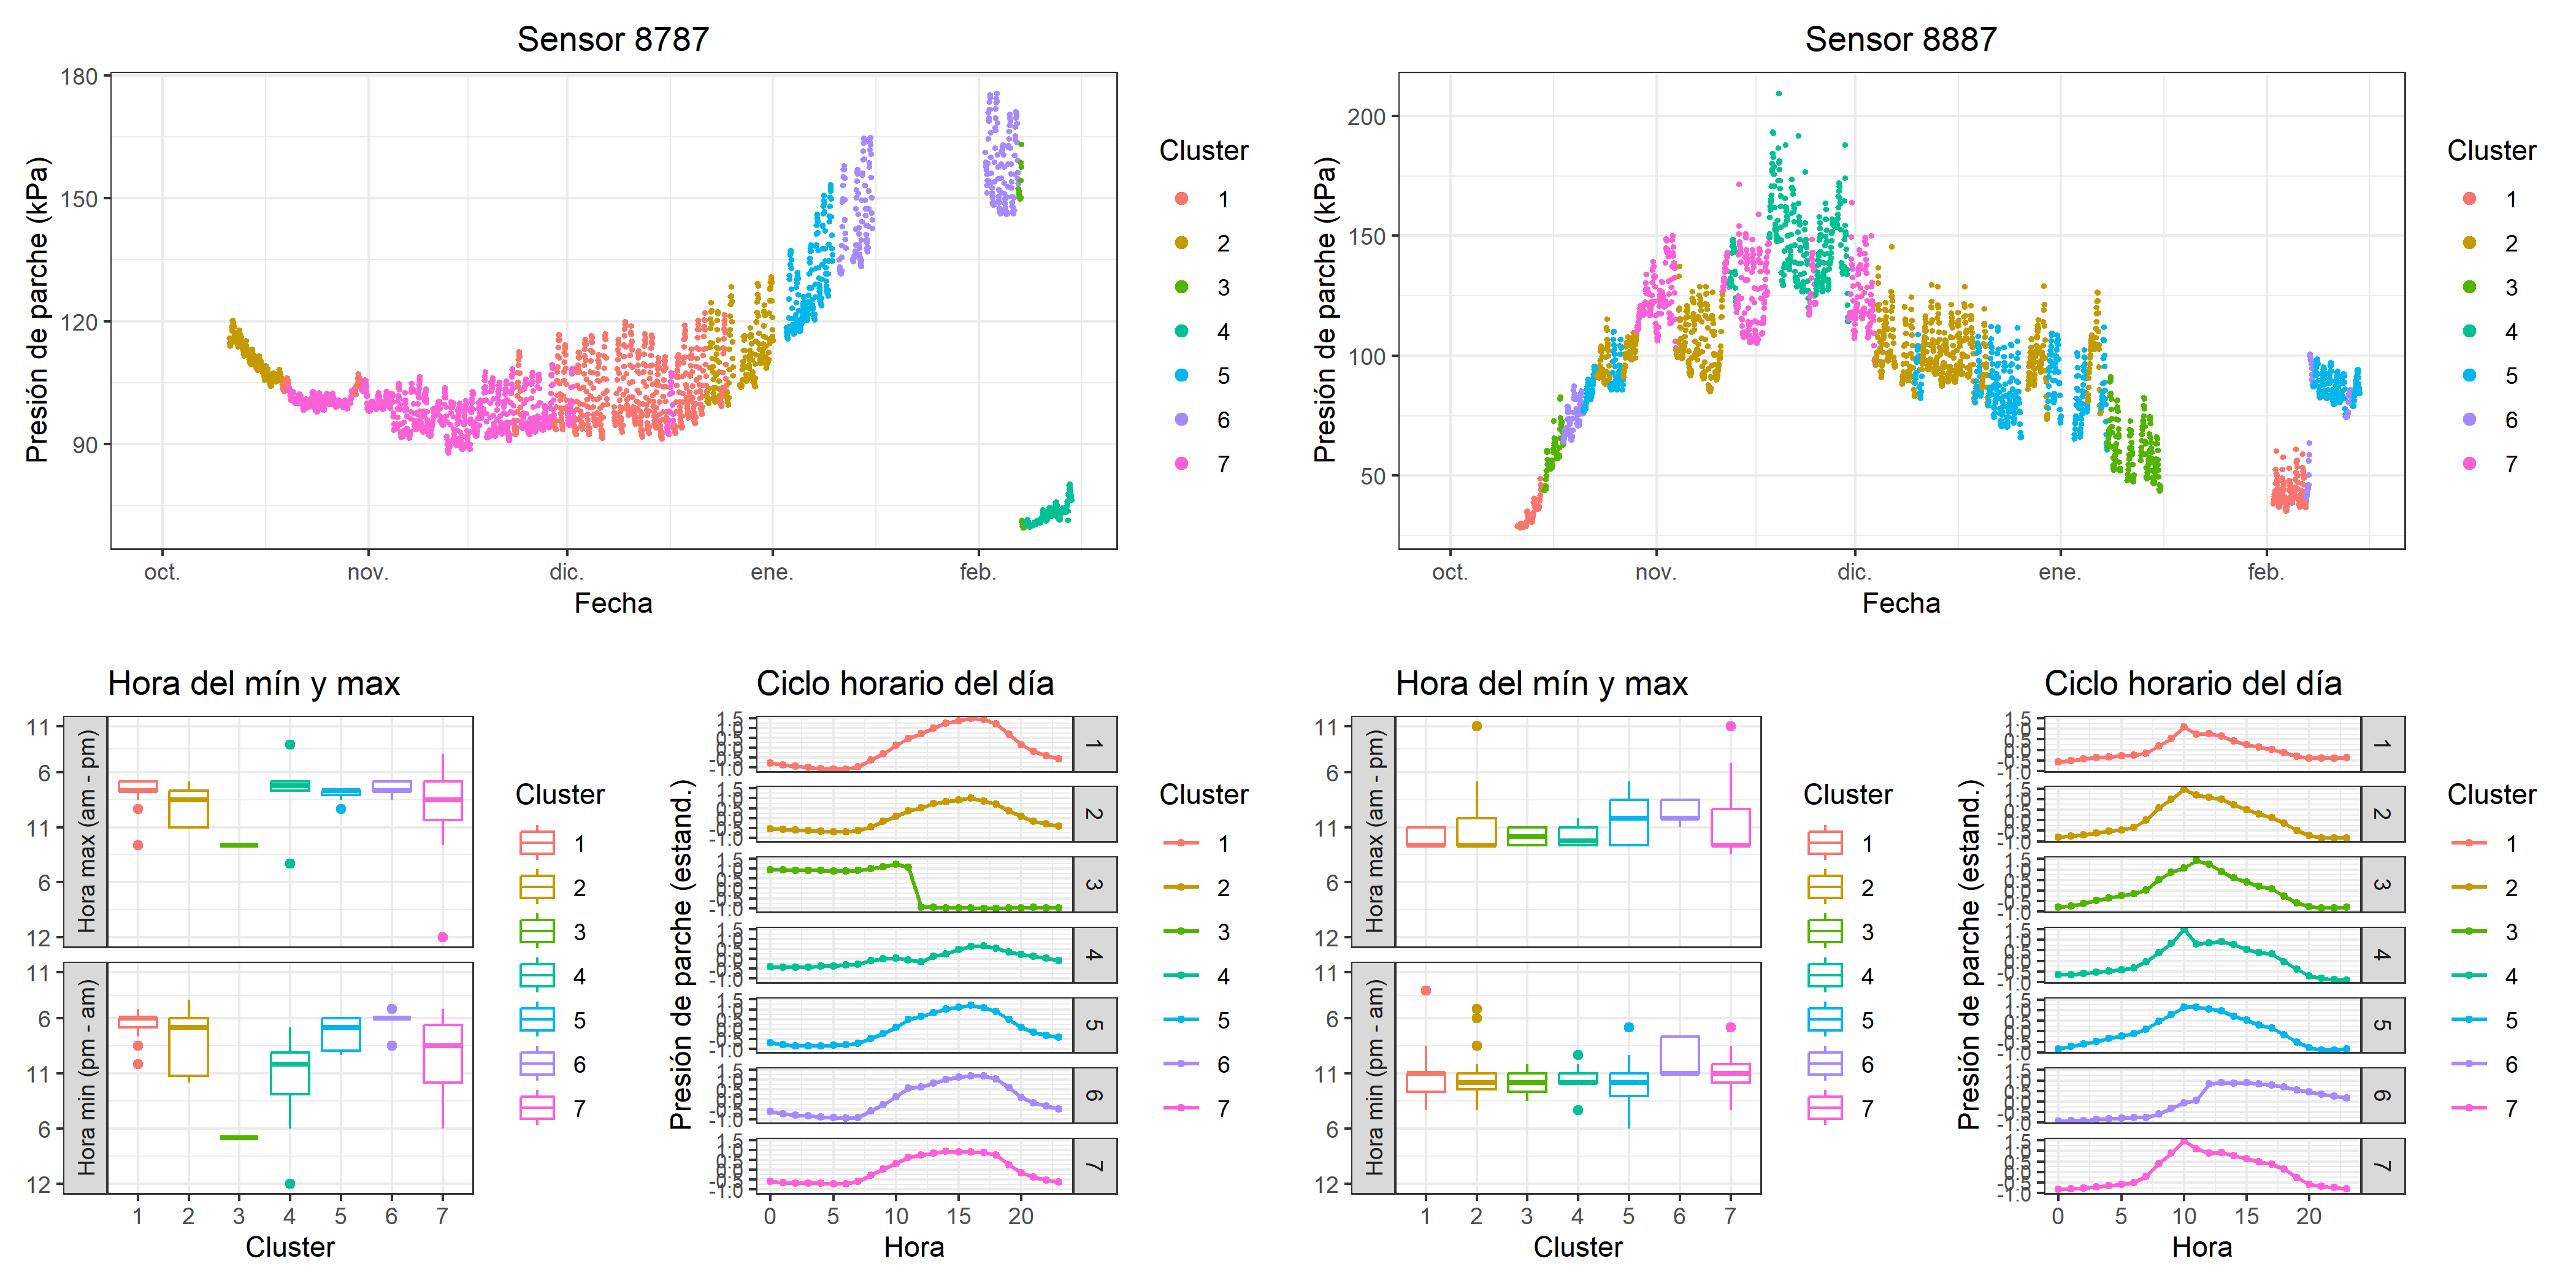
\includegraphics[keepaspectratio]{figuras/01_turgor_sensor/2023_2024_La_Esperanza_T1_Unidad_2.png}}

Unidad 3
\pandocbounded{\includegraphics[keepaspectratio]{figuras/01_turgor_sensor/2023_2024_La_Esperanza_T1_Unidad_3.png}}

\chapter{T2 (2023-2024)}

Unidad 1
\pandocbounded{\includegraphics[keepaspectratio]{figuras/01_turgor_sensor/2023_2024_La_Esperanza_T2_Unidad_1.png}}

Unidad 2
\pandocbounded{\includegraphics[keepaspectratio]{figuras/01_turgor_sensor/2023_2024_La_Esperanza_T2_Unidad_2.png}}

Unidad 3
\pandocbounded{\includegraphics[keepaspectratio]{figuras/01_turgor_sensor/2023_2024_La_Esperanza_T2_Unidad_3.png}}

\chapter{T3 (2023-2024)}

Unidad 1
\pandocbounded{\includegraphics[keepaspectratio]{figuras/01_turgor_sensor/2023_2024_La_Esperanza_T3_Unidad_1.png}}

Unidad 2
\pandocbounded{\includegraphics[keepaspectratio]{figuras/01_turgor_sensor/2023_2024_La_Esperanza_T3_Unidad_2.png}}

Unidad 3
\pandocbounded{\includegraphics[keepaspectratio]{figuras/01_turgor_sensor/2023_2024_La_Esperanza_T3_Unidad_3.png}}

\chapter{T4 (2023-2024)}

Unidad 1
\pandocbounded{\includegraphics[keepaspectratio]{figuras/01_turgor_sensor/2023_2024_La_Esperanza_T4_Unidad_1.png}}

Unidad 2
\pandocbounded{\includegraphics[keepaspectratio]{figuras/01_turgor_sensor/2023_2024_La_Esperanza_T4_Unidad_2.png}}

Unidad 3
\pandocbounded{\includegraphics[keepaspectratio]{figuras/01_turgor_sensor/2023_2024_La_Esperanza_T4_Unidad_3.png}}

\section{Rio Claro}\label{rio-claro}

\chapter{T1 (2022-2023)}

Unidad 1
\pandocbounded{\includegraphics[keepaspectratio]{figuras/01_turgor_sensor/2022_2023_Rio_Claro_T1_Unidad_1.png}}

Unidad 2
\pandocbounded{\includegraphics[keepaspectratio]{figuras/01_turgor_sensor/2022_2023_Rio_Claro_T1_Unidad_2.png}}

Unidad 3
\pandocbounded{\includegraphics[keepaspectratio]{figuras/01_turgor_sensor/2022_2023_Rio_Claro_T1_Unidad_3.png}}

\chapter{T2 (2022-2023)}

Unidad 1
\pandocbounded{\includegraphics[keepaspectratio]{figuras/01_turgor_sensor/2022_2023_Rio_Claro_T2_Unidad_1.png}}

Unidad 2
\pandocbounded{\includegraphics[keepaspectratio]{figuras/01_turgor_sensor/2022_2023_Rio_Claro_T2_Unidad_2.png}}

Unidad 3
\pandocbounded{\includegraphics[keepaspectratio]{figuras/01_turgor_sensor/2022_2023_Rio_Claro_T2_Unidad_3.png}}

\chapter{T3 (2022-2023)}

Unidad 1
\pandocbounded{\includegraphics[keepaspectratio]{figuras/01_turgor_sensor/2022_2023_Rio_Claro_T3_Unidad_1.png}}

Unidad 2
\pandocbounded{\includegraphics[keepaspectratio]{figuras/01_turgor_sensor/2022_2023_Rio_Claro_T3_Unidad_2.png}}

Unidad 3
\pandocbounded{\includegraphics[keepaspectratio]{figuras/01_turgor_sensor/2022_2023_Rio_Claro_T3_Unidad_3.png}}

\chapter{T4 (2022-2023)}

Unidad 1
\pandocbounded{\includegraphics[keepaspectratio]{figuras/01_turgor_sensor/2022_2023_Rio_Claro_T4_Unidad_1.png}}

Unidad 2
\pandocbounded{\includegraphics[keepaspectratio]{figuras/01_turgor_sensor/2022_2023_Rio_Claro_T4_Unidad_2.png}}

Unidad 3
\pandocbounded{\includegraphics[keepaspectratio]{figuras/01_turgor_sensor/2022_2023_Rio_Claro_T4_Unidad_3.png}}

\chapter{T1 (2023-2024)}

Unidad 1
\pandocbounded{\includegraphics[keepaspectratio]{figuras/01_turgor_sensor/2023_2024_Rio_Claro_T1_Unidad_1.png}}

Unidad 2
\pandocbounded{\includegraphics[keepaspectratio]{figuras/01_turgor_sensor/2023_2024_Rio_Claro_T1_Unidad_2.png}}

Unidad 3
\pandocbounded{\includegraphics[keepaspectratio]{figuras/01_turgor_sensor/2023_2024_Rio_Claro_T1_Unidad_3.png}}

\chapter{T2 (2023-2024)}

Unidad 1
\pandocbounded{\includegraphics[keepaspectratio]{figuras/01_turgor_sensor/2023_2024_Rio_Claro_T2_Unidad_1.png}}

Unidad 2
\pandocbounded{\includegraphics[keepaspectratio]{figuras/01_turgor_sensor/2023_2024_Rio_Claro_T2_Unidad_2.png}}

Unidad 3
\pandocbounded{\includegraphics[keepaspectratio]{figuras/01_turgor_sensor/2023_2024_Rio_Claro_T2_Unidad_3.png}}

\chapter{T3 (2023-2024)}

Unidad 1
\pandocbounded{\includegraphics[keepaspectratio]{figuras/01_turgor_sensor/2023_2024_Rio_Claro_T3_Unidad_1.png}}

Unidad 2
\pandocbounded{\includegraphics[keepaspectratio]{figuras/01_turgor_sensor/2023_2024_Rio_Claro_T3_Unidad_2.png}}

Unidad 3
\pandocbounded{\includegraphics[keepaspectratio]{figuras/01_turgor_sensor/2023_2024_Rio_Claro_T3_Unidad_3.png}}

\chapter{T4 (2023-2024)}

Unidad 1
\pandocbounded{\includegraphics[keepaspectratio]{figuras/01_turgor_sensor/2023_2024_Rio_Claro_T4_Unidad_1.png}}

Unidad 2
\pandocbounded{\includegraphics[keepaspectratio]{figuras/01_turgor_sensor/2023_2024_Rio_Claro_T4_Unidad_2.png}}

Unidad 3
\pandocbounded{\includegraphics[keepaspectratio]{figuras/01_turgor_sensor/2023_2024_Rio_Claro_T4_Unidad_3.png}}

\chapter{Limpieza de datos: eliminación de
clusters}\label{limpieza-de-datos-eliminaciuxf3n-de-clusters}

Para limpiar los datos de turgor, se emplearon series temporales de VPD
y temperatura provenientes de las estaciones meteorológicas de los dos
sitios de estudio. Se procedió a calcular el coeficiente de correlación
entre cada cluster y los valores de VPD y temperatura respecto al tiempo
(escala horaria) y el sitio. Se obtuvo un coeficiente de correlación
promedio en relación con ambas variables, y se estableció un umbral de
corte de r \textgreater{} 0.5. Aquellos clusters de turgor cuyo promedio
de correlación resultó menor a 0.5 fueron descartados.

\section{La Esperanza}\label{la-esperanza-1}

\chapter{T1 (2022-2023)}

Unidad 1
\pandocbounded{\includegraphics[keepaspectratio]{figuras/02_turgor_limpiado/2022_2023_La_Esperanza_T1_Unidad_1.png}}

Unidad 2
\pandocbounded{\includegraphics[keepaspectratio]{figuras/02_turgor_limpiado/2022_2023_La_Esperanza_T1_Unidad_2.png}}

Unidad 3
\pandocbounded{\includegraphics[keepaspectratio]{figuras/02_turgor_limpiado/2022_2023_La_Esperanza_T1_Unidad_3.png}}

\chapter{T2 (2022-2023)}

Unidad 1
\pandocbounded{\includegraphics[keepaspectratio]{figuras/02_turgor_limpiado/2022_2023_La_Esperanza_T2_Unidad_1.png}}

Unidad 2
\pandocbounded{\includegraphics[keepaspectratio]{figuras/02_turgor_limpiado/2022_2023_La_Esperanza_T2_Unidad_2.png}}

Unidad 3
\pandocbounded{\includegraphics[keepaspectratio]{figuras/02_turgor_limpiado/2022_2023_La_Esperanza_T2_Unidad_3.png}}

\chapter{T3 (2022-2023)}

Unidad 1
\pandocbounded{\includegraphics[keepaspectratio]{figuras/02_turgor_limpiado/2022_2023_La_Esperanza_T3_Unidad_1.png}}

Unidad 2
\pandocbounded{\includegraphics[keepaspectratio]{figuras/02_turgor_limpiado/2022_2023_La_Esperanza_T3_Unidad_2.png}}

Unidad 3
\pandocbounded{\includegraphics[keepaspectratio]{figuras/02_turgor_limpiado/2022_2023_La_Esperanza_T3_Unidad_3.png}}

\chapter{T4 (2022-2023)}

Unidad 1
\pandocbounded{\includegraphics[keepaspectratio]{figuras/02_turgor_limpiado/2022_2023_La_Esperanza_T4_Unidad_1.png}}

Unidad 2
\pandocbounded{\includegraphics[keepaspectratio]{figuras/02_turgor_limpiado/2022_2023_La_Esperanza_T4_Unidad_2.png}}

Unidad 3
\pandocbounded{\includegraphics[keepaspectratio]{figuras/02_turgor_limpiado/2022_2023_La_Esperanza_T4_Unidad_3.png}}

\chapter{T1 (2023-2024)}

Unidad 1
\pandocbounded{\includegraphics[keepaspectratio]{figuras/02_turgor_limpiado/2023_2024_La_Esperanza_T1_Unidad_1.png}}

Unidad 2
\pandocbounded{\includegraphics[keepaspectratio]{figuras/02_turgor_limpiado/2023_2024_La_Esperanza_T1_Unidad_2.png}}

Unidad 3
\pandocbounded{\includegraphics[keepaspectratio]{figuras/02_turgor_limpiado/2023_2024_La_Esperanza_T1_Unidad_3.png}}

\chapter{T2 (2023-2024)}

Unidad 1
\pandocbounded{\includegraphics[keepaspectratio]{figuras/02_turgor_limpiado/2023_2024_La_Esperanza_T2_Unidad_1.png}}

Unidad 2
\pandocbounded{\includegraphics[keepaspectratio]{figuras/02_turgor_limpiado/2023_2024_La_Esperanza_T2_Unidad_2.png}}

Unidad 3
\pandocbounded{\includegraphics[keepaspectratio]{figuras/02_turgor_limpiado/2023_2024_La_Esperanza_T2_Unidad_3.png}}

\chapter{T3 (2023-2024)}

Unidad 1
\pandocbounded{\includegraphics[keepaspectratio]{figuras/02_turgor_limpiado/2023_2024_La_Esperanza_T3_Unidad_1.png}}

Unidad 2
\pandocbounded{\includegraphics[keepaspectratio]{figuras/02_turgor_limpiado/2023_2024_La_Esperanza_T3_Unidad_2.png}}

Unidad 3
\pandocbounded{\includegraphics[keepaspectratio]{figuras/02_turgor_limpiado/2023_2024_La_Esperanza_T3_Unidad_3.png}}

\chapter{T4 (2023-2024)}

Unidad 1
\pandocbounded{\includegraphics[keepaspectratio]{figuras/02_turgor_limpiado/2023_2024_La_Esperanza_T4_Unidad_1.png}}

Unidad 2
\pandocbounded{\includegraphics[keepaspectratio]{figuras/02_turgor_limpiado/2023_2024_La_Esperanza_T4_Unidad_2.png}}

Unidad 3
\pandocbounded{\includegraphics[keepaspectratio]{figuras/02_turgor_limpiado/2023_2024_La_Esperanza_T4_Unidad_3.png}}

\section{Rio Claro}\label{rio-claro-1}

\chapter{T1 (2022-2023)}

Unidad 1
\pandocbounded{\includegraphics[keepaspectratio]{figuras/02_turgor_limpiado/2022_2023_Rio_Claro_T1_Unidad_1.png}}

Unidad 2
\pandocbounded{\includegraphics[keepaspectratio]{figuras/02_turgor_limpiado/2022_2023_Rio_Claro_T1_Unidad_2.png}}

Unidad 3
\pandocbounded{\includegraphics[keepaspectratio]{figuras/02_turgor_limpiado/2022_2023_Rio_Claro_T1_Unidad_3.png}}

\chapter{T2 (2022-2023)}

Unidad 1
\pandocbounded{\includegraphics[keepaspectratio]{figuras/02_turgor_limpiado/2022_2023_Rio_Claro_T2_Unidad_1.png}}

Unidad 2
\pandocbounded{\includegraphics[keepaspectratio]{figuras/02_turgor_limpiado/2022_2023_Rio_Claro_T2_Unidad_2.png}}

Unidad 3
\pandocbounded{\includegraphics[keepaspectratio]{figuras/02_turgor_limpiado/2022_2023_Rio_Claro_T2_Unidad_3.png}}

\chapter{T3 (2022-2023)}

Unidad 1
\pandocbounded{\includegraphics[keepaspectratio]{figuras/02_turgor_limpiado/2022_2023_Rio_Claro_T3_Unidad_1.png}}

Unidad 2
\pandocbounded{\includegraphics[keepaspectratio]{figuras/02_turgor_limpiado/2022_2023_Rio_Claro_T3_Unidad_2.png}}

Unidad 3
\pandocbounded{\includegraphics[keepaspectratio]{figuras/02_turgor_limpiado/2022_2023_Rio_Claro_T3_Unidad_3.png}}

\chapter{T4 (2022-2023)}

Unidad 1
\pandocbounded{\includegraphics[keepaspectratio]{figuras/02_turgor_limpiado/2022_2023_Rio_Claro_T4_Unidad_1.png}}

Unidad 2
\pandocbounded{\includegraphics[keepaspectratio]{figuras/02_turgor_limpiado/2022_2023_Rio_Claro_T4_Unidad_2.png}}

Unidad 3
\pandocbounded{\includegraphics[keepaspectratio]{figuras/02_turgor_limpiado/2022_2023_Rio_Claro_T4_Unidad_3.png}}

\chapter{T1 (2023-2024)}

Unidad 1
\pandocbounded{\includegraphics[keepaspectratio]{figuras/02_turgor_limpiado/2023_2024_Rio_Claro_T1_Unidad_1.png}}

Unidad 2
\pandocbounded{\includegraphics[keepaspectratio]{figuras/02_turgor_limpiado/2023_2024_Rio_Claro_T1_Unidad_2.png}}

Unidad 3
\pandocbounded{\includegraphics[keepaspectratio]{figuras/02_turgor_limpiado/2023_2024_Rio_Claro_T1_Unidad_3.png}}

\chapter{T2 (2023-2024)}

Unidad 1
\pandocbounded{\includegraphics[keepaspectratio]{figuras/02_turgor_limpiado/2023_2024_Rio_Claro_T2_Unidad_1.png}}

Unidad 2
\pandocbounded{\includegraphics[keepaspectratio]{figuras/02_turgor_limpiado/2023_2024_Rio_Claro_T2_Unidad_2.png}}

Unidad 3
\pandocbounded{\includegraphics[keepaspectratio]{figuras/02_turgor_limpiado/2023_2024_Rio_Claro_T2_Unidad_3.png}}

\chapter{T3 (2023-2024)}

Unidad 1
\pandocbounded{\includegraphics[keepaspectratio]{figuras/02_turgor_limpiado/2023_2024_Rio_Claro_T3_Unidad_1.png}}

Unidad 2
\pandocbounded{\includegraphics[keepaspectratio]{figuras/02_turgor_limpiado/2023_2024_Rio_Claro_T3_Unidad_2.png}}

Unidad 3
\pandocbounded{\includegraphics[keepaspectratio]{figuras/02_turgor_limpiado/2023_2024_Rio_Claro_T3_Unidad_3.png}}

\chapter{T4 (2023-2024)}

Unidad 1
\pandocbounded{\includegraphics[keepaspectratio]{figuras/02_turgor_limpiado/2023_2024_Rio_Claro_T4_Unidad_1.png}}

Unidad 2
\pandocbounded{\includegraphics[keepaspectratio]{figuras/02_turgor_limpiado/2023_2024_Rio_Claro_T4_Unidad_2.png}}

Unidad 3
\pandocbounded{\includegraphics[keepaspectratio]{figuras/02_turgor_limpiado/2023_2024_Rio_Claro_T4_Unidad_3.png}}

\chapter{Estandarización de
clusters}\label{estandarizaciuxf3n-de-clusters}

Para generar series únicas continuas por sensor (i.e.~disminuir las
discordancias entre periodos de recalibración de los sensores), se
realizó una estandarización de cada cluster, lo cual significó una
unificación las series temporales de estos a nivel de sensor. A
continuación se muestran dichas series resultantes, además de su
correlación con temperatura y VPD, y el ciclo horario del día.

\section{La Esperanza}\label{la-esperanza-2}

\chapter{T1 (2022-2023)}

Unidad 1
\pandocbounded{\includegraphics[keepaspectratio]{figuras/03_turgor_union/2022_2023_La_Esperanza_T1_Unidad_1.png}}

Unidad 2
\pandocbounded{\includegraphics[keepaspectratio]{figuras/03_turgor_union/2022_2023_La_Esperanza_T1_Unidad_2.png}}

Unidad 3
\pandocbounded{\includegraphics[keepaspectratio]{figuras/03_turgor_union/2022_2023_La_Esperanza_T1_Unidad_3.png}}

\chapter{T2 (2022-2023)}

Unidad 1
\pandocbounded{\includegraphics[keepaspectratio]{figuras/03_turgor_union/2022_2023_La_Esperanza_T2_Unidad_1.png}}

Unidad 2
\pandocbounded{\includegraphics[keepaspectratio]{figuras/03_turgor_union/2022_2023_La_Esperanza_T2_Unidad_2.png}}

Unidad 3
\pandocbounded{\includegraphics[keepaspectratio]{figuras/03_turgor_union/2022_2023_La_Esperanza_T2_Unidad_3.png}}

\chapter{T3 (2022-2023)}

Unidad 1
\pandocbounded{\includegraphics[keepaspectratio]{figuras/03_turgor_union/2022_2023_La_Esperanza_T3_Unidad_1.png}}

Unidad 2
\pandocbounded{\includegraphics[keepaspectratio]{figuras/03_turgor_union/2022_2023_La_Esperanza_T3_Unidad_2.png}}

Unidad 3
\pandocbounded{\includegraphics[keepaspectratio]{figuras/03_turgor_union/2022_2023_La_Esperanza_T3_Unidad_3.png}}

\chapter{T4 (2022-2023)}

Unidad 1
\pandocbounded{\includegraphics[keepaspectratio]{figuras/03_turgor_union/2022_2023_La_Esperanza_T4_Unidad_1.png}}

Unidad 2
\pandocbounded{\includegraphics[keepaspectratio]{figuras/03_turgor_union/2022_2023_La_Esperanza_T4_Unidad_2.png}}

Unidad 3
\pandocbounded{\includegraphics[keepaspectratio]{figuras/03_turgor_union/2022_2023_La_Esperanza_T4_Unidad_3.png}}

\chapter{T1 (2023-2024)}

Unidad 1
\pandocbounded{\includegraphics[keepaspectratio]{figuras/03_turgor_union/2023_2024_La_Esperanza_T1_Unidad_1.png}}

Unidad 2
\pandocbounded{\includegraphics[keepaspectratio]{figuras/03_turgor_union/2023_2024_La_Esperanza_T1_Unidad_2.png}}

Unidad 3
\pandocbounded{\includegraphics[keepaspectratio]{figuras/03_turgor_union/2023_2024_La_Esperanza_T1_Unidad_3.png}}

\chapter{T2 (2023-2024)}

Unidad 1
\pandocbounded{\includegraphics[keepaspectratio]{figuras/03_turgor_union/2023_2024_La_Esperanza_T2_Unidad_1.png}}

Unidad 2
\pandocbounded{\includegraphics[keepaspectratio]{figuras/03_turgor_union/2023_2024_La_Esperanza_T2_Unidad_2.png}}

Unidad 3
\pandocbounded{\includegraphics[keepaspectratio]{figuras/03_turgor_union/2023_2024_La_Esperanza_T2_Unidad_3.png}}

\chapter{T3 (2023-2024)}

Unidad 1
\pandocbounded{\includegraphics[keepaspectratio]{figuras/03_turgor_union/2023_2024_La_Esperanza_T3_Unidad_1.png}}

Unidad 2
\pandocbounded{\includegraphics[keepaspectratio]{figuras/03_turgor_union/2023_2024_La_Esperanza_T3_Unidad_2.png}}

Unidad 3
\pandocbounded{\includegraphics[keepaspectratio]{figuras/03_turgor_union/2023_2024_La_Esperanza_T3_Unidad_3.png}}

\chapter{T4 (2023-2024)}

Unidad 1
\pandocbounded{\includegraphics[keepaspectratio]{figuras/03_turgor_union/2023_2024_La_Esperanza_T4_Unidad_1.png}}

Unidad 2
\pandocbounded{\includegraphics[keepaspectratio]{figuras/03_turgor_union/2023_2024_La_Esperanza_T4_Unidad_2.png}}

Unidad 3
\pandocbounded{\includegraphics[keepaspectratio]{figuras/03_turgor_union/2023_2024_La_Esperanza_T4_Unidad_3.png}}

\section{Rio Claro}\label{rio-claro-2}

\chapter{T1 (2022-2023)}

Unidad 1
\pandocbounded{\includegraphics[keepaspectratio]{figuras/03_turgor_union/2022_2023_Rio_Claro_T1_Unidad_1.png}}

Unidad 2
\pandocbounded{\includegraphics[keepaspectratio]{figuras/03_turgor_union/2022_2023_Rio_Claro_T1_Unidad_2.png}}

Unidad 3
\pandocbounded{\includegraphics[keepaspectratio]{figuras/03_turgor_union/2022_2023_Rio_Claro_T1_Unidad_3.png}}

\chapter{T2 (2022-2023)}

Unidad 1
\pandocbounded{\includegraphics[keepaspectratio]{figuras/03_turgor_union/2022_2023_Rio_Claro_T2_Unidad_1.png}}

Unidad 2
\pandocbounded{\includegraphics[keepaspectratio]{figuras/03_turgor_union/2022_2023_Rio_Claro_T2_Unidad_2.png}}

Unidad 3
\pandocbounded{\includegraphics[keepaspectratio]{figuras/03_turgor_union/2022_2023_Rio_Claro_T2_Unidad_3.png}}

\chapter{T3 (2022-2023)}

Unidad 1
\pandocbounded{\includegraphics[keepaspectratio]{figuras/03_turgor_union/2022_2023_Rio_Claro_T3_Unidad_1.png}}

Unidad 2
\pandocbounded{\includegraphics[keepaspectratio]{figuras/03_turgor_union/2022_2023_Rio_Claro_T3_Unidad_2.png}}

Unidad 3
\pandocbounded{\includegraphics[keepaspectratio]{figuras/03_turgor_union/2022_2023_Rio_Claro_T3_Unidad_3.png}}

\chapter{T4 (2022-2023)}

Unidad 1
\pandocbounded{\includegraphics[keepaspectratio]{figuras/03_turgor_union/2022_2023_Rio_Claro_T4_Unidad_1.png}}

Unidad 2
\pandocbounded{\includegraphics[keepaspectratio]{figuras/03_turgor_union/2022_2023_Rio_Claro_T4_Unidad_2.png}}

Unidad 3
\pandocbounded{\includegraphics[keepaspectratio]{figuras/03_turgor_union/2022_2023_Rio_Claro_T4_Unidad_3.png}}

\chapter{T1 (2023-2024)}

Unidad 1
\pandocbounded{\includegraphics[keepaspectratio]{figuras/03_turgor_union/2023_2024_Rio_Claro_T1_Unidad_1.png}}

Unidad 2
\pandocbounded{\includegraphics[keepaspectratio]{figuras/03_turgor_union/2023_2024_Rio_Claro_T1_Unidad_2.png}}

Unidad 3
\pandocbounded{\includegraphics[keepaspectratio]{figuras/03_turgor_union/2023_2024_Rio_Claro_T1_Unidad_3.png}}

\chapter{T2 (2023-2024)}

Unidad 1
\pandocbounded{\includegraphics[keepaspectratio]{figuras/03_turgor_union/2023_2024_Rio_Claro_T2_Unidad_1.png}}

Unidad 2
\pandocbounded{\includegraphics[keepaspectratio]{figuras/03_turgor_union/2023_2024_Rio_Claro_T2_Unidad_2.png}}

Unidad 3
\pandocbounded{\includegraphics[keepaspectratio]{figuras/03_turgor_union/2023_2024_Rio_Claro_T2_Unidad_3.png}}

\chapter{T3 (2023-2024)}

Unidad 1
\pandocbounded{\includegraphics[keepaspectratio]{figuras/03_turgor_union/2023_2024_Rio_Claro_T3_Unidad_1.png}}

Unidad 2
\pandocbounded{\includegraphics[keepaspectratio]{figuras/03_turgor_union/2023_2024_Rio_Claro_T3_Unidad_2.png}}

Unidad 3
\pandocbounded{\includegraphics[keepaspectratio]{figuras/03_turgor_union/2023_2024_Rio_Claro_T3_Unidad_3.png}}

\chapter{T4 (2023-2024)}

Unidad 1
\pandocbounded{\includegraphics[keepaspectratio]{figuras/03_turgor_union/2023_2024_Rio_Claro_T4_Unidad_1.png}}

Unidad 2
\pandocbounded{\includegraphics[keepaspectratio]{figuras/03_turgor_union/2023_2024_Rio_Claro_T4_Unidad_2.png}}

Unidad 3
\pandocbounded{\includegraphics[keepaspectratio]{figuras/03_turgor_union/2023_2024_Rio_Claro_T4_Unidad_3.png}}

\chapter{Datos preprocesados}\label{datos-preprocesados}

\section{A nivel de unidad}\label{a-nivel-de-unidad}

Para obtener el turgor preprocesado por árbol según tratamiento, se
promediaron las series de los sensores por cada unidad, obteniendo una
serie única para cada árbol de los tratamientos.

\subsection{La Esperanza}\label{la-esperanza-3}

\chapter{T1 (2022-2023)}

Unidad 1
\pandocbounded{\includegraphics[keepaspectratio]{figuras/04_turgor_unidad/2022_2023_La_Esperanza_T1_Unidad_1.png}}

Unidad 2
\pandocbounded{\includegraphics[keepaspectratio]{figuras/04_turgor_unidad/2022_2023_La_Esperanza_T1_Unidad_2.png}}

Unidad 3
\pandocbounded{\includegraphics[keepaspectratio]{figuras/04_turgor_unidad/2022_2023_La_Esperanza_T1_Unidad_3.png}}

\chapter{T2 (2022-2023)}

Unidad 1
\pandocbounded{\includegraphics[keepaspectratio]{figuras/04_turgor_unidad/2022_2023_La_Esperanza_T2_Unidad_1.png}}

Unidad 2
\pandocbounded{\includegraphics[keepaspectratio]{figuras/04_turgor_unidad/2022_2023_La_Esperanza_T2_Unidad_2.png}}

Unidad 3
\pandocbounded{\includegraphics[keepaspectratio]{figuras/04_turgor_unidad/2022_2023_La_Esperanza_T2_Unidad_3.png}}

\chapter{T3 (2022-2023)}

Unidad 1
\pandocbounded{\includegraphics[keepaspectratio]{figuras/04_turgor_unidad/2022_2023_La_Esperanza_T3_Unidad_1.png}}

Unidad 2
\pandocbounded{\includegraphics[keepaspectratio]{figuras/04_turgor_unidad/2022_2023_La_Esperanza_T3_Unidad_2.png}}

Unidad 3
\pandocbounded{\includegraphics[keepaspectratio]{figuras/04_turgor_unidad/2022_2023_La_Esperanza_T3_Unidad_3.png}}

\chapter{T4 (2022-2023)}

Unidad 1
\pandocbounded{\includegraphics[keepaspectratio]{figuras/04_turgor_unidad/2022_2023_La_Esperanza_T4_Unidad_1.png}}

Unidad 2
\pandocbounded{\includegraphics[keepaspectratio]{figuras/04_turgor_unidad/2022_2023_La_Esperanza_T4_Unidad_2.png}}

Unidad 3
\pandocbounded{\includegraphics[keepaspectratio]{figuras/04_turgor_unidad/2022_2023_La_Esperanza_T4_Unidad_3.png}}

\chapter{T1 (2023-2024)}

Unidad 1
\pandocbounded{\includegraphics[keepaspectratio]{figuras/04_turgor_unidad/2023_2024_La_Esperanza_T1_Unidad_1.png}}

Unidad 2
\pandocbounded{\includegraphics[keepaspectratio]{figuras/04_turgor_unidad/2023_2024_La_Esperanza_T1_Unidad_2.png}}

Unidad 3
\pandocbounded{\includegraphics[keepaspectratio]{figuras/04_turgor_unidad/2023_2024_La_Esperanza_T1_Unidad_3.png}}

\chapter{T2 (2023-2024)}

Unidad 1
\pandocbounded{\includegraphics[keepaspectratio]{figuras/04_turgor_unidad/2023_2024_La_Esperanza_T2_Unidad_1.png}}

Unidad 2
\pandocbounded{\includegraphics[keepaspectratio]{figuras/04_turgor_unidad/2023_2024_La_Esperanza_T2_Unidad_2.png}}

Unidad 3
\pandocbounded{\includegraphics[keepaspectratio]{figuras/04_turgor_unidad/2023_2024_La_Esperanza_T2_Unidad_3.png}}

\chapter{T3 (2023-2024)}

Unidad 1
\pandocbounded{\includegraphics[keepaspectratio]{figuras/04_turgor_unidad/2023_2024_La_Esperanza_T3_Unidad_1.png}}

Unidad 2
\pandocbounded{\includegraphics[keepaspectratio]{figuras/04_turgor_unidad/2023_2024_La_Esperanza_T3_Unidad_2.png}}

Unidad 3
\pandocbounded{\includegraphics[keepaspectratio]{figuras/04_turgor_unidad/2023_2024_La_Esperanza_T3_Unidad_3.png}}

\chapter{T4 (2023-2024)}

Unidad 1
\pandocbounded{\includegraphics[keepaspectratio]{figuras/04_turgor_unidad/2023_2024_La_Esperanza_T4_Unidad_1.png}}

Unidad 2
\pandocbounded{\includegraphics[keepaspectratio]{figuras/04_turgor_unidad/2023_2024_La_Esperanza_T4_Unidad_2.png}}

Unidad 3
\pandocbounded{\includegraphics[keepaspectratio]{figuras/04_turgor_unidad/2023_2024_La_Esperanza_T4_Unidad_3.png}}

\subsection{Rio Claro}\label{rio-claro-3}

\chapter{T1 (2022-2023)}

Unidad 1
\pandocbounded{\includegraphics[keepaspectratio]{figuras/04_turgor_unidad/2022_2023_Rio_Claro_T1_Unidad_1.png}}

Unidad 2
\pandocbounded{\includegraphics[keepaspectratio]{figuras/04_turgor_unidad/2022_2023_Rio_Claro_T1_Unidad_2.png}}

Unidad 3
\pandocbounded{\includegraphics[keepaspectratio]{figuras/04_turgor_unidad/2022_2023_Rio_Claro_T1_Unidad_3.png}}

\chapter{T2 (2022-2023)}

Unidad 1
\pandocbounded{\includegraphics[keepaspectratio]{figuras/04_turgor_unidad/2022_2023_Rio_Claro_T2_Unidad_1.png}}

Unidad 2
\pandocbounded{\includegraphics[keepaspectratio]{figuras/04_turgor_unidad/2022_2023_Rio_Claro_T2_Unidad_2.png}}

Unidad 3
\pandocbounded{\includegraphics[keepaspectratio]{figuras/04_turgor_unidad/2022_2023_Rio_Claro_T2_Unidad_3.png}}

\chapter{T3 (2022-2023)}

Unidad 1
\pandocbounded{\includegraphics[keepaspectratio]{figuras/04_turgor_unidad/2022_2023_Rio_Claro_T3_Unidad_1.png}}

Unidad 2
\pandocbounded{\includegraphics[keepaspectratio]{figuras/04_turgor_unidad/2022_2023_Rio_Claro_T3_Unidad_2.png}}

Unidad 3
\pandocbounded{\includegraphics[keepaspectratio]{figuras/04_turgor_unidad/2022_2023_Rio_Claro_T3_Unidad_3.png}}

\chapter{T4 (2022-2023)}

Unidad 1
\pandocbounded{\includegraphics[keepaspectratio]{figuras/04_turgor_unidad/2022_2023_Rio_Claro_T4_Unidad_1.png}}

Unidad 2
\pandocbounded{\includegraphics[keepaspectratio]{figuras/04_turgor_unidad/2022_2023_Rio_Claro_T4_Unidad_2.png}}

Unidad 3
\pandocbounded{\includegraphics[keepaspectratio]{figuras/04_turgor_unidad/2022_2023_Rio_Claro_T4_Unidad_3.png}}

\chapter{T1 (2023-2024)}

Unidad 1
\pandocbounded{\includegraphics[keepaspectratio]{figuras/04_turgor_unidad/2023_2024_Rio_Claro_T1_Unidad_1.png}}

Unidad 2
\pandocbounded{\includegraphics[keepaspectratio]{figuras/04_turgor_unidad/2023_2024_Rio_Claro_T1_Unidad_2.png}}

Unidad 3
\pandocbounded{\includegraphics[keepaspectratio]{figuras/04_turgor_unidad/2023_2024_Rio_Claro_T1_Unidad_3.png}}

\chapter{T2 (2023-2024)}

Unidad 1
\pandocbounded{\includegraphics[keepaspectratio]{figuras/04_turgor_unidad/2023_2024_Rio_Claro_T2_Unidad_1.png}}

Unidad 2
\pandocbounded{\includegraphics[keepaspectratio]{figuras/04_turgor_unidad/2023_2024_Rio_Claro_T2_Unidad_2.png}}

Unidad 3
\pandocbounded{\includegraphics[keepaspectratio]{figuras/04_turgor_unidad/2023_2024_Rio_Claro_T2_Unidad_3.png}}

\chapter{T3 (2023-2024)}

Unidad 1
\pandocbounded{\includegraphics[keepaspectratio]{figuras/04_turgor_unidad/2023_2024_Rio_Claro_T3_Unidad_1.png}}

Unidad 2
\pandocbounded{\includegraphics[keepaspectratio]{figuras/04_turgor_unidad/2023_2024_Rio_Claro_T3_Unidad_2.png}}

Unidad 3
\pandocbounded{\includegraphics[keepaspectratio]{figuras/04_turgor_unidad/2023_2024_Rio_Claro_T3_Unidad_3.png}}

\chapter{T4 (2023-2024)}

Unidad 1
\pandocbounded{\includegraphics[keepaspectratio]{figuras/04_turgor_unidad/2023_2024_Rio_Claro_T4_Unidad_1.png}}

Unidad 2
\pandocbounded{\includegraphics[keepaspectratio]{figuras/04_turgor_unidad/2023_2024_Rio_Claro_T4_Unidad_2.png}}

Unidad 3
\pandocbounded{\includegraphics[keepaspectratio]{figuras/04_turgor_unidad/2023_2024_Rio_Claro_T4_Unidad_3.png}}

\section{A nivel de tratamiento}\label{a-nivel-de-tratamiento}

Para obtener el turgor preprocesado a nivel de tratamiento, se
promediaron las series promediadas de cada unidad según tratamiento,
obteniendo una serie única para cada tratamiento de en ambos sitios.

\subsection{La Esperanza}\label{la-esperanza-4}

\chapter{T1 (2022-2023)}

\pandocbounded{\includegraphics[keepaspectratio]{figuras/05_turgor_tratamiento/2022_2023_La_Esperanza_T1.png}}

\chapter{T2 (2022-2023)}

\pandocbounded{\includegraphics[keepaspectratio]{figuras/05_turgor_tratamiento/2022_2023_La_Esperanza_T2.png}}

\chapter{T3 (2022-2023)}

\pandocbounded{\includegraphics[keepaspectratio]{figuras/05_turgor_tratamiento/2022_2023_La_Esperanza_T3.png}}

\chapter{T4 (2022-2023)}

\pandocbounded{\includegraphics[keepaspectratio]{figuras/05_turgor_tratamiento/2022_2023_La_Esperanza_T4.png}}

\chapter{T1 (2023-2024)}

\pandocbounded{\includegraphics[keepaspectratio]{figuras/05_turgor_tratamiento/2023_2024_La_Esperanza_T1.png}}

\chapter{T2 (2023-2024)}

\pandocbounded{\includegraphics[keepaspectratio]{figuras/05_turgor_tratamiento/2023_2024_La_Esperanza_T2.png}}

\chapter{T3 (2023-2024)}

\pandocbounded{\includegraphics[keepaspectratio]{figuras/05_turgor_tratamiento/2023_2024_La_Esperanza_T3.png}}

\chapter{T4 (2023-2024)}

\pandocbounded{\includegraphics[keepaspectratio]{figuras/05_turgor_tratamiento/2023_2024_La_Esperanza_T4.png}}

\subsubsection{Rio Claro}\label{rio-claro-4}

\chapter{T1 (2022-2023)}

\pandocbounded{\includegraphics[keepaspectratio]{figuras/05_turgor_tratamiento/2022_2023_Rio_Claro_T1.png}}

\chapter{T2 (2022-2023)}

\pandocbounded{\includegraphics[keepaspectratio]{figuras/05_turgor_tratamiento/2022_2023_Rio_Claro_T2.png}}

\chapter{T3 (2022-2023)}

\pandocbounded{\includegraphics[keepaspectratio]{figuras/05_turgor_tratamiento/2022_2023_Rio_Claro_T3.png}}

\chapter{T4 (2022-2023)}

\pandocbounded{\includegraphics[keepaspectratio]{figuras/05_turgor_tratamiento/2022_2023_Rio_Claro_T4.png}}

\chapter{T1 (2023-2024)}

\pandocbounded{\includegraphics[keepaspectratio]{figuras/05_turgor_tratamiento/2023_2024_Rio_Claro_T1.png}}

\chapter{T2 (2023-2024)}

\pandocbounded{\includegraphics[keepaspectratio]{figuras/05_turgor_tratamiento/2023_2024_Rio_Claro_T2.png}}

\chapter{T3 (2023-2024)}

\pandocbounded{\includegraphics[keepaspectratio]{figuras/05_turgor_tratamiento/2023_2024_Rio_Claro_T3.png}}

\chapter{T4 (2023-2024)}

\pandocbounded{\includegraphics[keepaspectratio]{figuras/05_turgor_tratamiento/2023_2024_Rio_Claro_T4.png}}

\part{Modelo de potencial y SatOri}

\chapter{Modelos basados en tres
algoritmos}\label{modelos-basados-en-tres-algoritmos}

Los resultados del modelamiento de potencial se muestran a continuación.
Se evaluaron 12 configuraciones mediante remuestreo, combinando tres
algoritmos (RF, XGBoost y SVM), dos esquemas de partición y el uso o no
de componentes principales (PLS). Los dos esquemas de partición
correponden a (i) un esquema aleatorio (rnd\_split), donde los datos de
entrenamiento y prueba se seleccionaron al azar, y (ii) un esquema
temporal independiente (tme\_split), en el que se usaron fechas
separadas para entrenamiento y prueba. En ambos casos, el 75\% de los
datos se asignó al entrenamiento y el 25\% a la prueba.

\pandocbounded{\includegraphics[keepaspectratio]{figuras/misc/esquema_split.png}}

Bajo rnd\_split, los valores de R² oscilaron entre 0.45 y 0.8, con
XGBoost (0.77) y RF (0.76) obteniendo el mejor desempeño, seguidos por
SVM (0.68). En tme\_split, el rendimiento fue menor (R² entre 0.25 y
0.52), con diferencias menos marcadas entre modelos, destacando XGBoost,
pls\_SVM y SVM (\textasciitilde0.45).

Respecto a la importancia de las variables, los datos meteorológicos
(ET0, VPD y temperatura) fueron los predictores más influyentes en ambos
esquemas de partición. En rnd\_split, SVM destacó la HR como variable
clave, mientras que en tme\_split, HR, VPD y temperatura fueron las más
relevantes. Las variables derivadas de Sentinel-2 fueron secundarias en
importancia, con MSI, DWSI y NDMI como los predictores más relevantes en
ambos esquemas.

Tras la evaluación con remuestreo, los modelos fueron entrenados en el
conjunto de prueba. En rnd\_split, XGBoost y RF alcanzaron un R² de 0.76
y un RMSE de 0.24 MPa, mientras que SVM obtuvo un R² de 0.62 y un RMSE
de 0.3 MPa. En tme\_split, el desempeño fue similar entre modelos (R² ≈
0.59), con RMSE entre 0.36 MPa (XGBoost) y 0.39 MPa (SVM). Se observó
que el error aumentó en valores inferiores a -1.5 MPa, donde la escasez
de datos limitó la capacidad predictiva de los modelos. Esta falta de
información en condiciones de estrés hídrico severo se asocia con el
cierre estomático, lo que puede afectar la producción y calidad del
cultivo.

\pandocbounded{\includegraphics[keepaspectratio]{figuras/07_modelo_potencial/modelo.png}}

\chapter{SatOri}\label{satori}

\bookmarksetup{startatroot}

\chapter*{References}\label{references}
\addcontentsline{toc}{chapter}{References}

\markboth{References}{References}

\phantomsection\label{refs}
\begin{CSLReferences}{0}{1}
\end{CSLReferences}




\end{document}
